%%%%%%%%%%%%%%%%%%%%%%%%
%% Sample use of the infthesis class to prepare a thesis. This can be used as 
%% a template to produce your own thesis.
%%
%% The title, abstract and so on are taken from Martin Reddy's csthesis class
%% documentation.
%%
%% MEF, October 2002
%%%%%%%%%%%%%%%%%%%%%%%%

%%%%
%% Load the class. Put any options that you want here (see the documentation
%% for the list of options). The following are samples for each type of
%% thesis:
%%
%% Note: you can also specify any of the following options:
%%  logo: put a University of Edinburgh logo onto the title page
%%  frontabs: put the abstract onto the title page
%%  deptreport: produce a title page that fits into a Computer Science
%%      departmental cover [not sure if this actually works]
%%  singlespacing, fullspacing, doublespacing: choose line spacing
%%  oneside, twoside: specify a one-sided or two-sided thesis
%%  10pt, 11pt, 12pt: choose a font size
%%  centrechapter, leftchapter, rightchapter: alignment of chapter headings
%%  sansheadings, normalheadings: headings and captions in sans-serif
%%      (default) or in the same font as the rest of the thesis
%%  [no]listsintoc: put list of figures/tables in table of contents (default:
%%      not)
%%  romanprepages, plainprepages: number the preliminary pages with Roman
%%      numerals (default) or consecutively with the rest of the thesis
%%  parskip: don't indent paragraphs, put a blank line between instead
%%  abbrevs: define a list of useful abbreviations (see documentation)
%%  draft: produce a single-spaced, double-sided thesis with narrow margins
%%
%% For a PhD thesis -- you must also specify a research institute:
% \documentclass[phd,iccs,twoside]{infthesis}

%% For an MPhil thesis -- also needs an institute
% \documentclass[mphil,ianc]{infthesis}

%% MSc by Research, which also needs an institute
% \documentclass[mscres,irr]{infthesis}

%% Taught MSc -- specify a particular degree instead. If none is specified,
%% "MSc in Informatics" is used.
% \documentclass[msc,cogsci]{infthesis}
\documentclass[msc,ai,logo,notimes,twoside]{infthesis}  % for the MSc in Informatics

%% Undergraduate project -- specify the degree course and project type
%% separately
% \documentclass[bsc]{infthesis}
% \course{Artificial Intelligence and Psychology}
% \project{Fourth Year Project Report}

%% Put any \usepackage commands you want to use right here; the following is 
%% an example:
\usepackage{natbib}
\usepackage{url}
\usepackage{shortbold}
\usepackage{amsmath}
\usepackage{mathtools}
\usepackage{booktabs}
\usepackage[chapter]{algorithm}
\usepackage{algorithmic}
\usepackage{multicol}
\usepackage{graphicx}
\usepackage{subfigure}
\usepackage{amssymb}
\usepackage{courier}
\usepackage{lscape}
\usepackage{listings}
\usepackage{color}
%\usepackage{cleveref}
%\usepackage{hyperref}

\newcommand{\tr}{^\textrm{T}}
\newcommand{\ie}{i.e.}
\definecolor{dkgreen}{rgb}{0,0.6,0}

%% Information about the title, etc.
\title{Fast low-rank metric learning}
\author{Dan-Theodor Onea\c{t}\u{a}}

%% If the year of submission is not the current year, uncomment this line and 
%% specify it here:
% \submityear{1785}

%% Optionally, specify the graduation month and year:
% \graduationdate{February 1786}

%% Specify the abstract here.
\abstract{%
  In this thesis we focus on Neighbourhood Component Analysis (NCA; \citealp{goldberger2004}) --- an elegant metric learning framework developed in the context of $k$ nearest neighbours ($k$NN). NCA learns a (low-rank) metric by maximizing the expected number of correctly classified points. The objective function depends on the pairwise distances between the points. Hence, the learning procedure scales quadratically with the number of samples, making the algorithm impractical when applied on large data sets.
  
  We propose two families of algorithms for reducing the computational cost of the NCA method. First, we consider ideas inspired by the sub-sampling methods. We investigate a mini-batch method that forms mini-batches by clustering. Our results indicate that this approach works well for medium-sized mini-batches. Next, we present a sub-set learning algorithm that is theoretically justified by stochastic optimization arguments. Our experiments demonstrate that this method offers similar results to classical NCA\@.
  
  The second family of algorithms includes variants of approximate methods. We derive these methods by first interpreting NCA as a class-conditional kernel-density estimation (CC-KDE) problem. This formulation offers several advantages: (i) it allows us to adapt existing algorithms for fast kernel-density estimation into the context of NCA and (ii) it offers more flexibility; for example, we develop a compact support version NCA method that achieves considerable speed-ups when combined with the stochastic learning procedure.
}

%% Now we start with the actual document.
\begin{document}

%% First, the preliminary pages
\begin{preliminary}

%% This creates the title page
\maketitle

%% Acknowledgements
\begin{acknowledgements}
I would like to thank my supervisor, Iain Murray, for accepting me as his student, for his continuous support and for his patience. I benefited greatly from his careful advice and feedback throughout the development of this project. 

I am grateful to acknowledge that my studies were supported by the ``Dinu Patriciu'' Foundation --- it was a great opportunity that they have offered me.
\end{acknowledgements}

%% Next we need to have the declaration.
\standarddeclaration

%% Finally, a dedication (this is optional -- uncomment the following line if
%% you want one).
% \dedication{To my mummy.}

%% Create the table of contents
\tableofcontents

%% If you want a list of figures or tables, uncomment the appropriate line(s)
\listoffigures
\listoftables
\listofalgorithms

\end{preliminary}

%%%%%%%%
%% Include your chapter files here. See the sample chapter file for the basic
%% format.

\chapter{Introduction}
\label{ch:introduction}

$k$ nearest neighbours ($k$NN) is one of the oldest and simplest classification methods. It has its origins in an unpublished technical report by \citet{fix1951} and since then it has become standard textbook material \citep{russell1996,mitchell1997,bishop2006}. In the last 50 years, $k$NN was present in most of the machine learning related fields (pattern recognition, statistical classification, data mining, information retrieval, data compression) and it plays a role in many applications (e.g., face recognition, plagiarism detection, vector quantization).

The idea behind $k$NN is intuitive and straightforward: classify a given point according to a majority vote of its neighbours; the selected class is the one that is the most represented amongst the $k$ nearest neighbours. This is easy to implement and it usually represents a good way to approach new problems or data sets. Despite its simplicity $k$NN is still a powerful tool, performing surprisingly well in practice \citep{holte1993}.

There are also other characteristics that make $k$NN an interesting method. First, $k$NN makes no assumptions about the underlying structure of the data. No a priori knowledge is needed beforehand, but we let the data ``speak for itself''. The accuracy increases with the number of points in the data set and, in fact, it approaches Bayes optimality as the cardinality of the training set goes to infinity and $k$ is sufficiently large \citep{cover1967}. Second, $k$NN is able to represent complex functions with non-linear decision boundaries by using only simple local approximations.
% (this behaviour is hardly captured by any parametric method). 
Lastly, $k$NN operates in a ``lazy'' fashion. The training data set is just stored and its use is delayed until testing. The quasi-inexistent training
%\footnote{There can be a training step in which the parameter $k$ is tuned via cross-validation or we can we imagine different technique being applied for dimensionality reduction}
 allows the easy addition of new training examples. 

$k$NN has some drawbacks that influence both the computational performance and the quality of its predictions. Since $k$NN has to store all the exemplars, the memory requirements are directly proportional with the number of instances in the training set. The cardinality of the data also influences the method's speed. All computations are done at testing time, making $k$NN painfully slow when applied on large data sets. 
%The cost of classification is also linear in the cardinality of the training set because all the computations are done at testing. and it is often prohibitive for large data sets. 

The accuracy of $k$NN is closely related to how we define what ``close'' and ``far'' mean for our data set and task. Mathematically, the notion of dissimilarity is incorporated into $k$NN by using different distance metrics. Usually the standard Euclidean metric is not satisfactory and the aim is to find the particular metric that gives the best results on our data set for a given task (section~\ref{sec:theoretical-background}).
%However, more important are the issues related to the accuracy. On one hand, there is not clear how we should choose a dissimilarity metric and how notions as ``close''/``far'' are defined for our data set. This is non-trivial and usually the standard Euclidean metric is not satisfactory (see Subsection \ref{subsec:distance-metrics}, for a more detailed discussion). On the other hand, there  
%All these problems are even more acute nowadays when we have to operate on huge sets of data with many attributes (e.g., images, videos, DNA sequences, etc.). 
There is an entire literature that tries to come up with possible solutions (section~\ref{sec:related-methods}).

\section{Neighbourhood component analysis}
\label{sec:nca}
 
This thesis focuses on neighbourhood component analysis (NCA; \citealp{goldberger2004}). The NCA method learns the metric that maximizes the expected number of correctly classified points (section~\ref{sec:general-presentation}). Using the NCA metric with $k$NN usually improves the performance over simple $k$NN, since we use the label information to construct a suitable metric that selects the relevant attributes. 

NCA considers only a family of distance metrics known as Mahalanobis (or quadratic) metrics; these are characterized by having associated a linear transformation (section~\ref{sec:theoretical-background}). By restricting the transformation to be non-square we obtain the corresponding low-rank metric. Such a projection results in a low dimensional representation of the original data that reduces the storage needs and the computational expense at test time. Also it alleviates some of the concerns that have been raised regarding the usefulness of nearest neighbours methods for high dimensional data \citep{beyer1999, hinneburg2000}. The curse of dimensionality arises for $k$NN, because the distances become indiscernible for many dimensions. For a given distribution the maximum and the minimum distance between points become equal in the limit of many dimensions. 
NCA proves to be an elegant answer for the above issues and, consequently, it was successfully used in a variety of applications: face recognition \citep{butman2008}, hyper-spectral image classification \citep{weizman2007}, acoustic modelling \citep{singh2010} and even reinformcent learning \citep{keller2006}. 

However, the method introduces additional training time. The objective function needs the pairwise distances of the points, so the function evaluation is quadratic in the number of data points. Also the optimization process is iterative. For large data sets, NCA training becomes prohibitively slow. For example, \citet{weinberger2009} reported that the original implementation ran out of RAM and \citet{weizman2007} had to use only 10\% of their data set in order to successfully train the model. There is only little previous work that uses NCA for large scaled applications. One example is \citep{singh2010}, who parallelizes the computations across multiple computers and adopts various heuristics to prune terms of the objective function and the gradient.
%One elegant answer is provided by \citet{goldberger2004}. They proposed a new method, Neighbourhood Component Analysis (NCA), that copes with the drawbacks in a unified manner by learning a low-rank metric. This reduces both the storage and the computational cost, because the algorithm uses the data set projected into a lower subspace, with fewer attributes needed. Also the accuracy is improved, because the label information is used for constructing a proper metric that selects the relevant attributes. However, NCA introduces a consistent training time, because we now have an objective function whose gradient is quadratic in the number of data points that is optimized using iterative methods. 

\section{Reducing the computational cost}
\label{sec:reducing}

The main aim of this project is to reduce NCA training time without significant loses in accuracy (chapter \ref{ch:reducing}). We start our investigation with the most simple ideas: use only a subset of the data set (section \ref{sec:sub-sampling}) or train the metric on different mini-batches subsampled from the data set (section \ref{sec:mini-batches}). This last idea can be further refined by using clustered mini-batches. Also we present an alternative mini-batch algorithm (section \ref{sec:stochastic-learning}) that decreases the theoretical cost. 

These methods can achieve further speedings if we use approximations of the objective function. Simple approximation ideas (such as ignoring the points which are farther away than a certain distance from the current point) were mentioned in the original paper \citep{goldberger2004} and they are re-iterated by \citet{weinberger2007} and \citet{singh2010}. We present a more principled approach that borrows ideas from fast kernel density estimation problems \citep{deng1995,gray2003,gray2003b}. We first recast NCA into a class-conditional kernel density estimation framework (section \ref{sec:cc-kde}) and next we present how fast density estimation is done using a space partitioning structure, such as $k$-d trees (section \ref{sec:approximate}). Similar work of fast metric learning was done by \citep{weinberger2008} which uses ball trees \citep{omohundro1989} to accelerate a different distance metric technique, large margin nearest neighbour (LMNN; \citealp{weinberger2009}). However, LMNN is different from NCA and the way in which ball trees are applied also differs from our approach.
%$k$-d trees \citep{bentley1975} group together near points and can be used to quickly select only those points that have significant contribution. These sort of  have been successfully applied for speeding up $k$NN at query time \citep{friedman1977} and we will use them in a similar manner for NCA's testing operations. 

An alternative for the approximation method is to change the model such that it allows exact and efficient computations. In the kernel density estimation model, we can use compact support kernels instead of the standard Gaussian functions. The expense is reduced because only the points that lie in the compact support are used for estimating the density (section \ref{sec:exact-computations}).

We evaluate the proposed techniques in terms of accuracy and speed  (chapter \ref{ch:evaluation}). Also we provide low dimensional representations of the projected data. The results are promising, showing that we can obtain considerable speed-ups for large data sets while retaining almost the same accuracy as in the classic case. For small and medium sized data sets the accuracy and the time spent are similar to the standard NCA.

%, we could interpret NCA as a class-conditional kernel-density estimate and then use different types of kernels instead of the Gaussian ones; we will focus especially on kernels with compact support, because they do not introduce approximation errors and computations can be done more efficiently than in the previous case. 

\chapter{Background}

This chapter sets the theoretical basis for the following discussion on low-rank metrics. We start with a brief mathematical introduction into distance metrics. Then we outline the characteristics of the Mahalanobis-like metric. At the end of the chapter we review some of the most prominent work in the area. The method we study, neighbourhood component analysis (NCA), is presented in chapter \ref{ch:nca}.

\section{Theoretical background}
\label{sec:theoretical-background}
  A distance metric is a mapping from a pair of inputs to a scalar. Let $d(x,y)$ denote the distance function between the arguments $x$ and $y$. Given a set $\mathcal{S}$, we say that $d$ is a metric on $\mathcal{S}$ if it satisfies the following properties for any $x,y,z\in\mathcal{S}$:
	\begin{itemize}
		\item Non-negativity: $d(x,y) \ge 0$.
		\item Distinguishability: $d(x,y)=0 \Leftrightarrow  x\equiv y$.
		\item Symmetry: $d(x,y)=d(y,x)$.
		\item Triangle Inequality: $d(x,y)\leq d(x,z) + d(z,y)$.
	\end{itemize}
	
	A metric can be defined on any set~$\mathcal{S}$ of objects. The distance metric is valid as long as the above properties hold for any elements in the set. However, for the scope of our applications we limit ourselves to points in $D$ dimensional real space. The inputs will be represented by column vectors $\xB,\yB \in \mathbb{R}^D$. In this case the distance $d$ is a function from $\mathbb{R}^D\times\mathbb{R}^D$ to $\mathbb{R}$. A well known example of such a function is the Euclidean metric. This is defined by:
	\begin{align}
		 d(\mathbf{x},\mathbf{y}) = \sqrt{(\mathbf{x-y})\tr(\mathbf{x-y})}, \quad\mbox{with }\mathbf{x,y}\in \mathbb{R}^D.
	\end{align}
	
Albeit useful in many scenarios, the Euclidean metric has two properties that are problematic in machine learning applications \citep{dwinnell-online}:
	\begin{description}
		 \item[Sensitivity to variable scaling.]{ In geometrical situations, the values across all $D$ dimensions are measured in the same unit of length. In practical situations however, each dimension encodes a different feature of the data set. The Euclidean metric is sensitive to scaling and it returns different results if we change the measurement units for one of the $D$ variables. We compensate for these differences by dividing the values on dimension~$i$ by the standard deviation~$s_i$ on that direction:
		  \begin{align}
		   d(\mathbf{x},\mathbf{y}) &= \sqrt{\left(\frac{x_1-y_1}{s_1}\right)^2+\cdots+\left(\frac{x_D-y_D}{s_D}\right)^2} = \notag\\
		   &= \sqrt{(\mathbf{x-y})\tr\SB^{-1}(\mathbf{x-y})}, \label{eq:new-distance}
		  \end{align}
		 where $\SB=\operatorname{diag}(s_1^2,\cdots,s_D^2)$ and $s_i^2 = \operatorname{var}[x_i],\forall i=1,\cdots,D$.
		 }
		 \item[Invariance to correlated variables.] {Euclidean distance does take into account any associations between variables. We can take into account the correlations between attributes if we replace $\SB$ in equation \eqref{eq:new-distance} with the covariance matrix of the data:
		 \begin{align}
		 d(\mathbf{x},\mathbf{y}) = \sqrt{(\mathbf{x-y})\tr\SB^{-1}(\mathbf{x-y})},
		 \label{eq:mahalnobis-distance}
		 \end{align}
		 where $\SB = \operatorname{cov}[\mathcal{D}]$, $\mathcal{D}$ is the dataset. The metric defined in equation \eqref{eq:mahalnobis-distance} is known as the Mahalanobis distance. %This is an extended version of the Euclidean metric which takes into account the correlation in the data.
		 }
	\end{description}
%A distance metric represents a function or a mapping from a pair of inputs to a scalar proportional to the dissimilarity of the inputs. Additionally, in order to be a proper distance, the given function ought to be non-negative, symmetric and it should respect the triangle inequality. The most common and used metric is the standard Euclidean distance. It often appears and is very useful in many geometrical situations, when distances between points need to be calculated. However, it has two major drawbacks that are problematic especially in machine learning applications. First of all, Euclidean distance is sensitive to scaling. Whilst in mathematical problems this does not constitute an issue, in real situations, we may have features that are measured in different units (e.g., seconds, kilograms, etc.) and we will obtain different distances between our data points if we change the scalings on some axis. The other problem is the fact that it does not take into consideration the correlations in the data structure. It can often happen that more attributes reflect the same information present in the data and, consequently, the distance is strongly influenced by those attributes. Take the example of face recognition: there the pixels from the image background are highly correlated and they usually reflect the same information, i.e., the colour of the background.

%The standard notation is $d(\mathbf{x},\mathbf{y})$ and it represents a function that calculates the distance between two inputs $\mathbf{x}$ and $\mathbf{y}$ (column vectors in a $D$ dimensional space $\mathbf{x},\mathbf{y}\in \mathbb{R}^D$). Essentially, the metric maps a pair from $\mathbb{R}^D\times \mathbb{R}^D$ to a real number scalar. 

%Formally, $d:\mathbb{R}^D\times \mathbb{R}^D \to \mathbb{R}$ is a metric if for any $\mathbf{x,y,z}\in \mathbb{R}^D$ the following properties hold: %\cite{Kochanski2009}
%\begin{itemize}
% \item Non-negativity: $d(\mathbf{x},\mathbf{y}) \ge 0$.
% \item Distinguishability: $d(\mathbf{x},\mathbf{y})=0 \Leftrightarrow  \mathbf{x}=\mathbf{y}$.
% \item Symmetry: $d(\mathbf{x},\mathbf{y})=d(\mathbf{y},\mathbf{x})$.
% \item Triangle Inequality: $d(\mathbf{x},\mathbf{y})\leq d(\mathbf{x},\mathbf{z}) + d(\mathbf{z},\mathbf{y})$.
%\end{itemize}

%Now we can relate the previous definition with the most common and used example: Euclidean distance. This is defined as:
%\begin{align}
% d_E(\mathbf{x},\mathbf{y}) = \sqrt{(\mathbf{x-y})^T(\mathbf{x-y})}, \mbox{ with }\mathbf{x,y}\in \mathbb{R}^D.
%\end{align}

%Unfortunately, the Euclidean distance has two major drawbacks that are problematic especially in machine learning applications\footnote{\url{http://matlabdatamining.blogspot.com/2006/11/mahalanobis-distance.html}}:
%\begin{itemize}
% \item{ \textbf{Sensitivity to variable scaling}. In geometrical situations, all variables are measured in the same units of length; for some of the real data variability is stronger on certain dimensions than on others. Naturally, we try to compensate the acute difference; so we want components with high variability to receive less weight than those with low variability. We can obtain this by simply rescaling the components with corresponding values $(s_i)_{i=\overline{1,D}}$: 
%  \begin{align}
%   d(\mathbf{x},\mathbf{y}) &= \sqrt{\left(\frac{x_1-y_1}{s_1}\right)^2+\cdots+\left(\frac{x_D-y_D}{s_D}\right)^2} = \notag\\
%   &= \sqrt{(\mathbf{x-y})^TS^{-1}(\mathbf{x-y})} \label{eq:new-distance}
%  \end{align}
% where $S^{-1}=\operatorname{diag}(s_1^2,\cdots,s_D^2)$. 
% }
% \item{ \textbf{Invariance to correlated variables}. Euclidean distance does not take into account the correlations in the data structure. For face images, for example, the pixels in the background, usually have the same colour, especially if they are close to each other; if these pixels differ strongly for other picture of the same person, we will be heavily penalized, because their number is large and the distance will be influenced by them. Therefore, we should not take into account all these variables since they reflect the same information (i.e., the color of the background). Intuitively, we want our distance metric to reflect the correlation in the data. This can be easily achieved by replacing $S$ in Equation \eqref{eq:new-distance} with the covariance matrix of the data.
% \begin{align}
% d(\mathbf{x},\mathbf{y}) = \sqrt{(\mathbf{x-y})^TS^{-1}(\mathbf{x-y})}, \mbox{ with } S = \operatorname{cov}(\mathcal{X})
% \label{eq:mahalnobis-distance}
% \end{align}
% where $\mathcal{X}$ is the dataset $\mathcal{X}=(\mathbf{x}_i)_{i=\overline{1,N}}$. 
% }

	\begin{figure}
		 \centering
			  \subfigure[Face recognition]{\label{fig:face-recog}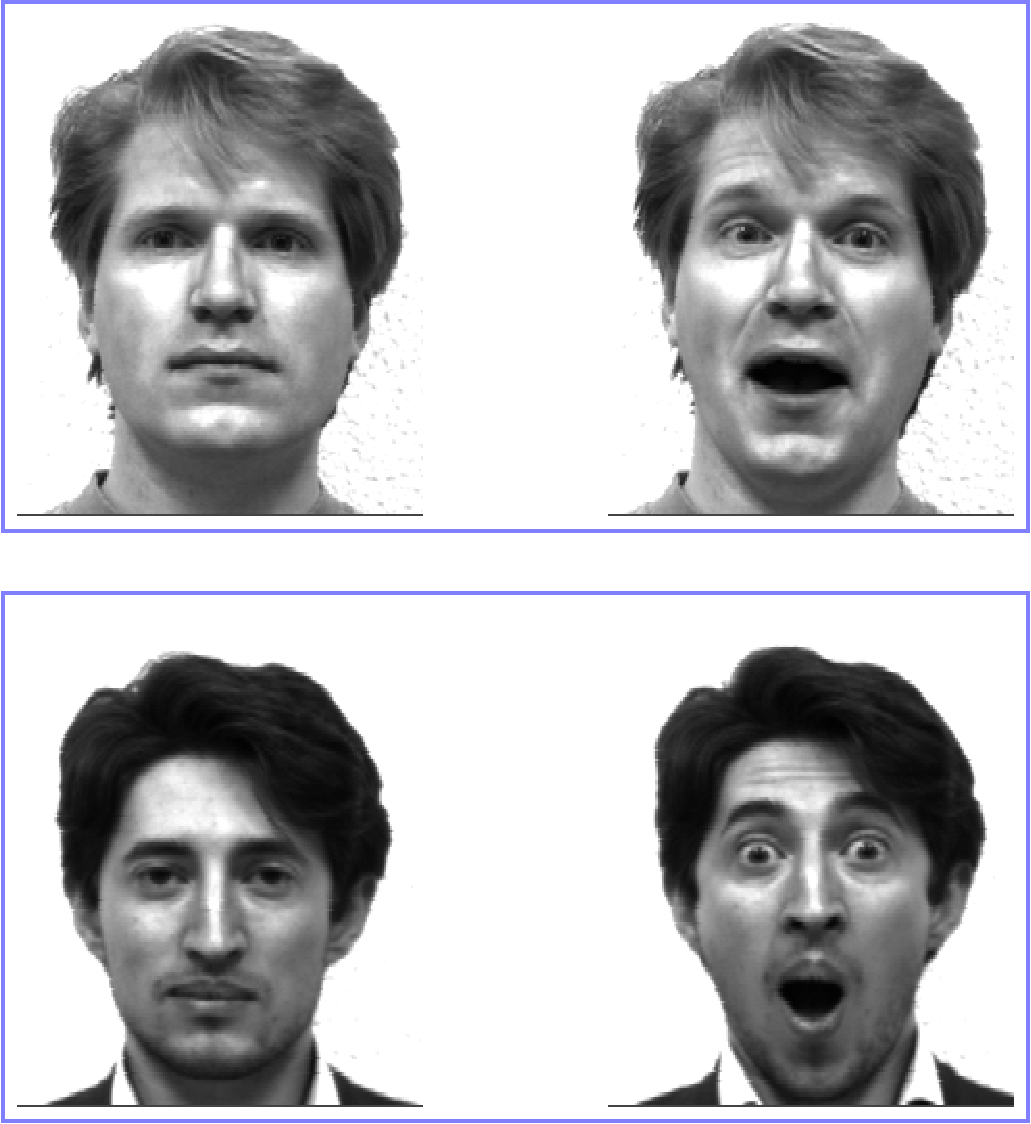
\includegraphics[width=0.4\textwidth]{images/face-recog}}
			    \hspace{0.07\textwidth}
			 \subfigure[Expression recogntion]{\label{fig:expression-recog}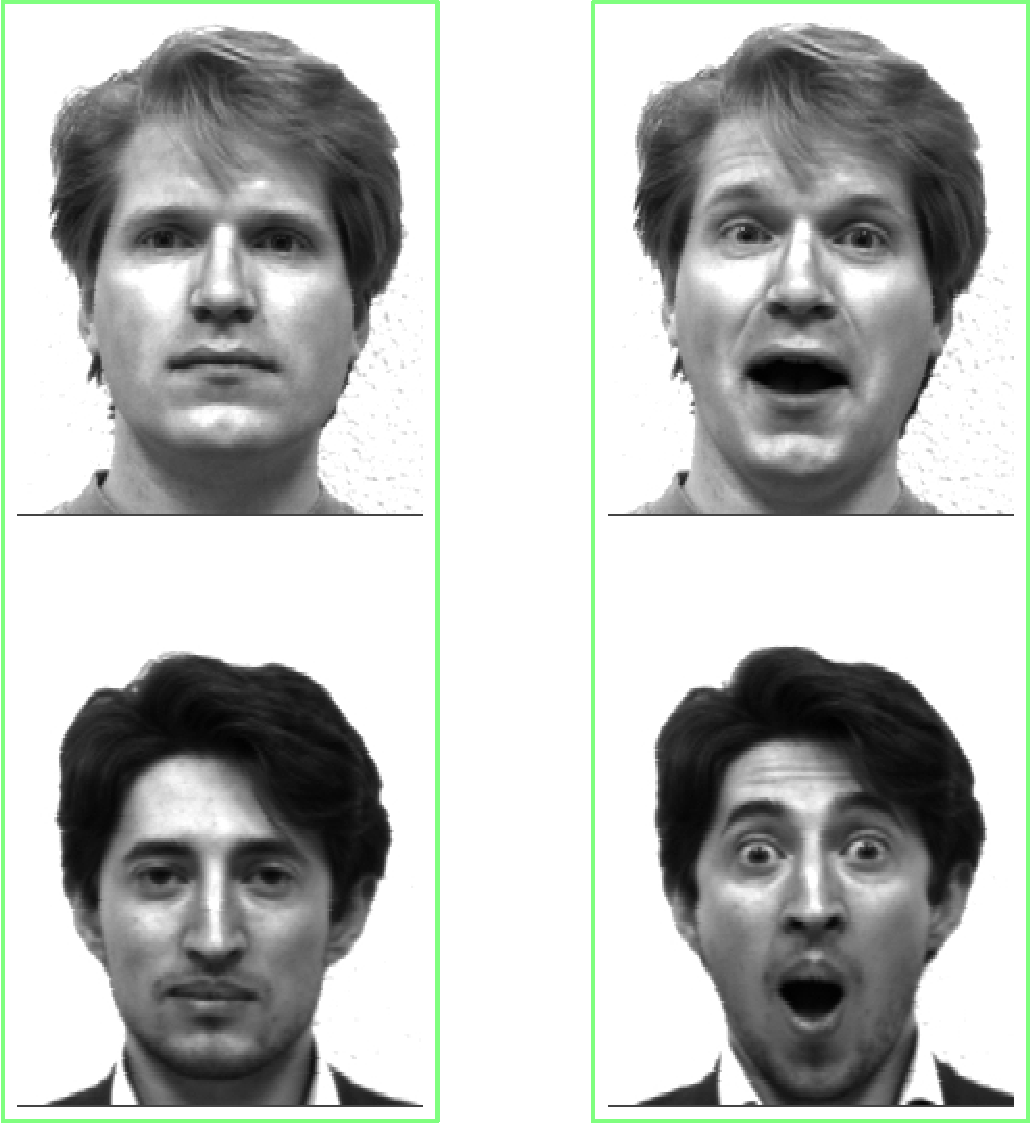
\includegraphics[width=0.4\textwidth]{images/expression-recog}}
		\caption[Motivating the need for a distance metric --- different tasks are solved by different metrics]{On a given data set we might need to perform multiple tasks; in this example: face recognition and expression recognition. The Euclidean metric is not optimal since we want different pairs of equivalence for the two tasks. A good distance metric should be task dependent. These images are an extract from Yale face database.}
		\label{fig:face-recog-vs-expression-recog}
	\end{figure}

The Mahalanobis metric extends the Euclidean distance by incorporating data specific information. But a good metric should be even more flexible than that. Apart from the data set, we are also given a task to perform. We want our metric to extract and discriminate only between information that is relevant to our given task. Take the example of images and face recognition. The pixels from the image background are highly correlated and they reflect the same information: the colour of the background. If the two pictures of the same subject have different backgrounds, we get a high distance between the images. Since we are not interested at all in
the background colour, the metric should identify all the pixels in the background as non-relevant and down-weight their importance. In figure \ref{fig:face-recog-vs-expression-recog}, we illustrate why we need our metric should depend on a given task and why for a given data set it is not optimal to use a fixed metric.

We can further generalize the result from equation \eqref{eq:mahalnobis-distance}.
Instead of setting $\SB$ as the covariance of the data, we let $\SB$ be a different matrix. The problem of determining a suitable matrix
$\SB^{-1}$ is called Mahalanobis (or quadratic) distance metric learning. We note that $\SB^{-1}$ ought to be positive semi-definite $\mathbf{x}\tr\SB^{-1}\mathbf{x} \geq 0, \forall\;\mathbf{x}$. This ensures that the norm is a real value: $d(\mathbf{x},\mathbf{0})\equiv\lVert \mathbf{x}\lVert = \sqrt{\mathbf{x}\tr\SB^{-1}\mathbf{x}}\in\mathbb{R}$.

%We need to further extend the previous result. Given a data set we usually do not care for the data set variance, but want to adapt the weights on the dimensions such that they suit our task. When we want to discriminate among face, we have some dimensions that 

%Equation \eqref{eq:mahalnobis-distance} is the standard definition of the Mahalanobis distance. Since we do not care for any variance in the data, but just for that is representative for our particular task (as discussed in Section \ref{sec:introduction}), we will consider different matrices $S$ that are suitable for the given query. Since we want our metric to discriminate among faces, we down-weight the less informative dimensions. 

\begin{figure}
		 \centering
			  \subfigure[Mahalanobis metric in the original space]{\label{fig:mahalanobis}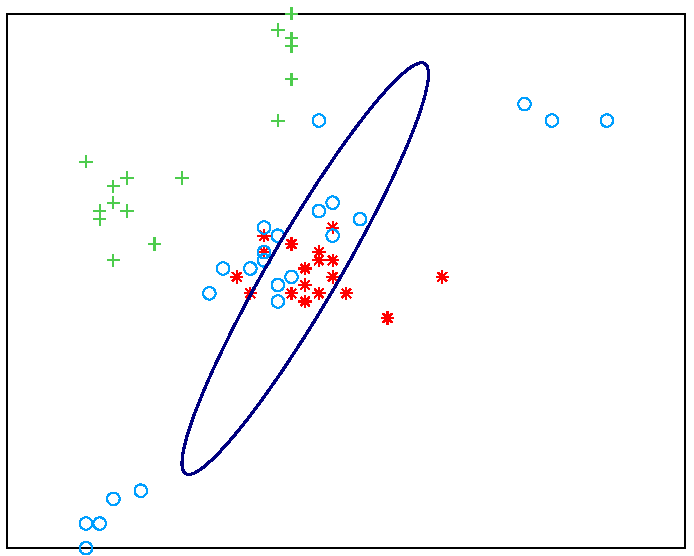
\includegraphics[width=0.45\textwidth]{images/mahalanobis}}
			    \hspace{0.02\textwidth}
			 \subfigure[Euclidean metric in the projected space]{\label{fig:euclidean}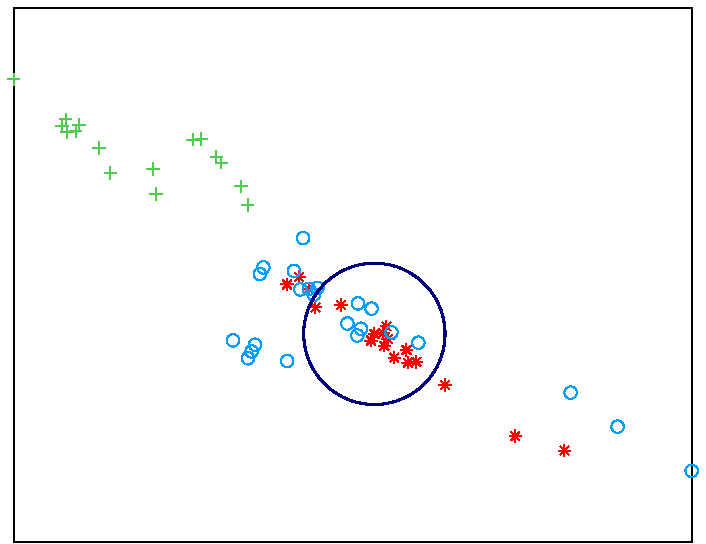
\includegraphics[width=0.45\textwidth]{images/euclidean}}
		\caption[Equivalence between the Mahalanobis metric and its associated linear projection]{Illustration of the equivalence between a Mahalanobis metric in the original data space and an Euclidean metric in the transformed data space. The metrics are denoted by an ellipse and, respectively, a circle whose contours indicate equal distance from the centre point to the rest of the points.}
		\label{fig:mahalanobis-euclidean}
	\end{figure}

There is an interesting equivalence between a Mahalanobis-like metric and a linear transformation. Using the Cholesky decomposition or other matrix square root we can write $\SB^{-1}=\AB\tr\AB$, which gives $\lVert \mathbf{x} \lVert = \sqrt{(\AB\mathbf{x})\tr(\AB\mathbf{x})}$, where $\AB$ represents a linear transformation of the data. Hence, the problem of finding a suitable distance metric $\SB$ is equivalent to the problem of finding a good linear transformation $\AB$ and then applying Euclidean distance in the projected space (figure \ref{fig:mahalanobis-euclidean}). We will discuss these two variants interchangeably and we will often parametrize our models in terms of $\AB$.

\section{Related methods}
\label{sec:related-methods}

The first attempts in metric learning were simple alterations of the Euclidean metric to improve $k$NN performance. For example, \citet{mitchell1997} suggests weighting each attribute of the data points such that the cross validation error is minimized. This technique is equivalent to stretching the axis of the relevant attributes and compressing the axis of the attributes that are less informative. The approach is a special case of learning a diagonal metric, equation \eqref{eq:new-distance}. Another method \citep{moore1994} is to eliminate the least relevant attributes: they are given a weight of zero. Albeit useful, these techniques are restrictive as the feature scaling does not reflect how the data covary.

\citet{hastie1996} proposed discriminant adaptive nearest neighbours (DANN), a method that constructs a local metric for each particular query. The metric is chosen such that it provides the best discrimination amongst classes in the neighbourhood of the query point. This increases the already costly testing time of $k$NN. However, DANN method provides a non-linear metric if we take into account all the possible resulting local linear distance metrics. Even though non-linear transformations are an interesting domain, we will concentrate our attention on linear metrics as they are less prone to over-fitting and easier to learn and represent.

\citet{xing2003} proposed learning a Mahalanobis-like distance metric for clustering in a semi-supervised context. There are specified pairs of similar data points and the algorithm finds the linear projection that minimizes the distance between these pairs without collapsing the whole data set to a single point. This approach is formulated as a convex optimization problem with constraints. The solution is attained using an iterative procedure, such as Newton-Raphson. This method assumes that the underlying density of the data is unimodal which leverages the assumption-free $k$NN. Another drawback is the training time, because the iterative process is costly for large data sets.

Relevant component analysis (RCA; \citealp{bar2003, shental2002}) is another method that makes use of the labels of the classes in a semi-supervised way to provide a distance metric. More precisely, RCA the so-called chunklet information. A chunklet contains points from the same class, but the class label is not known; data points that belong to the same chunklet have the same label, while data points from different chunklets do not necessarily belong to different classes. The main idea behind RCA is to find a linear transformation which ``whitens'' the data with respect to the averaged within-chunklet covariance matrix \citep{weinberger2009}. Compared to the method of \citet{xing2003}, RCA has the advantage of presenting a closed form solution, but it has even stricter assumptions about the data: it assumes that the data points in each class are normally distributed so they can be described using only second order statistics \citep{goldberger2004}.

Large margin nearest neighbour (LMNN; \citealp{weinberger2009}) is a metric learning method that was designed especially for $k$NN classification. LMNN has some similar characteristics to the support vector machine (SVM) technique. As SVM, LMNN brings together points from the same class trying to separate the classes by a certain margin. Also LMNN inherits the convexity property and can be optimize as a semi-definite programming. \citet{weinberger2008} worked on fast metric learning by introducing ball trees to speed up the computations. In \citep{weinberger2008}, they extended LMNN to learn local metrics further improving its performance.

Metric learning is an ongoing research area in machine learning with an abundance of different techniques. For a good report that covers many related methods, the reader is referred to \citep{yang2006}.

\chapter{Neighbourhood component analysis}
\label{ch:nca}

	Neighbourhood Component Analysis (NCA; \citealp{goldberger2004}) learns a Mahalanobis metric that improves the performance of $k$ nearest neighbours ($k$NN). From a practical point of view, NCA  is regarded as a desirable additional step before doing classification with $k$NN. It improves the classification accuracy and it is also provides good low-dimensional representation of the data.

\section{General presentation}
\label{sec:general-presentation}

	Because the goal is to enhance the $k$NN performance, the first idea \citet{goldberger2004}
	had was to maximize the leave one out cross validation performance with respect to a linear projection $\AB$. The procedure can be described as follows: apply the linear transformation $\AB$ to the whole data set, then take each 
	point $\AB\xB_i$ and classify it using $k$NN on the transformed data set $\{\AB\xB_j\}_{j=1}^N$. The matrix $\AB$ that achieves the highest number of correct classifications will be used for testing. Unfortunately, any objective function based on the $k$ nearest neighbours
	is piecewise constant and discontinuous and, hence, hard to optimize. The reason is that there does
	not exist an exact correlation between $\AB$ and the neighbours
	of a given point: a small perturbation in $\AB$ might cause strong changes or, conversely, 
	it might leave the neighbours unchanged.
	
	The authors' solution lies in the concept of \textit{stochastic} nearest
	neighbours. Remember that in the classical scenario, a query point gets the label of the closest point. In the stochastic nearest neighbour 
	case, the query point inherits the label of a neighbour with a probability that is inverse proportional with the distance. The stochastic function is reminiscent of the softmax activation used for neural networks or the generalized logistic function. So $p_{ij}$ is the probability that the point $\xB_j$ is selected as the nearest neighbour of the point $\xB_i$ and it is given by:
	\begin{align}
		p_{ij} = \frac{
						\exp(-d_{ij}^2)
					  }{
						\sum_{\substack{k=1 \\k\neq i}}^N\exp(-d_{ik}^2)
					  },
	\label{eq:stochastic-neighbour}
	\end{align} where $d_{ij} = d(\AB\xB_i;\AB\xB_j) = (\xB_i-\xB_j)\tr\AB\tr\AB(\xB_i-\xB_j)$; also we set $p_{ii}=0$: point~$\xB_i$ cannot pick itself as the nearest neighbour.
	Now we can construct a continuous objective function using the stochastic assignments~$p_{ij}$ which are differentiable with respect to~$\AB$.
	
	A suitable quantity to maximize is the probability of each point of getting correctly classified. A point $\xB_i$ is correctly classified when it is selected by a point $\xB_j$ that has the same label as $\xB_i$:
	\begin{align}
		p_i = \sum_{j\in c_i} p_{ij}.
	\end{align}
	
	The objective function considers each point in the data set and incorporates their probability of belonging to the true class:
	\begin{align}
		f(\AB) &= \sum_{i=1}^N p_i\notag\\
			   &= \sum_{i=1}^N \sum_{j\in c_i} \frac{
								\exp(-d_{ij}^2)
							  }{
								\sum_{k\neq i}\exp(-d_{ik}^2)
							  }.
	\label{eq:nca-obj}
	\end{align}
	The score given by the objective function can be interpreted as the expected number of the correctly classified points.
	
	We maximise $f(\AB)$ using an iterative gradient based solver such as gradient ascent, conjugate gradients or delta-bar-delta, see Subsection \ref{subsec:optimization}. For the optimisation, we need the numerical expression of the gradient. If we differentiate with respect to $\AB$, we obtain:
	\begin{align}
	  \frac{\partial f}{\partial
	\AB}=2\AB\sum_{i=1}^{N}\left(p_i\sum_{k=1}^Np_{ik}\xB_{ik}\xB_{ik}^{\textrm{T}} -
	\sum_{j\in c_i}p_{ij}\xB_{ij}\xB_{ij}^{\textrm{T}} \right)\label{eq:nca-grad},
	\end{align}
	where $\xB_{ij} = \xB_i - \xB_j$. The interested reader can find the derivation of the gradient in the appendix. 
	
	It is useful to note that NCA's objective function is not convex. So care must be taken to avoid poor local optima. The choice of initialization and of the optimization method affect the quality of the final solution. Section \ref{sec:practical-notes} discusses these and other practical issues. On the other hand, the non-convexity property has its advantage. It allows NCA to get good results on more complicated data sets that are not non convex. 

	Another important aspect is the computational cost of the method. For each point, we need to compute all the pairwise distances $d_{ij}$ which has the cost of $\mathcal{O}(dN^2)$. But prior to that, we have to compute the point projections $\{\AB\xB_i\}_{i=1}^N$; this operation is done in $\mathcal{O}(dDN)$ flops. So the total cost of evaluating the objective function $f(\AB)$ is  $\mathcal{O}(dDN+dN^2)$. The cost of the gradient given in the original paper, equation \ref{eq:nca-grad}, scales in $D^2N^2$. We can improve this by ``pushing'' the matrix $\AB$ into the sum:

	This has a cost in $\mathcal{O}(dDN^2)$. However, automatic differentiation (AD) lets us calculate the gradient in the same time as the original objective function \citep{rall1981}. AD uses the chain rule to derivative the objective function; the gradient will consist of elementary functions. Instead of evaluating the complicated analytical gradient, we work on a series of cheap operations. This method is very useful in practice and there exist packages for it in most programming languages. In our implementation we used the analytical differentiation, because we were not aware of AD.

	Chapter \ref{ch:reducing} treats NCA's computational drawback; there are presented different ideas of speeding up the computations.
	
	The general scenario in which NCA is applied can be described by the training and testing steps:
	describe algorithm.
	%\begin{itemize}
	%   \item
	%\end{itemize}
	
\section{Class-conditional kernel density estimation interpretation}
\label{sec:cc-kde}
	
	\begin{figure}
	  \centering
	  \subfigure[Illustration of the class as a mixture of
	Gaussians.]{\label{fig:mog}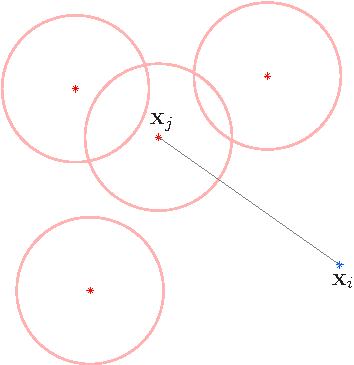
\includegraphics[width=6cm]{images/mog}}
	%\subfigure[The projection $\AB$ applied to the whole data set
	%$\mathcal{D}$.]{\label{fig:sub-sampling-2}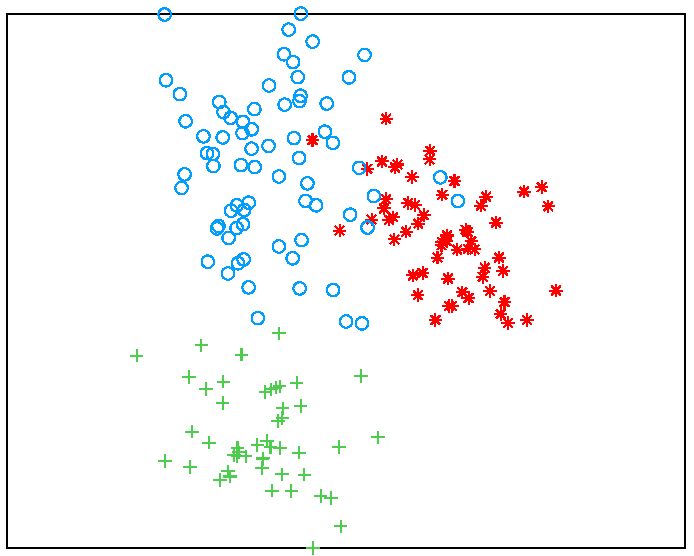
\includegraphics[width=0.48\textwidth]{images/sub-sample-2}}
	  \caption{Formulating NCA as a class-conditional kernel density estimation
	framework.}
	  \label{fig:kde}
	\end{figure}
	
	In this section we will present NCA into a class-conditional kernel density
	estimation framework. This interpretation will allow us to understand what are
	the assumptions behind NCA. Moreover, this also offers the possibility of
	altering the model in a suitable way that is efficient for computations. We will
	see this in the sections \ref{sec:approximate} and \ref{sec:exact-computations}.
	Similar ideas were previously presented by and , but the following were derived
	independently and they offer different insights. The following interpretation
	was inspired by the probabilistic $k$NN presented by \citet{barber2011}.
	
	We start with the basic assumption that each class can be modelled by a mixture
	of Gaussians. For each of the $N_c$ data points in class $c$ we consider a
	Gaussian ``bump'' centred around it. From a generative perspective, we can view
	that each point $\xB_j$ can generate a point $\xB_i$ with a probability given by
	an isotropic normal distribution with variance $\sigma^2$:
	\begin{align}
	    p(\xB_i|\xB_j) &= \mathcal{N}(\xB_i|\xB_j, \sigma^2\mathrm{I}_D) \\
	                   &= \frac{1}{(2\pi)^{D/2}}\exp \left\{-\frac{1}{2\sigma^2}
	(\xB_i - \xB_j)^\mathrm{T}(\xB_i - \xB_j)\right\}.
	\end{align}
	
	By changing the position of the points through a linear transformation $\AB$,
	the probability changes as follows:
	\begin{align}
	    p(\AB\xB_i|\AB\xB_j) \propto \exp \left\{-\frac{1}{2\sigma^2} (\xB_i -
	\xB_j)^\mathrm{T}\AB^\mathrm{T}\AB(\xB_i - \xB_j)\right\}.
	\end{align}
	
	We can note that this is similar to the $p_{ij}$ from NCA. Both
	$p(\AB\xB_i|\AB\xB_j)$ and $p_{ij}$ are directly proportional with the same
	quantity.
	
	Using the mixture of Gaussians assumption, we have that the probability of a
	point of being generated by class $c$ is equal to the sum of all Gaussians in
	class $c$:
	\begin{align}
	    p(\xB_i|c) &= \frac{1}{N_c}\sum_{\xB_j \in c} p(\xB_i|\xB_j)\\
	               &= \frac{1}{N_c}\sum_{\xB_j \in c} \mathcal{N}(\xB_i|\xB_j,
	\mathrm{I}_D).
	\end{align}
	
	However, we are interested on the inverse probability, given a point $\xB_i$
	what is the probability of $\xB_i$ belonging to class $c$. We can obtain an
	expression for $p(c|\xB_i)$ using Bayes' theorem:
	\begin{align}
	    p(c|\xB_i) = \frac{p(\xB_i|c)p(c)}{p(c|\xB_i)} =
	\frac{p(\xB_i|c)p(c)}{\sum_{c} p(\xB_i|c)p(c)}.
	    \label{eq:nca-cc-kde-bayes}
	\end{align}
	
	Now if further consider the classes to be equal probable (which might a
	reasonable assumption if we have no a priori information) we arrive at result
	that resembles the expression of $p_i$ (see equation):
	\begin{align}
	%   &p(c|\xB_i) = \frac{p(\xB_i|c)}{\sum_{c} p(\xB_i|c)}\\
	    p(c|\AB\xB_i) = \frac{
	                \frac{1}{N_c}\sum_{\xB_j \in
	c}\exp\left\{-\frac{1}{2\sigma^2}(\xB_i -
	\xB_j)^\mathrm{T}\AB^\mathrm{T}\AB(\xB_i - \xB_j)\right\}
	                }
	                {
	                \frac{1}{N_{c'}}\sum_{c'} \sum_{\xB_k \in
	c'}\exp\left\{-\frac{1}{2\sigma^2}(\xB_i -
	\xB_k)^\mathrm{T}\AB^\mathrm{T}\AB(\xB_i - \xB_k)\right\}
	                }
	\end{align}
	
	%In the numerator we have the sum of
	We are interested in predicting the correct class of the point $\xB_i$. So we
	try to find that linear transformation $\AB$ that maximises the class
	conditional probability of this point $p(c_i|\xB_i)$ to its true class $c_i$.
	\begin{align}
	    f(\AB) = \sum_i p(c_i|\AB\xB_i).
	    \label{eq:nca-cc-kde-obj}
	\end{align}.
	
	The gradient of the objective function is the following:
	\begin{align}
	    \frac{\partial f}{\partial \AB} =
	      \sum_i \left\{
	                \frac
	                {
	                    \frac{\partial p(\AB\xB_i|c)}{\partial \AB}p(c)
	                }
	                {
	                    \sum_c p(\xB_i|c)p(c)
	                }
	                - \underbrace{\frac{
	                    p(\AB\xB_i|c)p(c)
	                }{
	                    \sum_c p(\AB\xB_i|c)p(c)
	                }}_{p(c|\AB\xB_i)}
	                \frac{
	                    \sum_c \frac{\partial p(\AB\xB_i|c)}{\partial \AB}p(c)
	                }{
	                    \sum_c p(\AB\xB_i|c)p(c)
	                }
	             \right \}.
	    \label{eq:nca-cc-kde-grad}
	\end{align}
	

\section{Practical notes}
\label{sec:practical-notes}

	This section provides some practical advice for the questions 
	that can be raised while implementing NCA. 
	While NCA is not that hard to implement, there is needed certain care
	in order to achieve good solutions.

\subsection{Optimization methods}
\label{subsec:optimization}

	The function $f(\AB)$, equation \ref{eq:nca-obj}, can be maximised using any gradient based optimizer. We considered two popular approaches for our implementation: gradient ascent and conjugate gradients. These are only briefly presented here. The interested reader is pointed to \citet{bishop1995}.

	\subsubsection*{Gradient ascent}

	Gradient ascent is one of the simplest optimisation methods. It is an iterative algorithm that aims to find the maximum of a function by following the gradient direction at each step. The entire procedure is summarized by algorithm \ref{alg:gd}.
      
	\begin{algorithm} 
		\caption{Gradient ascent (batch version)} 
		\label{alg:gd}  
		\begin{algorithmic}[1]                    % enter the algorithmic environment
			\REQUIRE Data set $\mathcal{D}=\{\xB_1,\cdots,\xB_N\}$.
			\STATE{ Get initial $\AB_0$ } \label{alg:gd-init}
			\REPEAT
				\STATE {Update parameter: $\AB_{t+1}\leftarrow \AB_{t} + \eta\frac{\partial
f(\AB_{t},\mathcal{D})}{\partial\AB}$}
				\STATE {Update learning rate $\eta$}
				\STATE {$t\leftarrow t+1$}
			\UNTIL {convergence}
			\RETURN $\AB_{t}$.
		\end{algorithmic}
	\end{algorithm}

	There are three aspects we need to carefully consider:
	\begin{enumerate}
	 \item The algorithm starts the search in the parameter space from the an initial parameter~$\AB_0$. Different values for $\AB_0$ will give different final solutions. In the NCA context, initialization is related to finding a good initial linear transformation; this is discussed  separately in subsection \ref{subsec:initialization}. For the moment, we can assume the values of $\AB_0$ are randomly chosen.
	 \item The parameter $\eta$ is called \textit{step size} or, in neural networks related literature, it also known as \textit{learning rate}. As name suggests, $\eta$ controls how much we move the parameter in the gradient direction. 

	The learning rate can be either fixed or adaptive. For the first case, choosing the correct value for $\eta$ is critical. If $\eta$ is set too large, the algorithm diverges. On the other hand, a small $\eta$ results in slow convergence. 

	Usually, a variable learning rate $\eta$ is preferred since it is more flexible. The ``bold driver'' is a heuristic for automatically modifying $\eta$ during training. The idea is to gradually increase the learning rate after each iteration as long as the objective function keeps improving. Then we go back to the previous position and start decreasing the learning rate until a new increase in the function is found. This procedure is described in algorithm. The parameters indicate how much the learning rate is adjusted at each step. Usually, $\rho=1.1$ and $\sigma=0.5$.
	
	Another way is to change the learning rate~$\eta$ using a decreasing rule proportional to the number of current iteration: $\eta=\frac{\eta_0}{t+t_0}$. Now we have two parameters instead of one. Intuitively, $\eta_0$ can be regarded as the initial learning rate and $t_0$ is the number of iterations after which $\eta_0$ starts to drop off. Using a learning rate of such form is especially motivated in the stochastic gradient case. If $\eta\propto 1/t$, the algorithm converges to the true minimum as $t$ goes to infinity. However, in practice the converges is very slow; so setting the constant $\eta_0$ and~$t_0$ is important for reaching a good solution in a short time. Leon Bottou recommends to set $\eta_0$ to be regularization value and select $t_0$ such that the update will result in a sensible new value for $\AB$. Since we did not use regularization, we followed some of the tricks presented in \citep{lecun1998}. We fixed the value for $\eta_0$ and we did an exponential search for $t_0$ using a cross validation set.

% 	A popular choice for an 
	 \item Convergence. We set a maximum number of iterations. Also we use ``early stopping'': we monitor the performance of the new $\AB$ on a cross validation set. If the objective function did not increase for more than a preset number of iterations we stop and return to the previous best solution. This avoids overfitting.
	\end{enumerate}


% 	The notation $\frac{\partial f(\AB_t,\mathcal{D})}{\partial \AB}$

	\subsubsection*{Conjugate gradients}
	

% \begin{itemize}
%     \item We have the first-order gradient information; so, we
%         can use any gradient based method.
%     \item Gradient descent is an iterative algorithm that uses
%         first-order information to find a minimum of a
%         function. At each step, it proposes to go in the
%         steepest direction, \ie, the direction with largest
%         gradient. It is a very simple to implement method, but
%         suffers from known convergence drawbacks. For example,
%         there might appear the zig-zagging effect it depends
%         on some critical parameters which make it difficult to
%         use in practice. These are the learning rate $\eta$
%         and the convergence conditions.
%     \item Common choices for $\eta$ are either using a
%         constant step or decrease it gradually. Using a
%         constant step size can make the algorithm diverge.
%     \item There are different other heuristics that make this
%         more efficient. One of these is the bold-driver trick.
%     \item A learning rate decreasing procedure is to set
%         $\eta=\frac{\eta_0}{t + t_0}$, where $t$ represents
%         the iteration number, $\eta_0$ and $t_0$ are
%         constants. So, we end up with two hyper-parameters
%         instead of one. There are various trick of tuning
%         them. Leon Bottou mentions that a common value for
%         $\eta_0$ is to be equal to the regularization variable
%         and $t_0$ should then be selected such that the
%         updates . In our implementation, because we did not
%         use a regularization term, we set $\eta_0$ to a fix
%         value and then we did an exponential search for $t_0$.
%     \item One might also try to use momentum. For further
%         useful advice on optimization one should consult
%         BackProp.
%     \item An improved version of the gradient descent is the
%         conjugate gradients algorithm. This has better
%         convergence.
% \end{itemize}

\subsection{Initialization}
\label{subsec:initialization}

    \begin{figure}
	  \centering
	  \subfigure[Initial random projection]{\label{fig:init-1}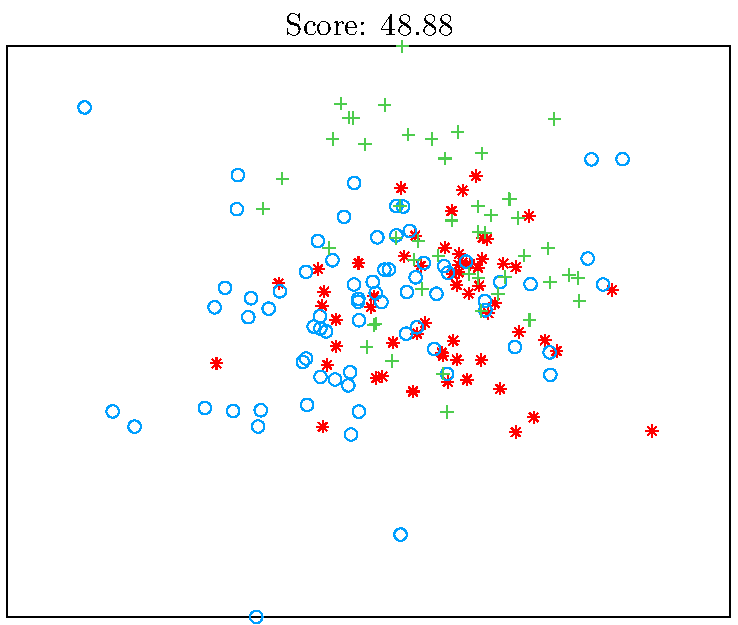
\includegraphics[width=0.49\textwidth]{images/wine-init-1}}
	  \subfigure[NCA projection after random initialization]{\label{fig:init-2}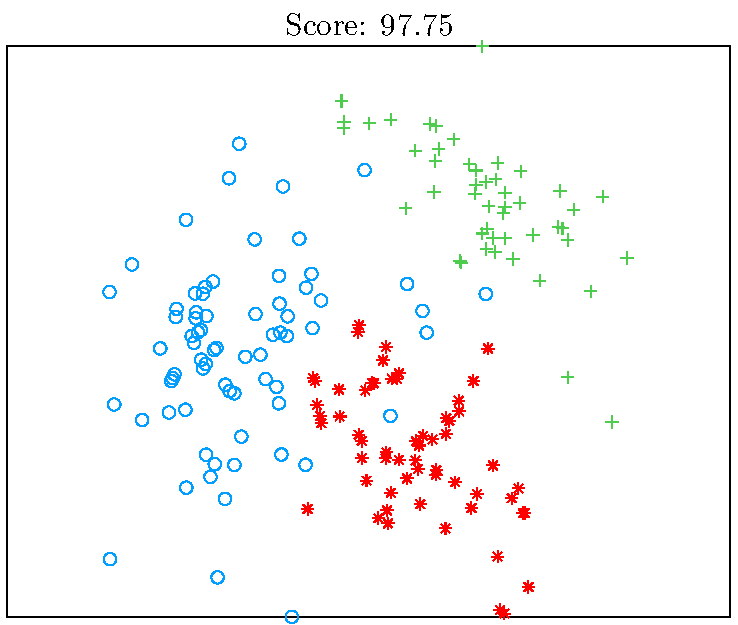
\includegraphics[width=0.49\textwidth]{images/wine-init-2}}

	  
	  \subfigure[Initial projection using PCA]{\label{fig:init-3}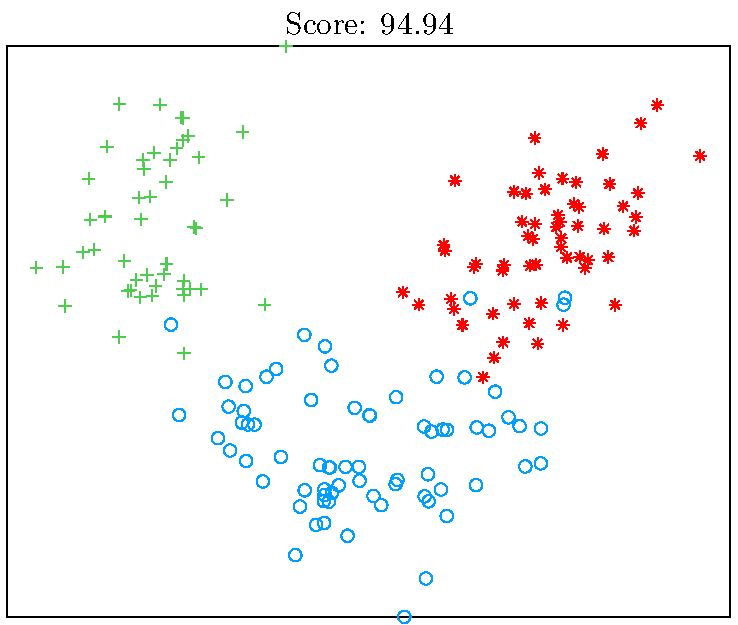
\includegraphics[width=0.49\textwidth]{images/wine-init-3}}
	  \subfigure[NCA projection after PCA initialization]{\label{fig:init-4}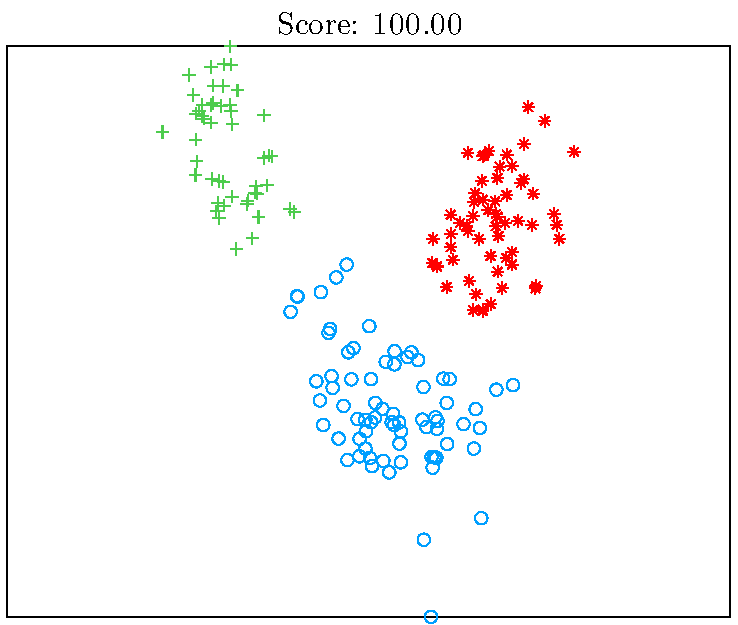
\includegraphics[width=0.49\textwidth]{images/wine-init-4}}

	  
	  \subfigure[Initial projection using LDA]{\label{fig:init-7}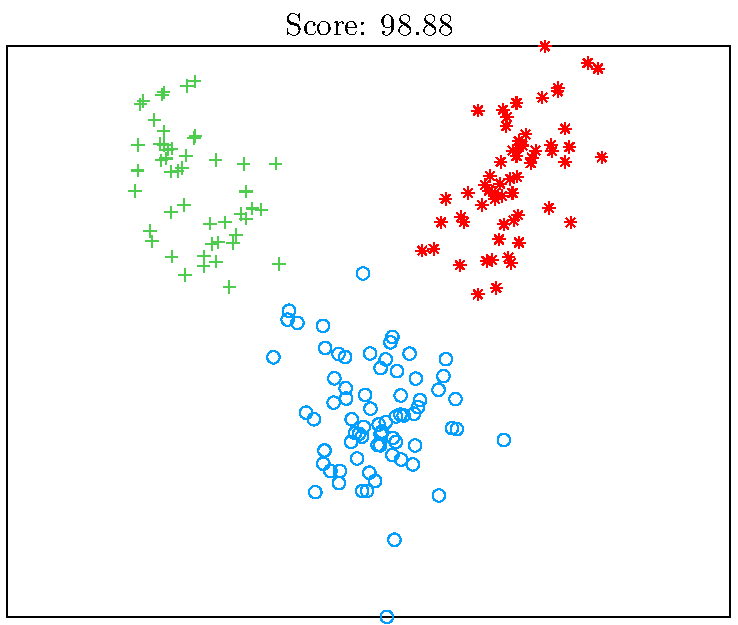
\includegraphics[width=0.49\textwidth]{images/wine-init-5}}
	  \subfigure[NCA projection after LDA initialization]{\label{fig:init-8}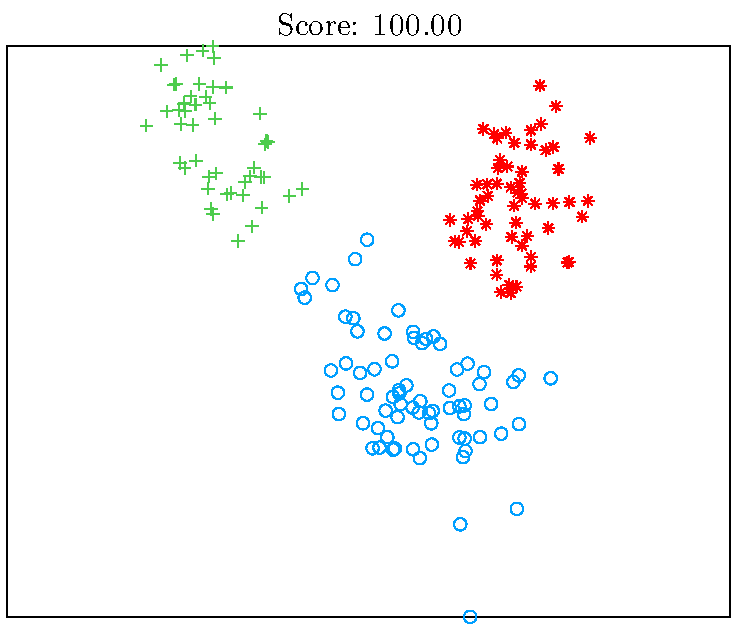
\includegraphics[width=0.49\textwidth]{images/wine-init-6}}
	  
	  \caption{\small Results for different initializations (random, PCA and LDA) on \texttt{wine} data set. The images on the left side represent the projections of the data set using the initial $\AB$. The images on the right side are data set projection with the final $\AB$. Above each figure there is presented the LOOCV score which is normalized to 100.}
	  \label{fig:init}
    \end{figure}

    Initialization is important because the function $f(\AB)$ is not convex. The quality of the final solution relies on the starting point of the optimisation algorithm. A general rule of thumb is to try multiple initial seeds and select that final $\AB$ that gives the highest score.

    We have already mentioned random initialization in subsection \ref{subsec:optimization}. Beside this, we can linear transformations that are cheap to compute. Such examples include  principal component analysis (PCA; \citealp{pearson1901}), linear discriminant analysis (LDA; \citealp{fisher1936}) and relevant component analysis (RCA; \citealp{bar2003}). For completeness, we give here the equations and also include further notes:
        \begin{itemize}
            \item  PCA finds an orthogonal linear
                transformation of the data. This is
                obtained by computing the
                eigendecomposition of the outer covariance
                matrix:
                \begin{align}
                    \SB = \frac{1}{N}\sum_{i=1}^N (\xB-\muB)(\xB-\muB)\tr.
                    \label{eq:pca-1}
                \end{align}

            \item LDA finds a linear transformation $\AB$ by maximizing the
variance between classes $\SB_B$ relative to the amount of within-class variance
$\SB_W$:
            \begin{align}
             \SB_B &=
\frac{1}{C}\sum_{c=1}^{C}\boldsymbol\mu_c\boldsymbol\mu_c\tr\label{eq:lda-1}\\
             \SB_W &= \frac{1}{N}\sum_{c=1}^{C}\sum_{i \in
c}(\mathbf{x}_i-\boldsymbol{\muB}_c)(\mathbf{x}_i-\boldsymbol{\mu}_c)\tr.\label{eq:lda-2}
            \end{align}

            The projection matrix $\AB$ that achieves this maximization consists
of the eigenvectors of $\SB_W^{-1}\SB_B$.

            Unlike PCA, LDA makes use of the class labels and this
usually guarantees a better initial projection.

            \item RCA finds a linear transformation $\AB$
                that ``whitens'' the data with respect to
                the within-chunklet covariance matrix.
                Because for NCA we restrict ourselves to
                fully labelled data, the within-chunklet
                covariance is the within-class covariance
                $\SB_W$, Equation \ref{eq:lda-2}. The
                whitening transformation is then
                $\AB=\SB_W^{-1/2}$.
        \end{itemize}

        If the projection is full-rank, $\AB\in\mathbb{R}^{D\times D}$, other obvious initializations are the identity matrix $\AB=\mathrm{I}_D$ and the Mahalanobis linear transformation $\AB=\SB^{-1/2}$.

	If we want to learn a low-rank projection, $\AB \in \mathbb{R}^{d\times D},d<D$, then we can still use the eigendecomposition based methods. We construct $\AB$ using only the top $d$ most
        discriminative eigenvectors, \ie, those eigenvectors that have the
        highest eigenvalues associated.

        From our experiments, we conclude that a good
        initialization reflects in a good solution and a better convergence; this benefits are more evident
        large data sets. As advertised in , we found RCA to work the best. Figure depicts initialization effects on a small data set.

\subsection{Numerical issues}
\label{subsec:numerical-issues}

	Numerical problems can easily appear when computing the soft assignments $p_i$. If a point
        $\xB_i$ is far away from the rest of the points, the stochastic probabilities $p_{ij}, \forall j,$ are all 0 in numerical precision. Consequently, the result $p_i$ is undetermined: $\frac{0}{0}$. 
	To make an idea of how far $\xB_i$ has to be for this to happen, let us consider an example in \textsc{Matlab}. The answer to 
        \texttt{exp(-d\^{}2)} is \texttt{0} whenever \texttt{d} exceeds \texttt{30} units.
	This is problematic in practice, since distances larger than 30 often appear. Some common cases include data sets that contain outliers or data sets that present a large scale. 

	The large scale effect can be partially alleviated if we initialize $\AB$ with small values. This is idea was used by Laurens van der Maaten in his implementation: \texttt{A = 0.01*randn(d,D)}. However, this does not guarantee to compensate the scale variation for any data set.

% 	projection $\AB$ does not compensate for the scale

	A more robust solution is to normalize the
        data, \ie, centre and making it unit variance:
        \begin{align}
            x_{ij} \leftarrow \frac{x_{ij} - \mu_j}{\sigma_j}, i =
	    \{1,\cdots,N\}, j = \{1,\cdots,D\}.
        \end{align}
        In this case, we have to store the initial mean and variance of the data
        and, at test time, transform the test data accordingly: subtract the mean and scale it using the variance coefficients. The variance scaling can be regarded as a linear transformation. We can combine this transformation with the learnt transformation $\AB$ and get:
        \begin{align}
            \AB_{\text{total}} \leftarrow \AB  \cdot \begin{pmatrix}
                  \sigma_1 &  \cdots & 0 \\
                  \vdots  &   \ddots & \vdots  \\
                  0 & \cdots & \sigma_D
                 \end{pmatrix}.
        \end{align}

	
	In general, data normalization avoids numerical issues for the first iterations. But during training, the scale of $\AB$ increases and data points can be ``thrown'' away. We adopt a rather simplistic approach to avoid any numerical problems: replace $p_i$ with a very small value whenever we are in the $\frac{0}{0}$ case, as in Laurens van der Maaten implementation. In \textsc{Matlab}, this is done using the following command \texttt{max(p\_i,eps)}. 
    
	A more robust more rigorous way of dealing with this by multiplying both the numerator and denominator of $p_i$ with a certain quantity $\exp(L)$:
	\begin{align}
	  p_i = \frac{\sum_{j\in c_i} \exp(L-d_{ij}^2)}{\sum_{k\neq i} \exp(L-d_{ik}^2)},
	\end{align}
	where $L = \min_{k\neq i} d_{ik}^2$. This value of $L$ ensures that at least one term in the denominator does not undeflow.

	In our implementation, we preferred the previous trick because of its simplicity and speed.

\subsection{Regularization}
\label{subsec:regularization}

  Although the original paper \citep{goldberger2004} claimed that there were no problems with overfitting, we observed that NCA objective function has the tendency to increase the scale of the linear projection~$\AB$. \citet{butman2008} pointed out that this is especially problematic for data sets whose size~$N$ is significantly smaller than the dimensionality~$D$. In such a case, the linear transformation~$\AB$ can be chosen to project each point~$\xB_i$ to a pre-specified a location~$\yB_i$. The values of $\AB$ are obtained by solving the linear system:
  \begin{align}
    \AB\xB_i = \yB_i, \quad i = \{1,\cdots,N\}.
  \end{align}

  Because the system has more equations $dN$ than unknowns $dD$, it has exact solutions. If we set the same positions $\yB_i$ for points in the same class, we can virtually increase the scale of the projection to infinity and get an error-free classification. This degeneracy can be corrected with the help of regularization. We alter the objective function by subtracting a regularization term proportional with the magnitude of $\AB$. This gives:
  \begin{align}
    g(\AB) = f(\AB) - \lambda \sum_{i=1}^d\sum_{j=1}^D A_{ij}^2.\\
            \frac{\partial g}{\partial \AB} = \frac{\partial f}{\partial \AB} - 2\lambda\AB,
  \end{align}
  where $\lambda$ is a positive constant that is tuned via cross-validation.

  Another effect of a large scale linear projection $\AB$ is the fact that only the nearest neighbour is considered for each point. This is not usually the optimal thing to do, so regularization is also used to prevent this \citep{singh2010}.

  In our implementation, we use ``early stopping'' technique which has a similar effect to regularization. 

% \begin{itemize}
%     \item NCA favours 1NN and large scale linear projections
%         $\AB$. This is not usually the optimal thing.
%     \item We can correct this using regularization, as pointed
%         out in \citep{singh2010}.
%         
%     \item On the other hand, it is not clear how to set the
%         regularization parameter $\lambda$ and how to choose
%         the number of nearest neighbours for classification.
% \end{itemize}

\subsection{Doing classification}
\label{subsec:doing-classification}

  For testing, \citet{goldberger2004} considered only $k$NN decision rule. Since we are optimizing a particular function~$f(\AB)$, another sensible tool for classification is an NCA based function. If we are using the probabilistic interpretation, section \ref{sec:cc-kde}, a query point~$\xB_i$ is labelled with most probable class~$c$:
  \begin{align}
     c = \operatorname{argmax}_cp(c|\xB_i).
  \end{align}

  This can be re-written in NCA specific notation:
  \begin{align}
    c = \operatorname{argmax}_c\frac{\sum_{j\in c}p_{ij}}{\sum_k p_{ik}}.
    \label{eq:nca-cls}
  \end{align}

  In our experiments, $1$NN and the NCA classification rule described by equation \eqref{eq:nca-cls} give very similar results if we train $\AB$ using the un-regularized function~$f(\AB)$. On the cases where we used early stopping, the NCA classification rule yielded better performances, see chapter \ref{ch:evaluation}. In this case, $k$NN with $k>1$ should also perform better than simple $1$NN.

\subsection{Dimensionality annealing}
\label{subsec:dimensionality-annealing}

  Dimensionality annealing is an approach to learning a low-rank metric in an way that avoids local optima (Hinton and Murray, oral communication). We start with a full rank projection $\AB$ and gradually reduce the rank by introducing regularization terms on the lines of $\AB$. Compared with the classical regularization procedure, subsection \ref{subsec:regularization}, here we use a regularization term on each of the dimension $d$. The new objective function and its gradient are given by the following equations:
    \begin{align}
            g(\AB) = f(\AB) - \sum_{i=1}^d\lambda_i\sum_{j=1}^D A_{ij}^2\\
            \frac{\partial g}{\partial \AB} = \frac{\partial f}{\partial \AB} - 2\begin{pmatrix}
                              \lambda_1A_{11} &  \cdots & \lambda_1A_{1D} \\
                              \vdots  &   \ddots & \vdots  \\
                              \lambda_dA_{d1} & \cdots & \lambda_dA_{dD}
                             \end{pmatrix}.
     \end{align}

  A large value of $\lambda_d$ will impose a small magnitude of $\AB$ on dimension $d$. We increase $\lambda_d$ slowly; this permits for the rest of the values of $\AB$ to readjust. We clarify these steps in algorithm \ref{alg:dimensionality-annealing}.

  \begin{algorithm} 
	\caption{Dimensionality annealing} 
	\label{alg:dimensionality-annealing}  
	\begin{algorithmic} [1]                 % enter the algorithmic environment
		\REQUIRE Data set $\mathcal{D}=\{\xB_1,\cdots,\xB_N\}$, initial linear
transformation $\AB\in\mathbb{R}^{D\times D}$ and low dimension~$d$.
		\FOR {$i=1,\cdots,D-d$}
		  \STATE {Select dimension $d$ to anneal} \label{alg:dim-anneal-select-dim}
		  \FOR {$j=1,\dots,P$}
		    \STATE {Increase regularization coefficient $\lambda_d \leftarrow \lambda_d + \Delta\lambda$}
		    \STATE {Optimize function $g$: $\AB = \AB + \eta \frac{\partial g(\AB,\mathcal{D},\lambdaB)}{\partial \AB}$}
		  \ENDFOR
		\ENDFOR
	\end{algorithmic}
\end{algorithm}

  There are several notes to be made. There are alternatives for selecting the dimension $d$ we want to anneal, step \ref{alg;dim-anneal-select-dim} from algorithm \ref{alg:dimensionality-annealing}. We can choose $d$ to be the direction that has:
    \begin{itemize}
     \item minimum variance in our data set $\{\AB\xB_i\}_{i=1}^N$
     \item minimum variance in the projected data set $\{\AB\xB_i\}_{i=1}^N$
     \item smallest magnitude in $\AB$.
    \end{itemize}

    The function optimization step can be done either by gradient ascent or conjugate gradients. It is possible to do conjugate gradients for a small number of iterations, typically 2 or 3.

    After a dimension is annealed, we reach the end of the inner for loop, we can remove that particular dimension; for example set the elements on the $d$ row equal to 0.

    A further idea would be to run conjugate gradients until convergence initialized with low dimensional $\AB$ returned by algorithm \ref{alg:dimensionality-annealing}.

\chapter{Reducing the computational cost}
\label{ch:reducing}

As emphasized in section \ref{sec:general-presentation}, neighbourhood component analysis (NCA) is a computationally expensive method. The evaluation of its objective function is quadratic in the size of the data set. Given that the optimization is done iteratively, NCA becomes prohibitively slow when applied on large data sets. There is only little previous work that uses NCA for large scaled applications. One example is \citet{singh2010}, who parallelizes the computations across multiple computers and adopts various heuristics to prune terms of the objective function and the gradient.

This chapter aims to continue the existing work and to present a series of methods that can improve NCA's speed. Most of these ideas are new in the context of NCA. We start with simple approaches like sub-sampling (section~\ref{sec:sub-sampling}) and mini-batch methods (sections~\ref{sec:mini-batches} and~\ref{sec:stochastic-learning}). For further speed-ups, we proceed with more sophisticated ideas (starting from section~\ref{sec:approximate}). 
%They are also quite versatile. Each method proposes a new objective function and can be regarded as an independent model on its own.

% \begin{itemize}
% 	\item As mentioned in section , evaluating the objective function needs
% computing all the pairwise distances between the points. Also, the evaluating
% the gradient is expensive. This is done in $\mathcal{O}(N^2D^2)$ flops. So it is
% not trivial to successfully use NCA on large data sets.
% 	\item  Most of the methods rely on the fact that
% the learnt metric is low ranked.
% 	\item Every method presented can be regarded as an alteration of the original
% objective function. We basically change our objective function such that the new
% objective will have a reduced cost.
% \end{itemize}

\section{Sub-sampling}
\label{sec:sub-sampling}

Sub-sampling is the simplest idea that can help speeding up the computations.
For the training procedure we use a randomly selected sub-set $\mathcal{D}_n$ of
the original data set $\mathcal{D}$:
 \[
 	\mathcal{D}_n = \{ \xB_{i_1},\cdots,\xB_{i_n} \} \subseteq \mathcal{D}.
 \]
 If $n$ is the size of the sub-set then the cost of the gradient, equation~\eqref{eq:nca-grad-alt}, is reduced to
$\mathcal{O}(dDn^2)$. After the projection matrix $\AB$ is learnt, we apply it to the whole data set $\{\xB_i\}_{i=1}^N$. Then all the new data points $\{\AB\xB_i\}_{i=1}^N$ are used for
classification. The cost of the classification is $\mathcal{O}(dN)$ which is linear in the total number of points $N$.

While easy to implement, this method discards a lot of the information available.
Also it is affected by the fact the sub-sampled data has a thinner density
than the real data. The distances between the randomly selected points are larger than they are in the full data set. This causes the scale of the projection matrix $\AB$ not to be large enough. In figure \ref{fig:sub-sampling} we illustrate that a seemingly perfect linear transformation of the sub-sampled data set does not correspond to a good transformation of the entire data set.

\begin{figure}
  \centering
  \subfigure[Learnt projection $\AB$ on the sub-sampled data set
$\mathcal{D}_n$.]{\label{fig:sub-sampling-1}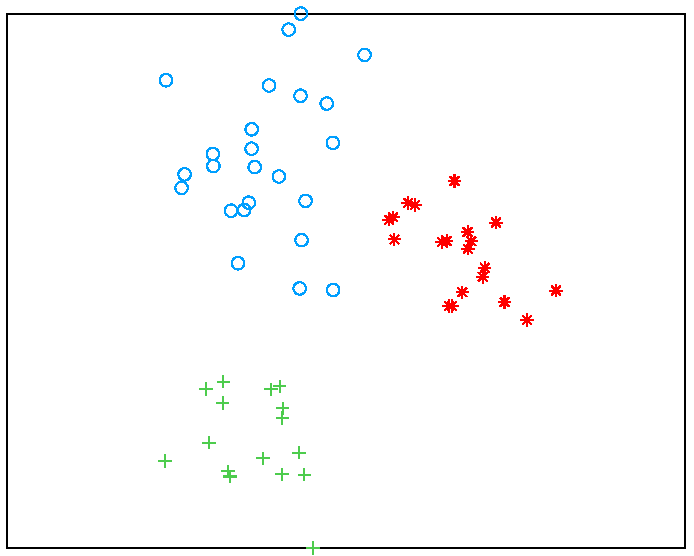
\includegraphics[width=0.48\textwidth]{images/sub-sample-1}}
\subfigure[The projection $\AB$ applied to the whole data set
$\mathcal{D}$.]{\label{fig:sub-sampling-2}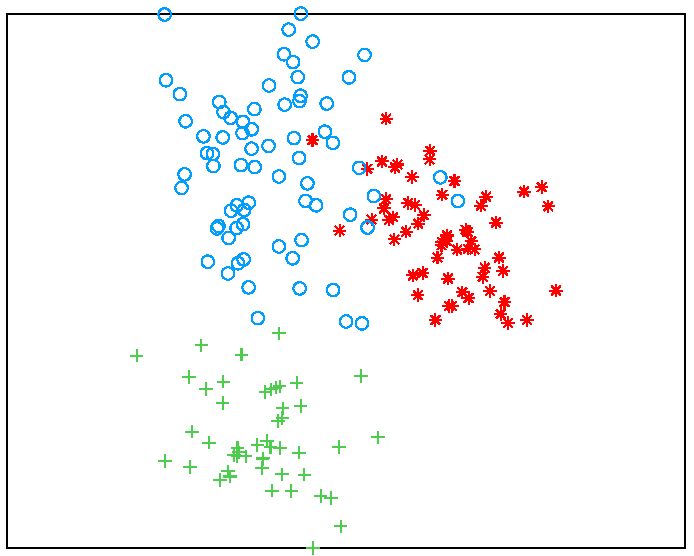
\includegraphics[width=0.48\textwidth]{images/sub-sample-2}}
  \caption[Associated problems with sub-sampling method]{Result of sub-sampling method on \texttt{wine}. One
third of the original data set were used for training, i.e., $n = N/3$. We note
that the points that belong to the sub-set~$\mathcal{D}_n$ are perfectly
separated. But after applying the metric to the whole data, misclassification errors appear. The effects are more acute if we use smaller
sub-sets.}
  \label{fig:sub-sampling}
\end{figure}

\section{Mini-batches}
\label{sec:mini-batches}

The next obvious idea is to use sub-sets of data in an iterative manner, similarly to the
stochastic gradient descent method: split the data into mini-batches and train
on them successively. Again the cost for one evaluation of the gradient will be
$\mathcal{O}(dDn^2)$ if the mini-batch consists of $n$ points. 

A possible way of using mini-batches for learning an NCA projection is summarized by algorithm \ref{alg:mini-batches}. We remind that important characteristics of the algorithm (such as convergence, the learning rate or initialization) were discussed in sections~\ref{subsec:optimization} and~\ref{subsec:initialization}.

\begin{algorithm} 
	\caption{NCA learning algorithm using mini-batches (NCA MB)} 
	\label{alg:mini-batches}  
	\begin{algorithmic} [1]                 % enter the algorithmic environment
		\REQUIRE Data set $\mathcal{D}=\{\xB_1,\cdots,\xB_N\}$ and initial linear
transformation $\AB$.
		\REPEAT
			\STATE Project each data point using $\AB$: 
$\mathcal{D}_\AB=\{\AB\xB_1,\cdots,\AB\xB_N\}$.
			\STATE Use either algorithm \ref{alg:fpc} or \ref{alg:rpc} on
$\mathcal{D}_\AB$ to split $\mathcal{D}$  into $K$ mini-batches
$\mathcal{M}_1,\cdots,\mathcal{M}_K$.
			\FORALL {$\mathcal{M}_i$}
				\STATE {Update parameter: $\AB\leftarrow \AB + \eta\frac{\partial
f(\AB,\mathcal{M}_i)}{\partial\AB}$.}
				\STATE {Update learning rate $\eta$.}
			\ENDFOR
		\UNTIL {convergence.}
	\end{algorithmic}
\end{algorithm}

We considered two different choices for splitting the data-set:
\begin{description}
	\item[Random selection.] In this case the points are assigned randomly to each
mini-batch. After one pass through the whole data set, we repeat the random
allocation procedure. As in section \ref{sec:sub-sampling}, this suffers from the
thin distribution problem. In order to alleviate this problem and achieve convergence,
we should use large-sized mini-batches (as in the NCA
implementation of \citealp{maaten-online}). The algorithm is similar to algorithm \ref{alg:mini-batches},
but lines 2 and 3 will be replaced with a simple random selection.
	
	\item[Clustering.] Constructing mini-batches by clustering ensures that the
point density in each mini-batch is conserved. In order to maintain a low
computational cost, we consider cheap clustering methods, e.g.,
farthest point clustering (FPC; \citealp{gonzalez1985}) and recursive projection
clustering (RPC; \citealp{chalupka2011}).  
	
	FPC gradually selects cluster centres until it reaches the desired number of
clusters $K$. The point which is the farthest away from all the current centres
is selected as the new centre. The precise procedure is given by algorithm \ref{alg:fpc}.
	
	\begin{algorithm} 
		\caption{Farthest point clustering (FPC; \citealp{gonzalez1985})} 
		\label{alg:fpc}  
		\begin{algorithmic}[1]                    % enter the algorithmic environment
			\REQUIRE Data set $\mathcal{D}=\{\xB_1,\cdots,\xB_N\}$ and $K$ number of
clusters.
			\STATE Randomly pick a point that will be the first centre $\cB_1$.
			\STATE Allocate all the points in the first cluster $\mathcal{M}_1 \leftarrow
\mathcal{D}$.
			\FOR {$i=1$ to $K$}
				\STATE Select the $i$-th cluster centre $\cB_i$ as the point that is
farthest away from any cluster centre $\cB_1,\cdots,\cB_{i-1}$.
				\STATE Move to the cluster $\mathcal{M}_i$ those points that are closer to
its centre than to any other cluster centre: $\mathcal{M}_i = \left\{ \xB \in
\mathcal{D} \;| \; d(\xB;\cB_i) < d(\xB;\cB_j), \forall j \neq i \right\}$
			\ENDFOR
		\end{algorithmic}
	\end{algorithm}
	
	The computational cost of this method is $\mathcal{O}(NK)$. However, we do not
have any control on the number of points in each cluster, so we might end up
with very unbalanced clusters. A very uneven split has a couple of obvious
drawbacks: too large mini-batches will maintain high cost, while on too small
clusters there is not too much to learn.
	
	An alternative is RPC which was especially designed to mitigate this problem.
It constructs the clusters similarly to how the $k$-d trees are build, (subsection~\ref{subsec:k-d-trees}). But instead of splitting the data set across axis aligned
directions it chooses the splitting directions randomly (algorithm~\ref{alg:rpc}). Because RPC uses the median value it will result in similar
sized clusters and we can easily control the dimension of each cluster. 
% The complexity of this algorithm is $\mathcal{O}()$.
	
	\begin{algorithm} 
		\caption{Recursive projection clustering (RPC; \citealp{chalupka2011})} 
		\label{alg:rpc}  
		\begin{algorithmic}[1]                    % enter the algorithmic environment
			\REQUIRE Data set $\mathcal{D}=\{\xB_1,\cdots,\xB_N\}$ and $n$ size of
clusters.
			\IF {$N < n$}
				\STATE New cluster: $i\leftarrow i+1$.
				\RETURN current points as a cluster: $\mathcal{M}_i \leftarrow \mathcal{D}$.
			\ELSE
				\STATE {Randomly select two points $\xB_j$ and $\xB_k$ from $\mathcal{D}$.}
				\STATE {Project all data points onto the line defined by $\xB_j$ and
$\xB_k$.}
				\STATE {Select the median value $\tilde{\xB}$ from the projected points.}
				\STATE {Recurs on the data points above and below $\tilde{\xB}$:
$\text{RPC}(\mathcal{D}_{>\tilde{\xB}})$ and
$\text{RPC}(\mathcal{D}_{\le\tilde{\xB}})$.}
%							$\mathcal{D}_{>\tilde{\xB}}=\{\xB\in\mathcal{D}|\xB>\tilde{\xB}\}$
			\ENDIF
		\end{algorithmic}
	\end{algorithm}
\end{description}

	In algorithm~\ref{alg:mini-batches}, we are re-clustering in the transformed space after one sweep through
the whole data set. There are other alternatives. For example, we could
cluster in the original space, either once or periodically. The proposed variant works well in the case of a low-rank projection matrix~$\AB$: we obtain better clusters using RPC on low dimensional data sets than on high dimensional data sets.
%First it is cheaper, but the clusters resulted in low dimensions by using RPC are closer to the real clusters then applying the same method in a high dimensional space. 

%\begin{center}
%	\begin{table}
%		\centering
%		\begin{tabular}{l}
%			\toprule
%			Training algorithm using mini-batches\\
%			\midrule
%			\textbf{Do}\\
%			Split data $\mathcal{D}$ into mini-batches:
%$\mathcal{M}_1,\cdots,\mathcal{M}_m$,\\
%			such that $\mathcal{M}_1\cup\cdots\cup\mathcal{M}_m=\mathcal{D}$\\
%			\textbf{For each} mini-batch $\mathcal{M}_i$\\
%			$\AB\leftarrow \AB - \eta\frac{\partial
%f(\AB,\mathcal{M}_i)}{\partial\AB}$\\
%			\textbf{End for}\\
%			\textbf{Until} we reach convergence\\
%			\bottomrule
%		\end{tabular}
%		\caption{Algorithm for training with mini-batches. The learning is done using
%gradeint ascent.}
%	\end{table}
%\end{center}


\section{Stochastic learning}
\label{sec:stochastic-learning}

The following technique is theoretically justified by stochastic approximation arguments. The main idea is to get an unbiased estimator of the gradient by
looking only at a few points and how they relate to the \textit{entire} data set. More precisely, at each iteration we randomly select $n$ data points and find their stochastic nearest neighbours assignments using all the data. We maximize the probability of these $n$ points belonging to the true class:
\begin{align}
 	f_\text{NCA-SL}(\AB) &= \sum_{l=1}^n p_{i_l},
\end{align}
where $i_1,\cdots,i_n$ denote the indices of the randomly selected points and $p_i$ is the average probability of the point $i$ of getting correctly classified:
\begin{align}
 p_i &= \sum_{\substack{j=1\\j\in c_i}}^Np_{ij}.
\end{align}

The gradient of the new objective function is given by:
\begin{align}
	\frac{\hat{\partial f}}{\partial \AB}&=\frac{\partial f_\text{NCA-SL}}{\partial \AB} = \sum_{l=1}^{n} \frac{\partial
p_{i_l}}{\partial \AB}\\
	&=2\sum_{l=1}^{n}\left(p_{i_l}\sum_{k=1}^Np_{{i_l}k}(\AB\xB_{{i_l}k})\xB_{{i_l}k}^{\textrm{T}} -
	\sum_{j\in c_{i_l}}p_{{i_l}j}(\AB\xB_{{i_l}j})\xB_{{i_l}j}^{\textrm{T}} \right).
	\label{eq:snca-grad}
\end{align}

The evaluation of the objective function and its gradient scales with $nN$. Algorithm \ref{alg:nca-sl} presents a stochastic learning procedure for NCA. As before, we refer the reader to the previous subsections~\ref{subsec:optimization} and~\ref{subsec:initialization} for advice regarding the convergence and update of the learning rate.

	\begin{algorithm} 
		\caption{Stochastic learning for NCA (NCA SL)} 
		\label{alg:nca-sl}  
		\begin{algorithmic}[1]                    
			\REQUIRE Data set $\mathcal{D}=\{\xB_1,\cdots,\xB_N\}$, $n$ number of points
to consider for the gradient estimation, $\AB$ initial linear transformation.
			\REPEAT
				\STATE Split data $\mathcal{D}$ into groups $\mathcal{M}_i$ of size $n$.\
				\FORALL {$\mathcal{M}_i$}
					\STATE {Update parameter using gradient given by equation
\ref{eq:snca-grad}:\\ $\AB\leftarrow \AB + \eta\frac{\partial
f_\text{NCA-SL}(\AB,\mathcal{M}_i)}{\partial\AB}$.}
					\STATE {Update learning rate $\eta$.}
				\ENDFOR
			\UNTIL {convergence.}
		\end{algorithmic}
	\end{algorithm}

It might be useful to contrast the NCA SL algorithm with the simple NCA. In the classical NCA learning setting, we update our parameter~$\AB$
after we have considered each point $i$ in the data set and how it relates to the rest of the training set. In the stochastic
learning procedure, we update $\AB$ more frequently by considering only $n$
randomly selected points and how they relate to the whole training set. 
%This allows us to have significantly modified the parameter after one sweep through the training data. 
The use of the stochastic gradient is motivated by the fact that at the initial stages we are far from the optimum solution. If we follow a direction that makes an angle smaller than $\pi/2$ with the true gradient, we get closer to the maximum of the function. Estimated gradients often represent a cheap and practical way of optimizing the parameters.

NCA SL also differs from the mini-batches method because for the mini-batches method the contributions $p_i$ are calculated only between the $n$ points that belong to the mini-batch.
%As in the previous case, we still need to compute the soft assignments $\{p_i\}_{i=1}^n$ using \textit{all} the $N$ points. To stress this further, this solution differs from the mini-batch approach. 

This stochastic learning method method comes with an additional facility. It can be used for on-line learning. Given a
new point $\xB_{N+1}$ we update $\AB$ using the derivative $\frac{\partial
p_{N+1}}{\partial \AB}$.

\section*{Interlude}

The algorithms we presented are characterized by sub-sampling the data. These are easy to apply once we decide on the converge conditions and the learning rate update.

In the following sections we describe variants of algorithms that use approximations. When computing $p_i$ we can ignore some of the individual point contributions $p_{ij}$. While useful on their own, this family of algorithms can achieve better accelerations when combined with the previous methods. 

In section~\ref{sec:approximate} we use $k$-d trees to select the significant stochastic assignments $p_{ij}$ that are significant. To clearly present this method, we need to introduce the $k$-d tree data structure (subsection~\ref{subsec:k-d-trees}) and how it is used for fast kernel density estimation (subsection~\ref{subsec:approx-kde}). Subsection~\ref{subsec:approx-KDE-for-NCA} offers details of adapting existing algorithms specifically for NCA. In section~\ref{sec:exact-computations}, we change the NCA model into a compact support version of NCA, such that only the points within a certain radius from the query point are considered, while the rest are given $0$ weight. Lastly, we present a more robust version of the compact support NCA that avoids possible numerical problems (subsection \ref{sec:nca-cs-back}).

\section{Approximate computations}
\label{sec:approximate}

A straightforward way of speeding up the computations was previously mentioned
in the original paper \citep{goldberger2004} and in some NCA related work
\citep{weinberger2007, singh2010}. The observations involve pruning small terms in
the original objective function. We then use an approximated objective function
and its corresponding gradient for the optimization process.

\begin{figure}
	\centering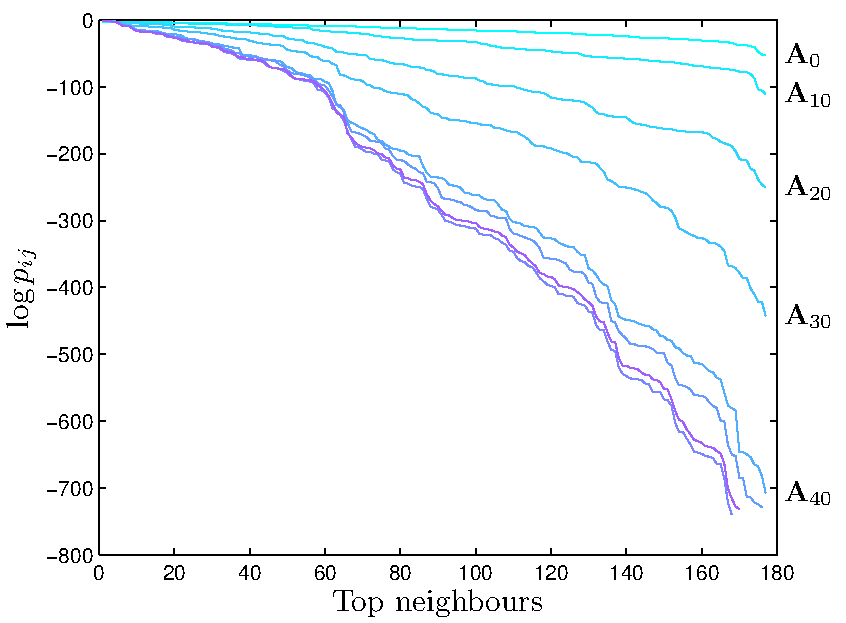
\includegraphics[width=0.7\textwidth]{images/contributions}
	\caption[Evolution of the stochastic assignments $p_{ij}$ during training]{Evolution of the stochastic assignments $p_{ij}$ during training for a given point~$i$. The $y$-axis specifies the contributions $p_{ij}$ on a logarithmic scale. On x-axis we sorted the neighbours in descending order of their contributions. Each curve is associated to a certain linear projection~$\AB_t$, where $t$ denotes the iteration number from the optimization algorithm.}
	\label{fig:contributions}
\end{figure}

The motivation lies in the fact that the contributions $p_{ij}$ decay very
quickly with distance:
 \[
 	p_{ij} \propto \exp\{-d(\AB\xB_i;\AB\xB_j)^2\}.
 \] 
 
The evolution of the contributions during the training period is depicted in
figure \ref{fig:contributions}. We notice that maybe in the first 5-10 iterations the contributions of more than 50 neighbours are significant; after we get out of this regime we can discard a large part of the neighbours and preserve the
accuracy of our estimations. 

\citet{weinberger2007} choose to use only the top $m = 1000$ neighbours for
each point $\xB_i$. Also they disregard those points that are farther away than
$d_{\max}=34$ units from the query point: $p_{ij} = 0, \forall \xB_j$ such that
$d(\AB\xB_i;\AB\xB_j)>d_{\max}$. While useful in practical situations, these
suggestions lack a principled description: how can we optimally choose $m$
and $d_{\max}$ in a general setting? We would also like to be able to estimate
the error introduced by the approximations.

We correct those drawbacks by making use of the KDE formulation of NCA (see
section \ref{sec:cc-kde}) and adapting existing ideas for fast KDE
\citep{deng1995,gray2003} to our particular application. We will use a class of
accelerated methods that are based on data partitioning structures
(e.g., $k$-d trees, ball trees). As we shall see shortly, these provide
us with means to quickly find only the neighbours $\xB_j$ that give significant
values $p_{ij}$ for any query point $\xB_i$. 
%Hence, we will be able to compute an approximated value of the true
%class-conditional probability $p(\xB_i|c) = \sum_{j\in c}
%k(\xB_i|\xB_j),\forall i,c.$
%
%A question still remains: given a point $\xB_i$ how can we \textit{quickly} ?
%It is clear that only the nearby points will contribute to $p_i$, while the
%points that are further away can be ignored. A framework that provides us with
%means of doing this is the $k$-d tree.

\subsection{$k$-d trees}
\label{subsec:k-d-trees}

The $k$ dimensional tree structure ($k$-d tree; \citealp{bentley1975}) organises
the data in a binary tree using axis-aligned splitting planes. The $k$-d tree
places points that live nearby in the 
original geometrical space close in the tree. This makes such structures efficient mechanisms for
nearest neighbour searches \citep{friedman1977} or range searches
\citep{moore1991}.

There are different flavours of $k$-d trees. We choose for our application a
variant of $k$-d tree that uses bounding boxes to describe the position of the
points. Intuitively, we can imagine each node of the tree as a bounding
hyper-rectangle in the $D$ dimensional space of our data. The root node will
represent the whole data set and it can be viewed as a hyper-rectangle that
contains all the data points, see figure \ref{fig:kdtree-1}. In the two-dimensional example presented, the points are enclosed by rectangles. Figures \ref{fig:kdtree-1} to \ref{fig:kdtree-4} show the existing bounding boxes at different levels of the binary tree. To understand how these are obtained, we discuss the $k$-d tree construction.

\begin{figure}
  \centering
  \subfigure[Root
node]{\label{fig:kdtree-1}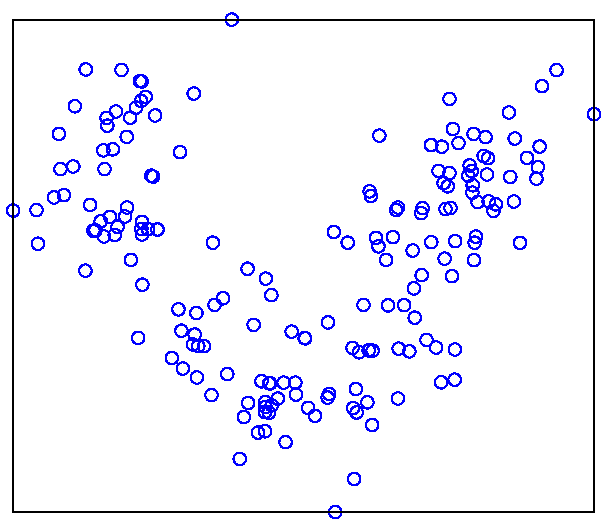
\includegraphics[width=0.45\textwidth]{images/kdtree-1}}
\subfigure[First
level]{\label{fig:kdtree-2}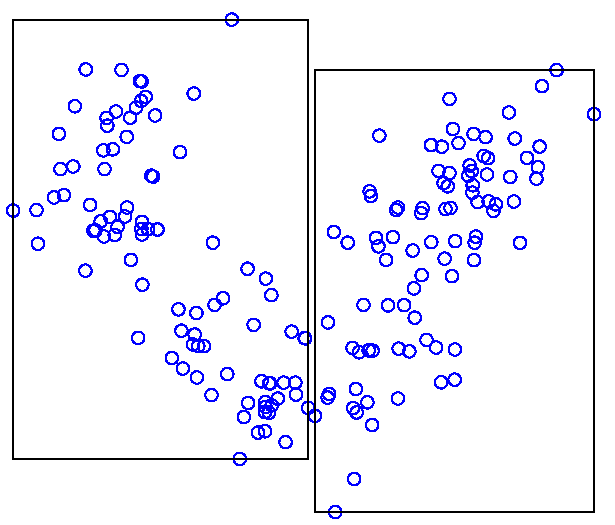
\includegraphics[width=0.45\textwidth]{images/kdtree-2}}
\\
  \subfigure[Second
level]{\label{fig:kdtree-3}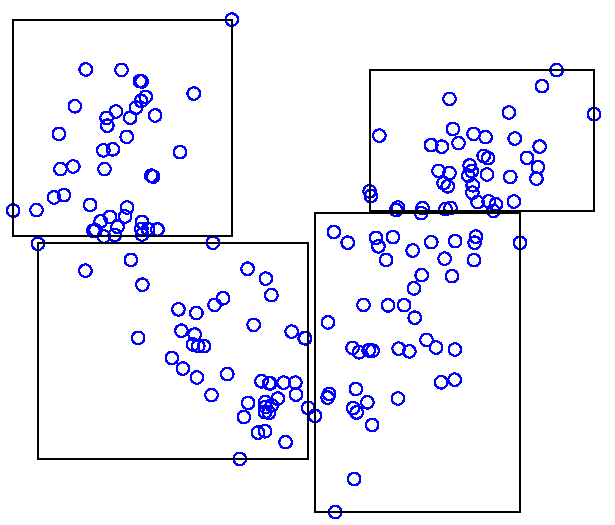
\includegraphics[width=0.45\textwidth]{images/kdtree-3}}
\subfigure[Last
level]{\label{fig:kdtree-4}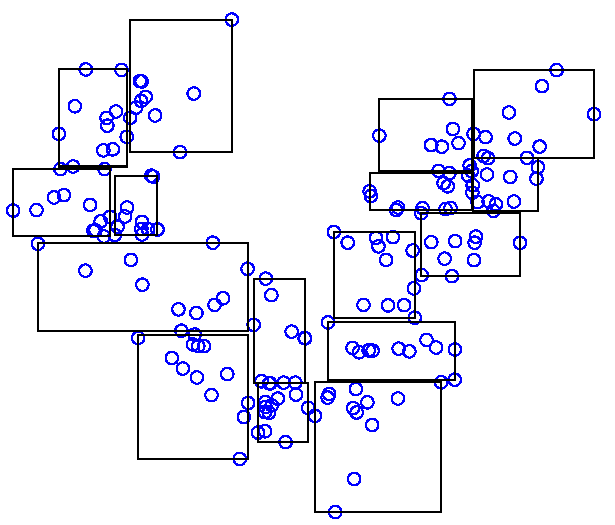
\includegraphics[width=0.45\textwidth]{images/kdtree-4}}
  \caption[$k$-d tree illustration]{Illustration of the $k$-d tree with bounding boxes at different
levels of depths. This figure also outlines the building phases of the tree.}
  \label{fig:kdtree}
\end{figure}

We start building the tree from the root node and then proceed in a recursive manner. At each
node we select which of the points from the current node will be allocated to each of
the two children. Because these are also described by hyper-rectangles, we just have to select a splitting plane. Then the two successors will consist of the points from the two sides of the hyper-plane. 

A splitting hyper-plane can be fully defined by two parameters: a direction $\vec{d}$ on which the plane is perpendicular and a point $P$  that is in the plane. Given that the splits are axis aligned, there are $D$ possible directions $\vec{d}$. We can either choose this randomly or we can use
each of the directions from $1$ to $D$ in a successive manner. A more common approach is to choose $\vec{d}$ to be the dimension that presents the largest
variance: 
\begin{align}
	\vec{d} \leftarrow \operatorname{argmax}_{d} (\max_ix_{id} -
\min_ix_{id}).
	\label{eq:splitting-direction}
\end{align}

Splitting perpendicular on the direction with the greatest variance results in a better clustering of the points and the shape of the bounding boxes will be closer to the shape of a square. Otherwise it might happen that points situated in the same node can still be further away.

Regarding the splitting value $P$, a usual choice is the median value $\tilde{x}_d$ on the previously selected direction $\vec{d}$. This choice of $P$ guarantees a balanced tree which offers several advantages. We can allocate static memory for the entire data structure. This is faster to access than dynamical allocation. Also a balanced tree has a better worst case complexity than an unbalanced one. Other useful implementation tricks that can be applied to balanced $k$-d trees are suggested by \cite{lang2009}.

After the splitting plane is chosen, the left child will contain the points that are on the left of the hyper-plane: 
\begin{align}
\mathcal{D}_{\le \tilde{x}_d} = \{ \xB \in \mathcal{D}_{\xB_i}| x_{d} \le \tilde{x}_d \},
\label{eq:subset-left}
\end{align}
 where $\mathcal{D}_{\xB_i}$ denotes the data points bounded by the current node $\xB_i$. Similarly, the right child will contain the points that are placed on the right of the hyper-plane:
\begin{align}
\mathcal{D}_{> \tilde{x}_d} = \{ \xB \in \mathcal{D}_{\xB_i}| x_{d} > \tilde{x}_d \}.
\label{eq:subset-right}
\end{align}

This process is repeated until the number of points bounded by the current node goes below a threshold $m$. These nodes are the leaves of the tree and they store the data points. The other non-leaf nodes store information regarding the bounding box and the splitting plane. A hyper-rectangle is completely defined by only two $D$-dimensional points, one for the ``top-right'' corner and the other for the ``bottom-left'' corner. 

	\begin{algorithm} 
		\caption{$k$-d tree building algorithm} 
		\label{alg:kd-tree-build}  
		\begin{algorithmic}[1]                    % enter the algorithmic environment
			\REQUIRE Data set $\mathcal{D}=\{\xB_1,\cdots,\xB_N\}$, $i$ position in tree
and $m$ number of points in leaves.
			\IF {$N < m$}
				\STATE Mark node $i$ as leaf: \texttt{splitting\_direction(i)=-1}.
				\STATE Add points to leaf: \texttt{points(i)}$\leftarrow \mathcal{D}$.
				\RETURN
			\ENDIF
				\STATE {Choose direction $\vec{d}$ using equation
\ref{eq:splitting-direction}: \texttt{splitting\_direction(i)=}$d$.}
% 				\STATE {}
				\STATE {Find the median value $\tilde{x}_d$ on the direction $\vec{d}$: \texttt{splitting\_value(i)=}$\tilde{x}_d$.}
				\STATE {Determine the subsets of points that are separated by the resulting splitting plane: $\mathcal{D}_{\le\tilde{\xB}}$ and $\mathcal{D}_{>\tilde{\xB}}$, see equations \ref{eq:subset-left} and \ref{eq:subset-right}.}
				\STATE {Build left child
\texttt{build\_kdtree(}$\mathcal{D}_{\le\tilde{\xB}}$\texttt{,2*i)}.}
				\STATE {Build right child
\texttt{build\_kdtree(}$\mathcal{D}_{>\tilde{\xB}}$\texttt{,2*i+1)}.}
%							$\mathcal{D}_{>\tilde{\xB}}=\{\xB\in\mathcal{D}|\xB>\tilde{\xB}\}$
		\end{algorithmic}
	\end{algorithm}
	
 	The most common operation on a $k$-d tree is the nearest neighbour (NN) search. While we will not apply pure NN for the next method, we will use similar concepts. However, we can do NN retrieval with $k$-d trees after we applied NCA, as suggested by \citet{goldberger2004}. The search in the $k$-d tree is done in a depth-first search manner: start from the root and traverse the whole tree by selecting the closest node to the query point. In the leaf, we find the nearest neighbour from the $m$ points and store it and the corresponding distance $d_\text{min}$. Then we recurse up the tree and look at the farther node. If this is situated at a minimum distance that is smaller than $d_\text{min}$, we have to investigate also that node. Otherwise, we can ignore the node and all the points it contains. Usually, a large fraction of the points can be omitted, especially when the data is clustered.
 	It is important to stress that the performance of $k$-d trees quickly degrades with the dimensionality of the data. 
 	
 	%Hence, it is useful to understand how the search is done and how computational saving are achieved. 
	
%	\begin{itemize}
%		\item 
%		\item So we will be able to efficiently use $k$-d trees only when learning a
%low-rank $\AB$ that projects the data points in a low dimensional space.
%	\end{itemize}
	
%organize the data in a binary tree structure using axis-aligned splitting
%planes of the data space. Each node in the tree represents a data point and it
%also contains a splitting direction (this is usually denoted by an integer from
%1 to $k$). The splitting plane is often chosen to be perpendicular on the
%dimension with the largest variance and to go through the median point (this
%results in a balanced tree). Furthermore, a non-leaf node has two successors:
%the sub-tree rooted at the left successor contains the points that are situated
%at the left of the splitting plane, while the sub-tree rooted at the right
%successor of the splitting plane contains the points that are situated at the
%right of the splitting plane. 

\subsection{Approximate kernel density estimation}
\label{subsec:approx-kde}

The following ideas are mostly inspired by previous work on fast kernel density estimators with $k$-d trees \citep{gray2001, gray2003, gray2003b} and fast Gaussian Processes regression with $k$-d trees \citep{shen2006}.

In kernel density estimation (KDE), we are given a data set~$\mathcal{D}$ and the goal is to compute the probability denisty at a given point using a sum of the contributions from all the points:
\begin{align}
p(\xB_i) = \frac{1}{N}\sum_{j=1}^Nk(\xB_i|\xB_j).
\end{align}

A common class of KDE problems are the $N$-body problems \citep{gray2001} where we have to estimate $p(\xB_i)$ for each data point $\{\xB_i\}_{i=1}^N$ in the data set $\mathcal{D}$. This operation is quadratic in the number of points, as it is the case of NCA\@.

If the number of samples $N$ in $\mathcal{D}$ is sufficiently large, we
expect to accurately approximate $p(\xB_i)$ by using only nearby neighbours of $\xB_i$. 

To illustrate how this works, let us assume we are given a query point $\xB_i$ and a group of points $G$. We try to reduce computations by replacing each individual contribution $k(\xB_i|\xB_j), \xB_j\in G$, with a fixed quantity $k(\xB_i|\xB_g)$. The value of $k(\xB_i|\xB_g)$ is group specific and since it is used for all points in $G$, it is chosen such that it does not introduce a large error. 
A reasonable value for $k(\xB_i|\xB_g)$ is obtained by
approximating each point $\xB_i$ with a fixed $\xB_g$, for example, the mean of the points in $G$. Then we compute the kernel value $k(\xB_i|\xB_g)$ using the estimated $\xB_g$. A second possibility is to directly approximate $k(\xB_i|\xB_g)$. For example:
\begin{align}
  k(\xB_i|\xB_g) = \frac{1}{2}\left( k_{\min} + k_{\max} \right),
  \label{eq:approx-rule}
%\min_jk(\xB_i|\xB_j) + \max_jk(\xB_i|\xB_j)\right).
\end{align} 
where $k_{\min}$ and $k_{\max}$ represent the minimum and maximum contributions for any of the data point in the hyper-rectangle. This last option does not introduce any further computational expense. Both the minimum and the maximum contributions are previously calculated to decide whether to prune or not. Also it does not need storing any additional statistic, such as the mean.

The error introduced by each approximation is bounded by the following quantity:
\begin{align}
\epsilon_{\max} = \frac{1}{2}\left(k_{\max} - k_{\min}\right). 
\end{align}

This can be controlled to be small if we approximate only for those groups that are far away from the query point or when the variation of the kernel value is small within the group.
It is better still to consider the error relative to the total quantity~$p(\xB_i)$. Of course we do not know the total sum we want to estimate in advance, but we can use a lower bound: $p_{\text{SoFar}}(\xB_i) + N_Gk_{\min}$, where $p_{\text{SoFar}}$ denotes the current estimate for $p(\xB_i)$ and $N_G$ is the number of points in the group $G$. Hence, a possible cut-off rule is: 
\begin{align}
  \epsilon_{\max}N_G \le \tau (p_{\text{SoFar}} + N_Gk_{\min}),
\end{align}
where $\tau$ is a constant that controls the error introduced by the approximations: a small $\tau$ means the computations will more accurate, conversely, a large $\tau$ allows more approximations. We use a pruning technique whenever the cut-off rule is true. So in this case it is important the order in which we accumulate. A large $p_{\text{SoFar}}(\xB_i)$ in the early stages will allow more computational savings.

We use $k$-d trees to form groups of points $G$ that will be described as hyper-rectangles. To compute the probability density function $p(\xB_i)$, we start at the root, the largest group, and traverse the tree going through the nearest node each time until we reach the leaf. In this manner, we are able to add large contributions at the beginning. Then we recurse up the tree and visit other nodes only if necessary, when the cut-off condition is not satisfied. We give the exact algorithm for this procedure in the next subsection.

\subsection{Approximate KDE for NCA}
\label{subsec:approx-KDE-for-NCA}
 
We recall that NCA was formulated as a class-conditional kernel density estimation problem, section \ref{sec:cc-kde}. By combining ideas from the previous two subsections, we can develop an NCA specific approximation algorithm.

There are some differences from the classical KDE approximation. In this case, we deal with class-conditional probabilities $p(\AB\xB_i|c),\forall c$. So each class $c$ needs to be treated separately: we build a $k$-d tree with the projected data points $\{\AB\xB_j\}_{j\in c}$ and calculate the estimated probability $\hat{p}(\AB\xB_i|c)$ for each class. Another distinction is that for NCA our final interests are the objective function and its gradient. We can easily obtain an approximated version of the objective function by replacing $p(\AB\xB_i|c)$ with the approximated $\hat{p}(\AB\xB_i|c)$ in equation \eqref{eq:nca-cc-kde-obj}:
\begin{align}
	    \hat{f}(\AB) = \sum_{i=1}^{N} \hat{p}(c_i|\AB\xB_i).
	    \label{eq:nca-cc-kde-obj-approx}
\end{align}

To obtain the gradient of this new objective function we can use equation~\eqref{eq:nca-cc-kde-grad}. The derivative~$\frac{\partial}{\partial \AB}\hat{p}(\AB\xB|c)$ will be different only for those groups where we do approximations. We remind that each individual contribution is given by a normal distribution:
\begin{align}
  k(\AB\xB|\AB\xB_i) \propto \exp\left\{ -(\AB\xB - \AB\xB_i)\tr(\AB\xB - \AB\xB_i) \right\}.
\end{align}

So the gradient of each individual contribution with respect to the linear transformation~$\AB$ will be:
\begin{align}
  \frac{\partial k(\AB\xB|\AB\xB_i)}{\partial \AB} \propto -2\AB k(\AB\xB|\AB\xB_i)(\xB-\xB_i)(\xB-\xB_i)\tr.
\end{align}

We see that using the approximation rule from equation~\eqref{eq:approx-rule} can be applied only for the objective function. We cannot use equation~\eqref{eq:approx-rule} to estimate the gradient, because the gradient depends on the positions of the points in original space and we compute $k_{\min}$ and $k_{\max}$ in the projected space. Both the minimum and the maximum contribution have associated a point in the bounding box. But since the bounding box is formed in the low dimensional space using $\{\AB\xB_i\}_{i=1}^N$ we cannot the points 

%So, for such a group we obtain:
%		\begin{align}
%			\frac{\partial}{\partial \AB} \sum_{j\in G} k(\AB\xB|\AB\xB_j) &\approx
%\frac{\partial}{\partial \AB} \frac{1}{2} \left\{\min_{j\in G}
%k(\AB\xB|\AB\xB_j) + \max_{j\in G} k(\AB\xB|\AB\xB_j)\right\}\notag\\
%			& = \frac{1}{2}\left\{ \frac{\partial}{\partial \AB} k(\AB\xB|\AB\xB_c) %+
%\frac{\partial}{\partial \AB} k(\AB\xB|\AB\xB_f) \right\},
	%	\end{align}
%		where $\AB\xB_c$ denotes the closest point in $G$ to the query point $\AB%\xB$
%and $\AB\xB_f$ is the farthest point in $G$ to $\AB\xB$. Here we made use of the
fact the kernel function is a monotonic function of the distance. This means %that the closest
%point gives the maximum contribution, while the farthest point the
%minimum.
	
	\begin{algorithm}
		\caption{Approximate NCA objective function and gradient computation} 
		\label{alg:cc-kde-nca}  
		\begin{algorithmic}[1]                    % enter the algorithmic environment
			\REQUIRE Projection matrix $\AB$, data set
$\mathcal{D}=\{\xB_1,\cdots,\xB_N\}$ and error~$\epsilon$.
			\FORALL {classes $c$}
				\STATE {Build $k$-d tree for the points in class $c$.}
			\ENDFOR 
			\FORALL {data points $\xB_i$}
				\FORALL {classes $c$}
					\STATE {Compute estimated probability $\hat{p}(\AB\xB_i|c)$ and the
corresponding derivatives $\frac{\partial}{\partial \AB} \hat{p}(\AB\xB_i|c)$ 
using approximated KDE Algorithm:}
%					\STATE {\texttt{[p(c),dp(c)]=NCA\_recursive(kdtree(c))}}
				\ENDFOR
				\STATE Compute soft probability $\hat{p}_i \equiv \hat{p}(c|\AB\xB_i) =
\frac{\hat{p}(\AB\xB_i|c_i)}{\sum_{c}\hat{p}(\AB\xB_i|c)}$.
				\STATE Compute gradient $\frac{\partial}{\partial \AB} \hat{p}_i$ using
equation \eqref{eq:nca-cc-kde-grad}.
				\STATE Update function value and gradient value.
			\ENDFOR
		\end{algorithmic}
	\end{algorithm}
	
	
	
\section{Exact computations}
\label{sec:exact-computations}

	Exact methods are the counterpart of approximate methods. We can have both efficient and exact computations just by modifying the NCA model. Again, the idea is motivated by the rapid decay of the
	exponential function. Instead of operating on very small values, we will make them exactly zero. This is achieved by replacing the squared exponential kernel with a compact support function. So, the points that lie outside the support of the kernel are ignored and just a fraction of the total number of points is used for computing the contributions $p_{ij}$. Further gains in speed are obtained if the search for those points is done with $k$-d trees (the range search algorithm is suitable for this task; \citealp{moore1991}).
	
	The choice of the compact support kernel is restricted by a single requirement: differentiability. We will use the simplest polynomial function that has this property. This is given by the
	following expression:
	\begin{align}
		k_{\text{CS}}(u)=\begin{cases}
			c\;(a^2-u^2)^2& \mbox{if } u \in [-a;+a]\\
			0& \mbox{otherwise},\\
		\end{cases}
		\label{eq:cs-1}
	\end{align}
	where $c$ is a constant that controls the height of the kernel and $a$ is a constant that controls the width of the kernel. In the given context, the kernel will be a function of the distance between two points: $k_{\text{CS}}(u)=k_{\text{CS}}(d_{ij})$, where $d_{ij} = d(\AB\xB_i;\AB\xB_j)$. Note that the constant $a$ can be absorbed by the linear projection $\AB$. This means that the scale of the learnt metric will compensate for the kernel's width. Also the value for $c$ is not important: from equation \eqref{eq:stochastic-neighbours-cs} we see that this reduces. For convenience, we set both $a=1$ and $c=1$. So, we obtain the following simplified version of the kernel:
	\begin{align}
		k_{\text{CS}}(d_{ij})= (1-d_{ij}^2)^2\;\mathrm{I}(\left|d_{ij}\right|\le1),
	\end{align}
	where $\mathrm{I}(\cdot)$ denotes the indicator function: $\mathrm{I}(\cdot)$ return 1 when its argument is
	true and 0 when its argument is false.
	
	Now we reiterate the steps of the NCA algorithm (presented in section \ref{sec:general-presentation}), and replace $\exp(\cdot)$ with $k_\text{CS}(\cdot)$. We obtain the following new stochastic neighbour assignments:
	\begin{align}
		q_{ij} = \frac{k_{\text{CS}}(d_{ij})}{\sum_{k\neq i} k_{\text{CS}}(d_{ik})}.
		\label{eq:stochastic-neighbours-cs}
	\end{align}
	
	These can be compared to the classical soft assignments given by equation \eqref{eq:stochastic-neighbour}. Next we do not need to change the general form of the objective function: 
	\begin{align}
		f_\text{CS}(\AB) = \sum_{i}\sum_{j\in c_i} q_{ij}.
	\end{align}
	
	In order to derive the gradient of the function $f_\text{CS}$, we start by computing the gradient of the kernel:
	\begin{align}
		\frac{\partial}{\partial\AB}k_\text{CS}(d_{ij}) 
		&= 
	\frac{\partial}{\partial\AB}\left[(1-d_{ij}^2)^2\cdot\mathrm{I}(\left|d_{ij}\right|\le
	1)\right]\notag\\
		&= -4\AB(1-d_{ij}^2)  \xB_{ij} \xB_{ij}^\mathrm{T} \cdot
	\mathrm{I}(\left|d_{ij}\right|\le 1),\label{eq:nca-cs-grad-kernel}
	\end{align}
	where $\xB_{ij}=\xB_i-\xB_j$.
	
	The gradient of the new objective function is:
	\begin{align}
		\frac{\partial f_\text{CS}}{\partial \AB}=4\AB\sum_{i=1}^{N}
		\left(
		q_i \sum_{k=1}^N \frac{q_{ik}}{1-d_{ik}^2} \xB_{ik}\xB_{ik}^{\textrm{T}}
		- \sum_{j\in c_i} \frac{q_{ij}}{1-d_{ij}^2}\xB_{ij}\xB_{ij}^{\textrm{T}} 
		\right).
		\label{eq:nca-cs-grad}
	\end{align}
	
	This method can be applied in same way as classic NCA: learn a metric $\AB$ that maximizes the objective function $f_\text{CS}(\AB)$. Since the function is differentiable, any gradient based method is suitable for optimization and can be used on equation \eqref{eq:nca-cs-grad}.
	
	There is one concern with the compact support version of NCA. There are situations when a point $\xB_i$ is placed outside the support of any other point in the data set. Intuitively, this means that the point $\xB_i$ is not selected by any point, hence it is not assigned any class label. Also this causes mathematical problems: as in subsection \ref{subsec:numerical-issues}, the contributions $p_{ij}$ will have an indeterminate value $\frac{0}{0}$. Except of the log-sum-exp trick, the advice from subsection \ref{subsec:numerical-issues} can be applied here as well. A more robust way of dealing with this is discussed in the next section.
	
%	The main concern with this method is what happens when points lie outside the
%	compact support of any other point in the data set. So care must be taken at
%	initialisation. One way would be to initialise with a very small scale $\AB$.
%	However, this means that there is no gain in speed for at least the first
%	iterations. It might be better to use the principal components for
%	initialisation. 
	
\section{NCA with compact support kernels and background distribution}
\label{sec:nca-cs-back}

	\begin{figure}
	  \centering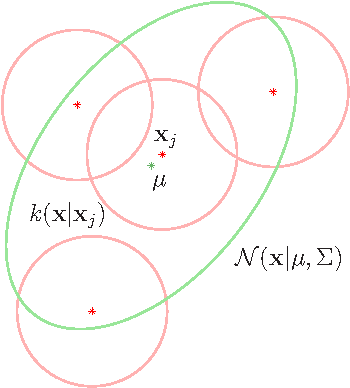
\includegraphics[width=6cm]{images/nca-cs-back}
	  \caption{Neighbourhood component analysis with compact support kernels and
	background distribution. The main assumption is that each class is a mixture of
	compact support distributions $k(\xB|\xB_j)$ plus a normal background
	distribution $\mathcal{N}(\xB|\muB,\SigmaB)$.}
	  \label{fig:cs-back}
	\end{figure}
	
	We extend the previous model to handle cases where points fall outside the support of any other neighbours. The idea is to use  for each class a background distribution that explains the unallocated points. The background distribution should have an infinite support and an obvious example is the normal distribution.
	
	To introduce a background distribution in a principled manner, we return to the class conditional kernel density estimation (CC-KDE) formulation of NCA, section \ref{sec:cc-kde}. First, we recast the compact support NCA in the probabilistic framework and consider each class as mixture of compact support distributions: 
	\begin{align}
		p(\xB_i|c) = \frac{1}{N}\sum_{j\in c} k_\text{CS}(\xB_i|\xB_j),
	\end{align}
	where $k_\text{CS}(\xB_i|\xB_j) = k_\text{CS}(d_{ij})$ and is defined by equation \eqref{eq:cs-1}. Because $k_\text{CS}(\xB_i|\xB_j)$ denotes a distribution, it ought to integrate to 1. For $c=\frac{15}{16}$ and $a=1$ the requirement is satisfied.
	
	We further change the model and incorporate an additional distribution in the class-conditional probability $p(\xB_i|c)$. From a generative perspective this can be interpreted as follows: a point $\xB_i$ is generated by either the compact support distribution from each point $k_\text{CS}(\xB_i|\xB_j)$ or by a class-specific normal distribution $\mathcal{N}(\xB_i|\muB_c,\SigmaB_c)$. So, the distribution $p(\xB_i|c)$ can be written as the sum of these components:
		\begin{align}
			p(\xB_i|c) = \beta \mathcal{N}(\xB_i|\muB_c,\SigmaB_c) + (1-\beta)
	\frac{1}{N_c}\sum_{j\in c} k_\text{CS}(\xB_i|\xB_j),
			\label{eq:nca-cs-back-1}
		\end{align}
	where $\beta$ is the mixing coefficient between the background distribution and
	the compact support model, $\muB_c$ is the sample mean of the class $c$ and $\SigmaB_c$ is the sample
	covariance of the class $c$. The constant $\beta$ can be set to $\frac{1}{N_c+1}$. This will give equal weights to the background distribution and to each compact support distribution. It might be better to treat $\beta$ as a parameter and fit it during training. We expect $\beta$ to adapt to the data set: for example, $\beta$ should increase for data sets with convex classes. 
	
	To finalize this method, we just need to plug equation \eqref{eq:nca-cs-back-1} into
	the set of equations \eqref{eq:nca-cc-kde-bayes}, \eqref{eq:nca-cc-kde-obj} and
	\eqref{eq:nca-cc-kde-grad}. The only difficulty is the gradient computation. We give here only derivatives for each individual component (the full derivations and equations can be found in the Appendix):
	\begin{itemize}
%		\item $\beta = \frac{1}{N_c+1}$ we will give equal weights to the background
%	distribution as to the compact-support distribution. Setting it too large means
%	that the model will favour convex classes. On one hand, this might diminish
%	NCA's power. One of its strengths lies in the ability to work on non-convex
%	classes. On the other hand, some of the classes  This can be fitted as a
%	parameter during the optimization process. The gradient with respect to $\beta$
%	can be easily derived and it is easy to evaluate it as the quantities required
%	for this should also be computed for the function evaluation. 
		\item The gradient of the compact support distribution $k_\text{CS}(\xB_i|\xB_j)$ with respect to $\AB$ is very similar to what is given in equation \eqref{eq:nca-cs-grad-kernel}. The only difference is that in this case we have everything multiplied by the constant $c=\frac{15}{16}$.
		\item For the gradient of the background distribution it is useful to note that projecting the points $\{\xB_i\}_{i=1}^N$
	into a new space $\{\AB\xB_i\}_{i=1}^N$ will change the sample mean $\muB_c$ to
	$\AB\muB_c$ and the sample covariance $\SigmaB_c$ to
	$\AB\SigmaB_c\AB^\mathrm{T}$. Hence, we have:
		\begin{align}
			\frac{\partial}{\partial \AB} \mathcal{N}(\AB\xB_i&|\AB\muB_c, \AB\SigmaB_c
	\AB^\mathrm{T}) = \mathcal{N}(\AB\xB_i|\AB\muB_c, \AB\SigmaB_c
	\AB^\mathrm{T})\notag\\
			&\times \{ -(\AB\SigmaB_c \AB^\mathrm{T})^{-1}\AB\SigmaB_c
			+\vB \vB ^ \mathrm{T} \AB \SigmaB_c - \vB (\xB - \muB_c)^\mathrm{T}
			\},
		\end{align}
		where $\vB = (\AB\SigmaB_c \AB^\mathrm{T})^{-1}\AB(\xB - \muB_c)$.
		\item If we also consider $\beta$ a parameter, we also need the derivative of the objective function with respect to $\beta$. This can be easily obtained, if we use the derivative of the class conditional distribution with respect to $\beta$:
		\begin{align}
			\frac{\partial}{\partial\beta} p(\xB_i|c) 
			=  \mathcal{N}(\xB_i|\muB_c,\SigmaB_c) -
				\frac{1}{N_c}\sum_{j\in c} k_\text{CS}(\xB_i|\xB_j).
		\end{align}
		
	\end{itemize}


\chapter{Evaluation}
\label{ch:evaluation}

This chapter contains the evaluation of the methods proposed in the previous part, chapter~\ref{ch:reducing}. In section~\ref{sec:setup}, we present the data sets and the methodology used for testing. We give details about the parameter choices and set baseline scores obtained by either classical NCA or simple linear projections, such as PCA, LDA or RCA. Results for each individual method are presented in sections~\ref{sec:method-comparison} and~\ref{sec:eval-nca-approx}. A comparison of the methods is shown in subsection~\ref{subsec:eval-comparison} using accuracy versus time plots.

We should mention that we did not include all the results in this chapter to prevent cluttering. Further experimentations can be found in appendix~\ref{app:results}.

\section{Evaluation setup}
\label{sec:setup}

The evaluation was done in terms of two metrics: accuracy and speed. An additional and more subjective criterion is to judge a method by visualizing low dimensional representations of various data sets. We provided 2D plots of the projected data where suitable.

The data sets selected for testing are listed in table~\ref{tab:datasets}. We note that the used data vary both in number of samples~$N$ and in dimensionality~$D$. Even if we concentrate on large amounts of data, we need small data sets to assess the performance of the new models. The methods' speed was tested on the large data sets (\texttt{usps}, \texttt{magic} and \texttt{mnist}). However, the diversity in size and complexity made it difficult to find the optimal selection of parameters. We are aware that there is ``no free lunch'' in accurately solving widely different problems with a fixed model. When concentrating on a single task it is often advised to include prior knowledge into the model. 
% Also it is easier to make minor tweaks of the parameters to boost the performance.

\begin{table}%`
  \centering
    \begin{tabular}{l l c c c} \toprule
	Data set name&Abbrevation&$N$&$D$&$C$\\ 
	\midrule
	Balance scale&\texttt{balance}&$625$&$4$&$3$\\ 
	Ecoli&\texttt{ecoli}&$336$&$7$&$8$\\ 
% 	&\texttt{fruit}&$59$&$3$&$3$\\ 
	Glass identification&\texttt{glass}&$214$&$9$&$6$\\ 
	Ionosphere&\texttt{ionosphere}&$351$&$33$&$2$\\ 
	Iris&\texttt{iris}&$150$&$4$&$3$\\ 
	Landsat satellite&\texttt{landsat}&$6435$&$36$&$6$\\ 
	MAGIC Gamma telescope&\texttt{magic}&$19020$&$10$&$2$\\ 
	MNIST digits&\texttt{mnist}&$70000$&$784$&$10$\\ 
% 	&\texttt{olivetti}&$400$&$4096$&$40$\\ 
	Pima Indians diabetes&\texttt{pima}&$768$&$8$&$2$\\ 
	Image segmentation&\texttt{segment}&$2310$&$18$&$7$\\ 
%	SPECTF heart&\texttt{spectf}&$267$&$44$&$2$\\ 
	Blood transfusion&\texttt{transfusion}&$748$&$4$&$2$\\ 
	USPS digits&\texttt{usps}&$11000$&$256$&$10$\\ 
	Wine&\texttt{wine}&$178$&$13$&$3$\\ 
	Yeast&\texttt{yeast}&$1484$&$8$&$10$\\  
      \bottomrule
    \end{tabular}
    \caption[List of the data sets used for evaluation]{This table presents the characteristics of the data sets used: number of samples $N$, dimensionality of the data $D$ and number of classes $C$. The two digits data sets \texttt{mnist} and \texttt{usps} were downloaded from the following URL \protect\url{http://cs.nyu.edu/~roweis/data.html}. All the others data sets are available in the UCI repository \protect\url{http://archive.ics.uci.edu/ml/datasets.html}.}
    \label{tab:datasets}
\end{table}

For evaluation we used $70\%$ of each data set for training and the remaining $30\%$ was kept for testing. We report standard errors for the mean accuracy averaged over different splits.
We made exceptions for two data sets: \texttt{landsat} and \texttt{mnist}. These are already split into standard training and testing sets. 

The methods we test are: sub-sampling (SS; section~\ref{sec:sub-sampling}), mini-batches (MB; section~\ref{sec:mini-batches}), stochastic learning (SL; section~\ref{sec:stochastic-learning}). For stochastic learning we included two approximated method: the fast kernel density estimation idea (SL-KDE; section~\ref{sec:approximate}) and compact support version of NCA (SL-CS; section~\ref{sec:exact-computations}). Each method has particular parameters that we discuss in its corresponding subsection. 

There are some common choices for all the methods, related to the NCA implementation. For convenience, we review these choices here. We experimented with three optimization methods: gradient ascent with the ``bold driver'' heuristic, conjugate gradients and variants of stochastic gradient ascent with ``early stopping''. For initialization we used the techniques described in subsection~\ref{subsec:initialization}: random initialization, principal component analysis (PCA; \citealp{pearson1901}), linear discriminant analysis (LDA; \citealp{fisher1936}) or relevant component analysis (RCA; \cite{bar2003}). At test time, we did classification using $1$-NN or using an NCA based function as described in subsection~\ref{subsec:doing-classification}. However, we usually present scores using both classification rules.

The experiments were carried in \textsc{Matlab} and most of the implementations are the authors' own work. There are some exceptions however. For conjugate gradients (CG) we used the function \texttt{minimize.m}, written by \citet{rasmussen-online}.\footnote{This is available for download at $<$\url{http://www.gaussianprocess.org/gpml/code/matlab/util/minimize.m}$>$.}
 The RCA implementation was provided by Noam Shental on his web-page.\footnote{The code was downloaded from $<$\url{http://www.openu.ac.il/home/shental/}$>$.}
 Also we used functions from Iain Murray's \textsc{Matlab} toolbox.\footnote{Iain Murray's toolbox is available at $<$\url{http://homepages.inf.ed.ac.uk/imurray2/code/imurray-matlab/}$>$.} Finally, we inspected previous implementations of NCA,\footnote{Implementations of NCA are provided by Laurens van der Maaten in his \textsc{Matlab} Toolbox for Dimensionality Reduction $<$\url{http://homepage.tudelft.nl/19j49/Matlab_Toolbox_for_Dimensionality_Reduction.html}$>$ and by Charless C. Fowlkes on his website $<$\url{http://www.ics.uci.edu/~fowlkes/software/nca/}$>$.}
 even if we did not explicitly make use of them.

\section{Baseline}
\label{sec:baseline} 

We started by implementing the standard NCA algorithm (appendix \ref{app:code-nca-obj}). This is the main baseline against which we compare new models.  
For our first series of experiments, we tried to replicate the work in the original article \citep{goldberger2004}. We encountered some difficulties since no information about their implementation was provided in the paper. Our results are presented in table \ref{table:eval-baseline} (scores are averaged over 40 runs). We randomly initialized the matrix~$\AB$ and optimized it using conjugate gradients (CG) method. This was the easiest thing to do since no parameter tuning is need for CG. We note that the results are similar to those of \citet{goldberger2004}; for the \texttt{ionosphere} data set we obtained slightly worse results.

\begin{table}
  \centering\begin{tabular}{lrcccc}
  \toprule
	  &     & Train score  & \multicolumn{2}{c}{Test scores} & Baseline \\
  \cmidrule(r){3-3} \cmidrule(r){4-5} \cmidrule(r){6-6}
  Data set & $d$ & $f(\AB)$ & $1$-NN & NCA & Eucl. \\
  \midrule
    \texttt{balance}&$2$&$92.86 \pm 0.47$&$90.78 \pm 0.53$&$90.61 \pm 0.55$&\\ 
		    &$D=4$&$95.36 \pm 0.38$&$93.40 \pm 0.47$&$93.04 \pm 0.51$&$76.18$\\ 
    \midrule
    \texttt{ionosphere}&$2$&$98.31 \pm 0.14$&$79.86 \pm 0.75$&$79.74 \pm 0.78$&\\ 
		       &$D=33$&$72.07 \pm 0.71$&$86.22 \pm 0.64$&$72.87 \pm 0.71$&$85.38$\\ 
    \midrule
    \texttt{iris}&$2$&$99.38 \pm 0.11$&$94.94 \pm 0.39$&$94.72 \pm 0.39$&\\ 
		 &$D=4$&$99.48 \pm 0.10$&$95.10 \pm 0.44$&$95.15 \pm 0.44$&$95.53$\\
    \midrule
    \texttt{wine}&$2$&$99.15 \pm 0.14$&$92.4 \pm 1.0$&$92.4 \pm 1.0$&\\ 
		 &$D=13$&$98.95 \pm 0.15$&$95.36 \pm 0.51$&$95.36 \pm 0.51$&$74.53$\\ 
  \bottomrule
  \end{tabular}
  \caption[NCA accuracy on four small data sets]{Accuracy of standard NCA on four small data sets. Scores are averaged over 40 runs. The second column presents the dimensionality~$d$ the data set is reduced to. The last column shows the leave one out cross validation performance on the data set using Euclidean metric.}
  \label{table:eval-baseline}
\end{table}

\begin{table}
  \centering\begin{tabular}{lccc}
  \toprule
  Data set & PCA & LDA & RCA \\
  \cmidrule(r){2-4}
\texttt{usps}&$73.47 \pm 0.13$&$87.44 \pm 0.12$&$87.42 \pm 0.13$\\ 
\texttt{magic}&$77.097 \pm 0.080$&$76.17 \pm 0.29$&$77.574 \pm 0.078$\\ 
\texttt{mnist}&$70.13$&$9.96$&$79.11$\\
\bottomrule
  \end{tabular}
  \caption[Accuracy of PCA, LDA and RCA on large data sets]{Accuracy of three linear transformation techniques applied on the large data sets. We used $1$-NN for classification. Scores are averaged over 20 runs, except for \texttt{mnist} data set. We reduced each data set dimensionality to $d=5$.}
  \label{table:eval-baseline-large-data-sets}
\end{table}
% We used as a baseline a standard NCA implementation . 
% This allowed us to have a baseline to compare the new models against, table \ref{table:eval-baseline}.
% We started testing NCA on small data sets.  This can also be viewed as a replication of the work in the original article \citet{goldberger2004}. The authors did not provide us with any information about their implementation. For our first series of experiments, we used random initialization and we optimized the function using conjugate gradients. The results are averaged over 40 runs. We also considered the score obtained in the original space. We computed this using leave one out cross validation using the Euclidean metric. The results are quite similar to those presented in the original paper.  
% 
% Also for comparison we also offer scores from applying PCA, LDA and RCA followed by $1$-NN.

However, in order to achieve a robust implementation of NCA we had to carry out additional experiments. The lessons learnt were summarized in section~\ref{sec:practical-notes}. We will further see the influence of the implementation tricks in the next part (section~\ref{sec:method-comparison}). Results were shown in section~\ref{sec:practical-notes} and are also attached at the end of the thesis, appendix~\ref{app:results}:
\begin{itemize}
 \item Tables~\ref{table:comp-opts-1} and~\ref{table:comp-opts-2} compare two of the optimization methods: conjugate gradients and gradient ascent with the ``bold driver'' heuristic. We observe that the two methods give close scores on most of data sets. However, the gradient ascent takes longer until it reaches convergence.
 \item Figures~\ref{fig:iris-init}, \ref{fig:balance-init} and~\ref{fig:ecoli-init} illustrate the initialization effect on three data sets: \texttt{iris}, \texttt{balance} and \texttt{ecoli}. RCA seems to be the best option for initialization and we used it in most of our comparisons. However, random projection can also be sometimes surprisingly good as we see in figure~\ref{fig:iris-init-2}. 
\end{itemize}

We could not apply NCA on large data sets (\texttt{usps}, \texttt{magic}, and \texttt{mnist}) since it would have taken far too long. We decided to use as a baseline the linear transformations that we also use for initialization (PCA, LDA and RCA). The results are averaged over different splits of training and testing set and they are listed in table \ref{table:eval-baseline-large-data-sets}. For the \texttt{mnist} data set we have scores of classic NCA \citep{singh2010}. For $d=5$ the accuracy obtained was $91.1\%$ using the $k$NN classifier and $90.9\%$ using the NCA classifier. For the classification procedure \citeauthor{singh2010} learnt the optimal value for $k$ using cross-validation.

\section{Mini-batches methods}
\label{sec:method-comparison}

 The mini-batch methods were compared on the larger data sets: \texttt{usps}, \texttt{magic}, and \texttt{mnist}. We chose to reduce the dimensionality to $d=5$. This decision was partly motivated by the fact that NCA is very effective for reducing the data dimensionality to small values, somewhere around $5$ to $15$. A more principled approach would have been to develop a model choosing algorithm: start with a projection to $d=2$ dimensions and then increase the number of dimensions until the score stops improving. This idea is similar to the ``early stopping'' procedure, and is illustrated for the \texttt{landsat} data set in figure \ref{fig:landsat-evolution}.

  \begin{figure}
   \centering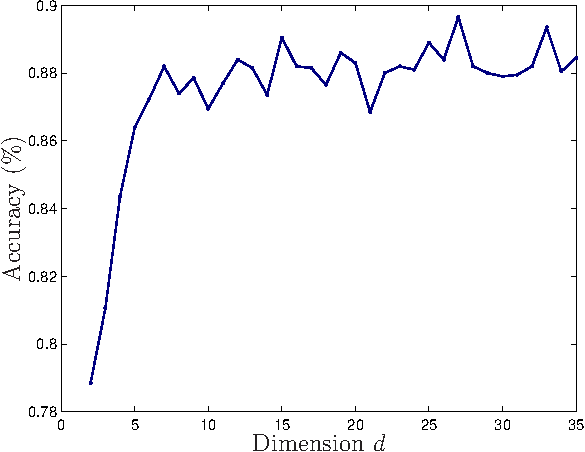
\includegraphics[width=0.6\textwidth]{images/landsat-evolution}
   \caption[Test accuracy as function of reduced dimensionality $d$ on the \texttt{landsat} data]{Evolution of test accuracy as dimensionality increases on \texttt{landsat} data set. We see that NCA operates almost as well in low dimensions ($d=6,\cdots,10$) as in high dimensions ($d>25$). This approach can be used for selecting a suitable dimension to which we project the data.}
   \label{fig:landsat-evolution}
  \end{figure}


  \subsection{Sub-sampling}
  \label{subsec:eval-sub-sampling}

    For sub-sampling we trained NCA on a subset of $n=3000$ samples of the original data. We used conjugate gradients for optimization and RCA linear transformation for initialization. As previously mentioned in section \ref{sec:sub-sampling}, the sub-sampled data has a thinner distribution than the original data which helps the method to obtain good scores at training. But the test performance is hindered because we do not use the true distribution. This is especially evident for the digits data \texttt{usps} and \texttt{mnist} (table \ref{tab:ss}). 
    \begin{table}
    	\centering
    	\begin{tabular}{lccc}
    	\toprule
    	Data set & Train & $1$-NN & NCA \\
    	\cmidrule(r){2-2}\cmidrule(r){3-4}
    	 \texttt{usps}&$99.112 \pm 0.099$&$89.30 \pm 0.18$&$89.41 \pm 0.16$\\
    	 \texttt{magic}&$82.71 \pm 0.41$&$79.25 \pm 0.45$&$80.22 \pm 0.72$\\
    	 \texttt{mnist}&$96.867$&$82.130$&$82.470$\\
    	 \bottomrule
    	\end{tabular}
	\caption[Accuracy for the sub-sampling method on large data sets]{Accuracy scores for the sub-sampling method on the larger data sets. We used RCA for initialization and CGs for optimization. We used a subset of $n=3000$ data points for training and the whole data set for testing.}
	\label{tab:ss}
    \end{table}

    \subsection{Mini-batches}
    \label{subsec:eval-mini-batches}

    We trained NCA using the gradient ascent variant with clustered mini-batches (section~\ref{sec:mini-batches}). For the learning rate, we used an update rule of the form $\frac{\eta}{t+t_0}$. We fixed $\eta=1$ and tuned the other free parameter $t_0$ using cross validation across an exponential scale from $0.1$ to $1000$. After that, a finer tuning was done on a linear scale around the best value of $t_0$. We used $5\%$ of the training set for cross validation to monitor the accuracy score at each iteration. If the performance on the cross validation set does not increase for $25$ iterations, we stop the learning process and return to the previously best parameter.

    To get significant gradients we used large mini-batches $n=2000$. The points in a batch are selected via the recursive projection clustering (RPC; \citealp{chalupka2011}) algorithm. The clustering was done in the low dimensional space, after projecting the points with the current linear transformation matrix~$\AB$.
    The results obtained by the mini-batch method can be found in table \ref{tab:mb}. We note similar scores on \texttt{magic} and better results on the other two data sets.

    \begin{table}
        	\centering
        	\begin{tabular}{lccc}
        	\toprule
        	Data set & Train & $1$-NN & NCA \\
        	\cmidrule(r){2-2}\cmidrule(r){3-4}
        	 \texttt{usps}&$92.00 \pm 0.43$&$91.26 \pm 0.17$&$92.37 \pm 0.17$\\
        	 \texttt{magic}&$80.04 \pm 0.48$&$79.14 \pm 0.52$&$79.8 \pm 1.1$\\
        	 \texttt{mnist}&$87.47 \pm 0.49$&$87.52 \pm 0.36$&$89.88 \pm 0.25$\\
        	 \bottomrule
        	\end{tabular}
		\caption[Accuracy for the mini-batch method on large data sets]{Accuracy scores for mini-batch method on the larger data sets. We used RCA for initialization and the mini-batches were clustered in the low-dimensional space using RPC. The size of a mini-batch was of maximum $n=2000$ data points.}
		\label{tab:mb}
    \end{table}

    \subsection{Stochastic learning}
    \label{subsec:eval-stochastic-learning}

    This method was trained using the variant of stochastic gradient ascent presented in section \ref{sec:stochastic-learning}. We used the same parameters as in the previous section. We considered $n=50$ neighbours to look at for each iteration and computed their contributions with respect to the whole data set. 

    Besides the results on the large data sets (table~\ref{tab:sl-2}), we also present the performance of this method when used for small data sets (table~\ref{tab:sl-1}). We note a considerable improvement on the \texttt{magic} data set compared to the previous two methods. For small data sets, we observe similar results as the baseline NCA. The most important remark is that the classification done using NCA objective function is better than $1$-NN classification. This observation also applies for the large data sets results. More results for this method are in the appendix, table~\ref{app:table:nca-sl-small-1} and~\ref{app:table:nca-sl-small-2}.

    \begin{table}
      \centering\begin{tabular}{lrccc}
      \toprule
	      &     & Train score  & \multicolumn{2}{c}{Test scores}\\
      \cmidrule(r){3-3} \cmidrule(r){4-5}
      Data set & $d$ & $f(A)$ & $1$-NN & NCA \\
      \midrule
	\texttt{balance}&$2$&$88.35 \pm 0.83$&$87.37 \pm 0.49$&$90.45 \pm 0.38$\\  
	&$D=4$&$94.70 \pm 0.87$&$95.32 \pm 0.34$&$96.14 \pm 0.29$\\ 
	\midrule
	\texttt{ionosphere}&$2$&$89.0 \pm 1.7$&$85.71 \pm 0.94$&$87.08 \pm 0.95$\\
	&$D=33$&$92.6 \pm 1.5$&$84.72 \pm 0.57$&$84.34 \pm 0.59$\\ 
	\midrule
	\texttt{iris}&$2$&$96.41 \pm 0.94$&$96.33 \pm 0.57$&$97.00 \pm 0.46$\\ 
	&$D=4$&$97.5 \pm 1.3$&$95.67 \pm 0.71$&$96.11 \pm 0.66$\\ 
	\midrule
	\texttt{wine}&$2$&$98.80 \pm 0.70$&$97.22 \pm 0.65$&$97.50 \pm 0.49$\\ 
	&$D=13$&$99.25 \pm 0.62$&$96.85 \pm 0.41$&$96.85 \pm 0.41$\\ 
      \bottomrule
      \end{tabular}
      \caption[Accuracy for the stochastic learning method on small data sets]{Accuracy scores for stochastic learning method on the small data sets. We used RCA for initialization. The scores are averaged after 20 iterations.}
    \label{tab:sl-1}
    \end{table}

        \begin{table}
            	\centering
            	\begin{tabular}{lccc}
            	\toprule
            	Data set & Train & $1$-NN & NCA \\
            	\cmidrule(r){2-2}\cmidrule(r){3-4}
            	\texttt{usps}&$90.23  \pm 0.50$&$90.68 \pm 0.22$&$92.64 \pm 0.17$\\
            	\texttt{magic}&$78.39 \pm 0.25$&$79.76 \pm 0.13$&$84.49 \pm 0.12$\\
            	\texttt{mnist}&$85.97 \pm 0.37$&$86.07 \pm 0.43$&$89.35 \pm 0.39$\\
            	 \bottomrule
            	\end{tabular}
		\caption[Accuracy for the  stochastic learning method on large data sets]{Accuracy scores for stochastic learning method on the larger data sets. We used RCA for initialization. At each iteration we considered $n=50$ data points.}
		\label{tab:sl-2}
        \end{table}

    \subsection{Comparison}
    \label{subsec:eval-comparison}

    To easily compare the three methods presented, we provide time-accuracy plots (figure \ref{fig:time-accuracy}). We did not record the time taken for smaller data sets, since the classical NCA was usually fast enough. We also included in the plots the method based on the compact support kernels (we discuss its individual scores in subsection \ref{subsec:eval-nca-cs}). 

    In terms of accuracy, all of the NCA variants improve the accuracy over PCA, LDA or RCA\@. Sub-sampling gives comparable results to the other two methods only on the \texttt{magic} data set. This data set has only two classes and a sub-sampled data set does not remove too much information about the decision boundaries. Mini-batches and stochastic learning are similar in accuracy. The proposed methods obtain a slightly worse score than classic NCA on \texttt{mnist}. The performance reported by \citet{singh2010} was around $91\%$, while the mean accuracy for these two methods is about $90\%$. 

    The differences in time varied strongly. We used a logarithmic scale on the time to better discriminate the plotted scores. For each method we show the equidensity contours of the Gaussian distribution. The contours are ellipses, but because of the logarithmic axis they look deformed. 

    The time spent varies even for the same method because the number of iterations until convergence depends on random parameters. We notice a certain trade-off between time and accuracy, especially for the digits data sets.

    We also show low dimensional representations of the data sets for $d=2$ for \texttt{usps} (figure \ref{fig:usps-projection}) and \texttt{magic} (figure \ref{fig:magic-projection}). 
    
      \begin{figure}
		\centering
		\subfigure[\texttt{usps}]{\label{fig:usps}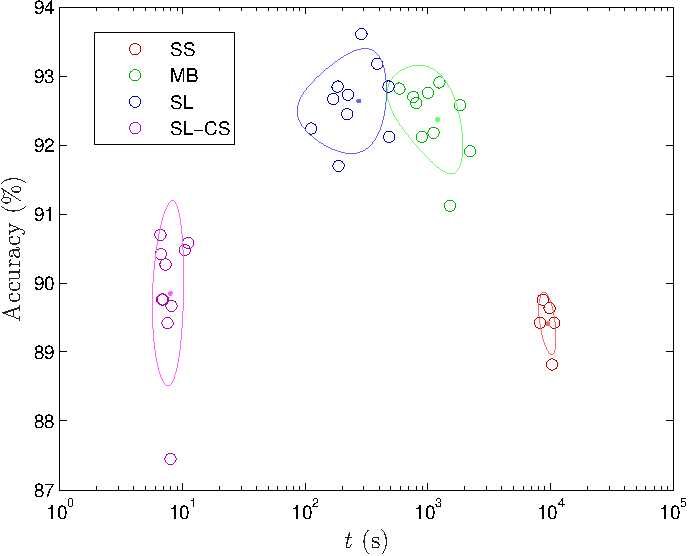
\includegraphics[width=0.55\textwidth]{images/usps-acc-time}}
		\subfigure[\texttt{magic}]{\label{fig:magic}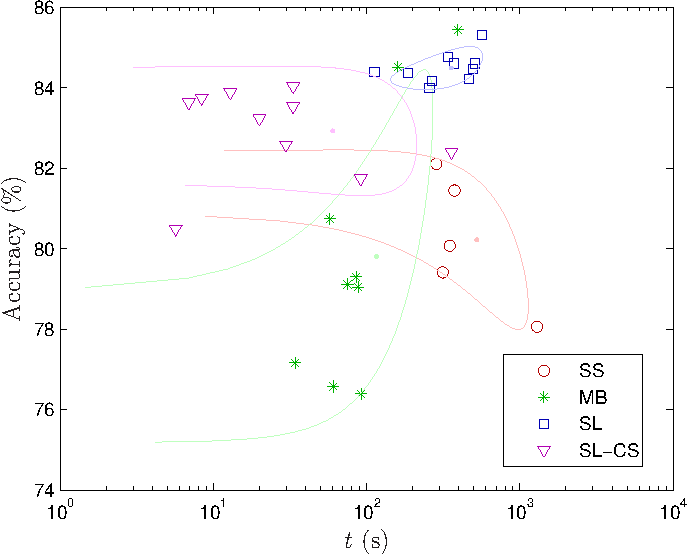
\includegraphics[width=0.55\textwidth]{images/magic-acc-time}}
		\subfigure[\texttt{mnist}]{\label{fig:mnist}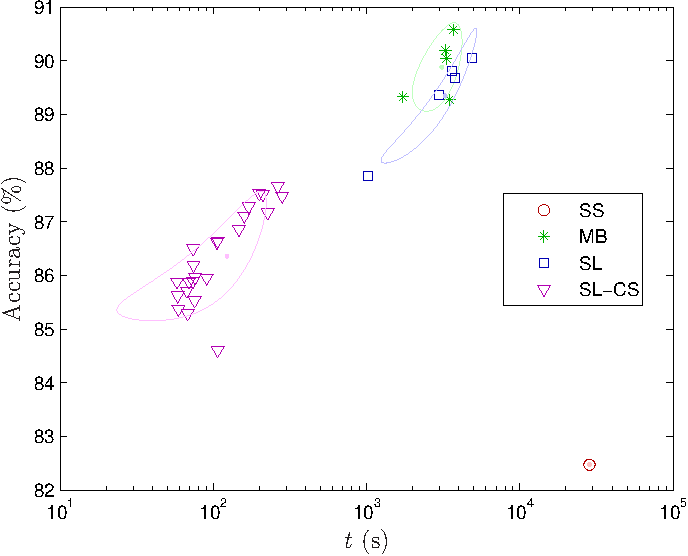
\includegraphics[width=0.55\textwidth]{images/mnist-acc-time}}
		\caption[Time vs. accuracy plots for four of the methods proposed: sub-sampling, mini-batches, stochastic learning and stochastic learning for compact support NCA]{Time vs. accuracy plots on larger data sets for four of the proposed methods: sub-sampling (SS), mini-batches (MB), stochastic learning (SL) and stochastic learning with compact support NCA (SL-CS). For SS we plotted the $1$-NN score, while for the other three the points indicate the NCA score.}
		\label{fig:time-accuracy}
      \end{figure}

     \begin{figure}
		 \centering
			  \subfigure[Mini-batch method]{\label{fig:nca-mb-usps}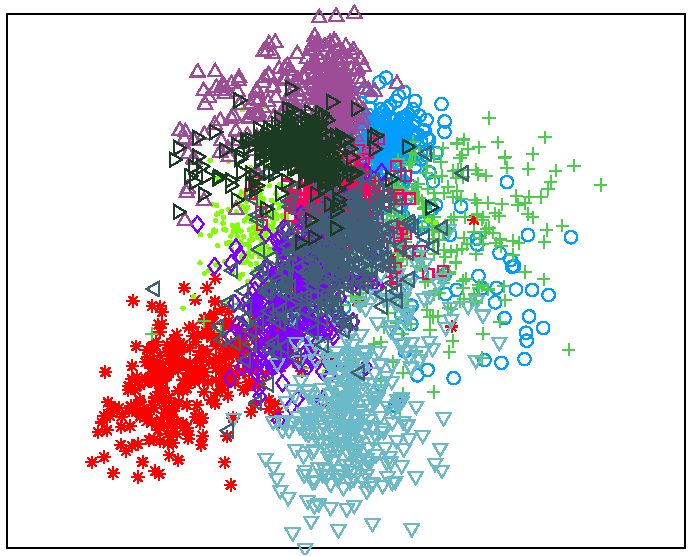
\includegraphics[width=0.45\textwidth]{images/usps-test-mb}}
			    \hspace{0.02\textwidth}
			 \subfigure[Stochastic learning]{\label{fig:nca-sl-usps}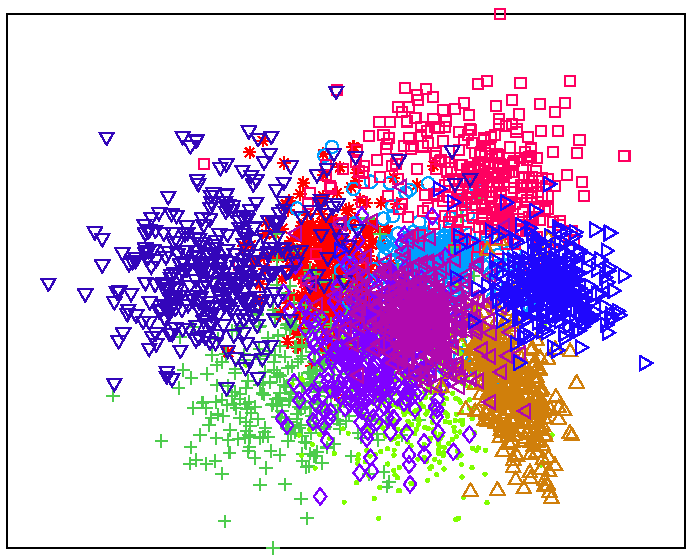
\includegraphics[width=0.45\textwidth]{images/usps-test-snca}}
		\caption[Two dimensional projections of \texttt{usps} data set using two variants of NCA learning: mini-batches and stochastic learning]{Two dimensional projections of \texttt{usps} data set using two variants of NCA learning. The linear transformation was learnt on a training set, and here is plotted the projection of a testing set.}
		\label{fig:usps-projection}
	\end{figure}

     \begin{figure}
		 \centering
			  \subfigure[Mini-batch method]{\label{fig:nca-mb-magic}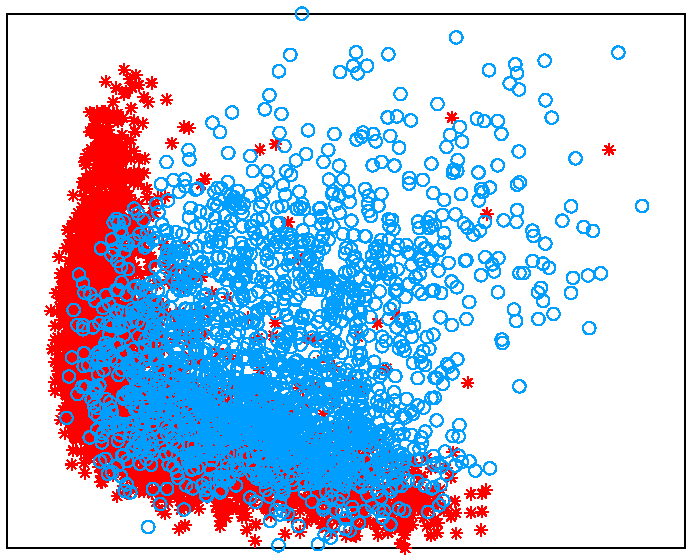
\includegraphics[width=0.45\textwidth]{images/magic-test-mb}}
			    \hspace{0.02\textwidth}
			 \subfigure[Stochastic learning]{\label{fig:nca-sl-magic}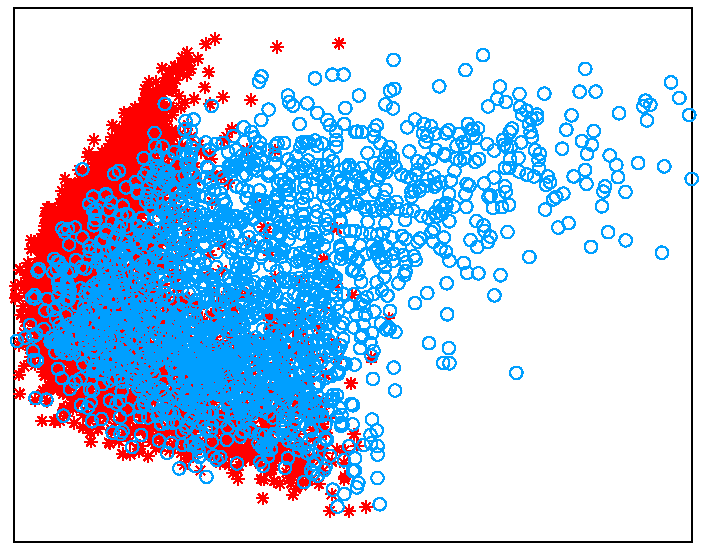
\includegraphics[width=0.45\textwidth]{images/magic-test-snca-cs}}
		\caption[Two dimensional projections of \texttt{magic} data set using two variants of NCA learning: mini-batches and stochastic learning]{Two dimensional projections of \texttt{magic} data set using two variants of NCA learning. The linear transformation was learnt on a training set, and here is plotted the projection of a testing set.}
		\label{fig:magic-projection}
	\end{figure}

\section{Approximate computations}
\label{sec:eval-nca-approx}

The following methods can be applied on classic NCA, but we tested them in conjunction with the stochastic learning procedure to further boost the speed. 

For approximate computations we also tried a more simplistic approach, similar to that of \citet{weinberger2007}: we selected only the first $100$ neighbours for each point and discarded those points whose contribution~$p_{ij}$ is less than $\exp(-30)$. This simple approach gave surprisingly good scores, although we do not present them here.

\subsection{NCA with $k$-d trees}
\label{subsec:eval-nca-k-d-trees}

For the class-conditional kernel density estimation idea we used the algorithm described in section \ref{sec:approximate}. Our $k$-d tree implementation was written in \textsc{Matlab} and, for this reason, it was pretty slow. The code was slower than the simple SL version, because we could not vectorize the recursive computation of the objective function and its gradient. We experimented with kernel density code written in C and mex-ed in \textsc{Matlab} and we think that such an approach can improve the speed. Doing simple kernel density estimation with a C written code proved to be even faster than doing it in \textsc{Matlab}. The short time did not permit us to finalize this approach. We demonstrate that SL with $k$-d trees achieves good results even if we discard a large number of the points. Table \ref{tab:nca-sl-k-d-trees} shows results for this method on the large data sets. We also present how the accuracy and the average number of prunings depend on the maximum error imposed (table \ref{tab:nca-sl-k-d-trees-landsat}). 

\begin{table}
  \centering
 	\begin{tabular}{lcccc}
 	\toprule
 	$\epsilon_{\max}$ & Train & $1$-NN & NCA & Visited points\\
 	\cmidrule(r){2-2}\cmidrule(r){3-4}\cmidrule(r){5-5}
$0$&$87.05 \pm 0.66$&$86.30 \pm 0.32$&$87.87 \pm 0.24$&$80.0 \pm 5.9$\\
$10^{-50}$&$87.50 \pm 0.31$&$86.26 \pm 0.24$&$87.88 \pm 0.20$&$55.1 \pm 5.2$\\
$10^{-20}$&$85.49 \pm 0.89$&$86.32 \pm 0.28$&$87.87 \pm 0.26$&$45.7 \pm 4.1$\\
$10^{-5}$&$87.29 \pm 0.49$&$85.95 \pm 0.19$&$87.63 \pm 0.29$&$22.8 \pm 2.7$\\
$0.01$&$87.34 \pm 0.76$&$86.14 \pm 0.29$&$87.90 \pm 0.24$&$22.1 \pm 4.2$\\
$0.1$&$86.70 \pm 0.39$&$86.12 \pm 0.29$&$88.09 \pm 0.19$&$20.0 \pm 2.0$\\
\bottomrule
  \end{tabular}
  \caption[Accuracy for the  approximated version of NCA trained using stochastic learning on the \texttt{landsat} data set]{Stochastic learning for the approximated version of NCA that uses $k$-d trees. The data set used is \texttt{landsat}. $\epsilon_{\max}$ denotes the maximum error that we accept while approximating the density for a point given a class~$p(\xB|c)$. `Visited points' indicates the fraction of points that are used for computing the function and the gradient.}
  \label{tab:nca-sl-k-d-trees-landsat}
\end{table}


\begin{table}
  \centering
 	\begin{tabular}{lccc}
 	\toprule
 	Data set & Train & $1$-NN & NCA \\
 	\cmidrule(r){2-2}\cmidrule(r){3-4}
 	\texttt{usps}&$89.68 \pm 0.51$&$90.57 \pm 0.20$&$92.67 \pm 0.15$\\
\texttt{magic}&$78.09 \pm 0.37$&$79.68 \pm 0.30$&$84.50 \pm 0.21$\\
\texttt{mnist}&$84.4 \pm 1.4$&$85.5 \pm 1.0$&$88.98 \pm 0.75$\\
  \bottomrule
  \end{tabular}
  \caption[Accuracy for the  approximated version of NCA trained using stochastic learning on large data sets]{Stochastic learning for the approximated version of NCA that uses $k$-d trees. For these experiments we set $\epsilon_{\max}=0.1$.}
  \label{tab:nca-sl-k-d-trees}
\end{table}

\subsection{NCA with compact support kernels}
\label{subsec:eval-nca-cs}

\begin{figure}
	\centering
	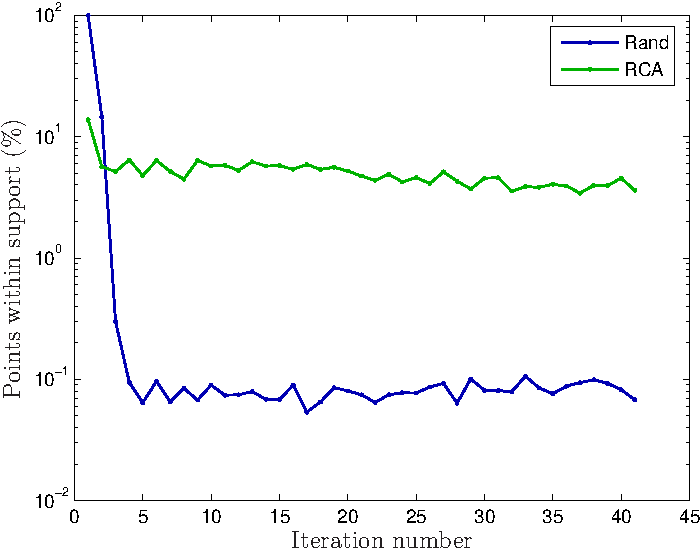
\includegraphics[width=0.6\textwidth]{images/nca-cs-nnzs}
	\caption[Fraction of the points visited during the training of the compact support NCA ]{This figure illustrates how the fraction of the points inspected varies during the learning procedure. When we use random initialization, there are inspected only $0.1\%$ of the points. If RCA is used to initialize the learning algorithm a fraction of about $10\%$ is used.}
	\label{fig:nca-cs-nnzs}
\end{figure}
\begin{figure}
		 \centering
			  \subfigure[Random initialization]{\label{fig:nca-sl-cs-rand}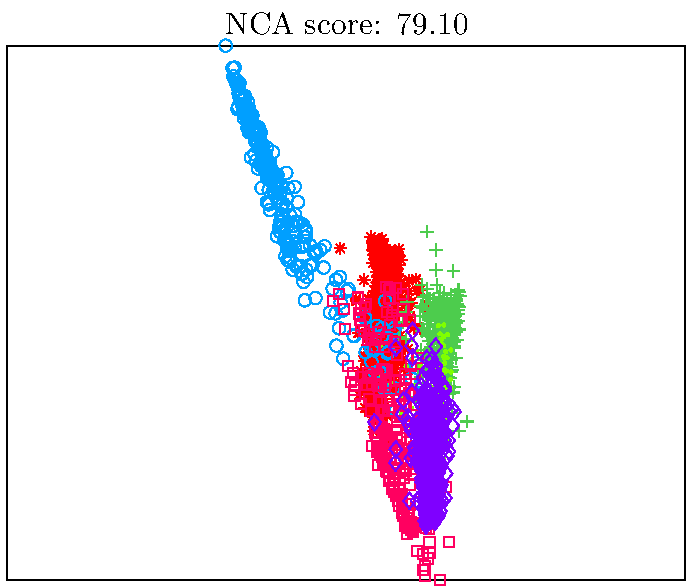
\includegraphics[width=0.45\textwidth]{images/nca-cs-nnzs-rand}}
			    \hspace{0.02\textwidth}
			 \subfigure[RCA initialization]{\label{fig:nca-sl-cs-rca}
\includegraphics[width=0.45\textwidth]{images/nca-cs-nnzs-rca}}
		\caption[Two dimensional projections of the \texttt{landsat} data set using the stochastic learning for the compact support NCA]{Illustration of final two-dimensional projections for the compact support NCA using stochastic learning. There were used two different initialization: random selection of parameters and RCA initialization.}
		\label{fig:landsat-projection}
	\end{figure}

\begin{table}
            	\centering
            	\begin{tabular}{lccc}
            	\toprule
            	Data set & Train & $1$-NN & NCA \\
            	\cmidrule(r){2-2}\cmidrule(r){3-4}
\texttt{usps}&$85.16 \pm 0.33$&$87.02 \pm 0.44$&$89.85 \pm 0.30$\\ 
\texttt{magic}&$76.92 \pm 0.56$&$79.09 \pm 0.42$&$82.92 \pm 0.36$\\ 
\texttt{mnist}&$80.55 \pm 0.28$&$81.96 \pm 0.26$&$86.36 \pm 0.18$\\ 
  \bottomrule
  \end{tabular}
  \caption[Accuracy scores for compact support NCA trained using stochastic learning on large data sets]{Accuracy scores for the compact support NCA method trained using stochastic learning on large data sets.}
  \label{tab:nca-cs-scores}
\end{table}

The compact support version of NCA is easy to implement and it is very fast as we already saw in section \ref{subsec:eval-comparison}. Usually only a small fraction of the points is inspected. In figure \ref{fig:nca-cs-nnzs}, we see how this fraction evolves with the learning process. In the first iterations there might be a larger number of points, but soon this drops off and stabilizes. It might be tempting to start with all the points very close together to ensure that no point is outside the compact support of any other point. This approach has however two drawbacks. Since all the points are in the support of all the other points it means the first iteration will not present any gain in speed. In fact, the first iteration can easily be as expensive as the whole learning process. A second issue is that the gradients will be very large and might ``throw away'' points out of the existing support. An initialization with RCA provided a more stable evolution. We also see that the final projection looks better in the second case (figure \ref{fig:landsat-projection}).

Results that demonstrate performance in terms of accuracy on small data sets are attached in appendix, tables \ref{app:tab:nca-cs-scores-1} and \ref{app:tab:nca-cs-scores-2}. The comparison has as baselines the classical NCA and the extended version of NCA with compact support kernels and background distribution (NCA CS BACK). The results on the large data set are available in table \ref{tab:nca-cs-scores}. 

\section{Recommendations}
\label{sec:eval-recommendations}

When dealing with a large data set, we suggest first trying the stochastic learning for the compact support NCA (NCA CS SL). This method has the advantage of being easy to implement and very fast even for large data sets. However, the speed does come at a cost. We note a slight decrease in accuracy for most experimentations. Nonetheless, applying the NCA CS SL first gives us an idea of how well NCA can perform on a given data set. If one is pleased with the score, it can use the NCA optimized using stochastic learning (NCA SL) or the more sophisticated approximate version that uses $k$-d trees. Usually, these last to methods get an improvement of a couple of percentages in accuracy over NCA CS SL\@. However all the methods offer better scores than the eigendecomposition.

\chapter{Conclusions}
\label{ch:conclusions}

This thesis presented our approach to fast low-rank metric learning. The need for a low rank metric was motivated in the context of $k$NN (chapter~\ref{ch:introduction} and section~\ref{sec:theoretical-background}), but we argue that learning a metric is useful whenever our algorithm relies on dissimilarities. Our efforts were directed towards the already established method, neighbourhood component analysis (NCA; section~\ref{sec:general-presentation}). We introduced a family of algorithms to mitigate NCA's main drawback --- the computational cost. In our attempt of speeding up NCA, we encountered other interesting theoretical and practical challenges. The answers to these issues represent an important part of the thesis (sections~\ref{sec:cc-kde} and~\ref{sec:practical-notes}). We summarize here our main contributions and present the conclusions.
\begin{description}
  \item[Section~\ref{sec:cc-kde}] The class-conditional kernel density estimation (CC-KDE) interpretation offers flexibility to NCA and opens a new range of methods. We can easily change the model in a suitable way by redefining the conditional probability~$p(\xB|c)$. Other advantages are (i) the possibility of including prior class distribution~$p(c)$ into the model and (ii) we can use the posterior probability~$p(c|\xB)$ for classification or in other scenarios that arise in decision theory.
  % for problems with very unbalanced classes and if we want to integrate decision making aspects.
  \item[Section~\ref{sec:practical-notes}] The practical advice in this section is helpful for those who are interested in applying the classic version of NCA\@. The ideas are particularly useful because we are optimizing a non-convex function. We believe that using relevant component analysis (RCA; \citealp{bar2003}) for initialization and conjugate gradients for optimization works best on small and medium-sized data sets. This combination does not require tuning any parameters so it can be readily applied on any data set. Among others, we highlight the dimensionality annealing technique; this look promising: it obtained good projections that seem to avoid local optima.
  \item[Section~\ref{sec:mini-batches}] We gave several ideas of adapting mini-batches (MB) techniques in a suitable way for NCA method. We tested a version based on recursive projection clustering (RPC, \citealp{chalupka2011}). The size of each mini-batch still has to be quite large to get significant gradients (we used $n=2000$). For large data set this already represents a significant improvement in terms of cost, but we question whether there is a more principled method of selecting $n$, the size of a cluster.
  \item[Section~\ref{sec:stochastic-learning}] We presented a stochastic learning (SL) algorithm that is theoretically motivated by stochastic optimization arguments. Empirical investigation demonstrated that this method achieves very close scores to the classic NCA\@. The SL method scales with the number of the points~$N$, but it can be further accelerated using technique presented in sections~\ref{sec:approximate} and~\ref{sec:exact-computations}. A further advantage of SL is that can be used for online learning.
  \item[Section~\ref{sec:approximate}] Using the CC-KDE framework for NCA and inspired from previous work on fast KDE \citep{deng1995, gray2003}, we proposed an algorithm that evaluates efficiently an approximation of the NCA objective function and its corresponding gradient. This method is fastest when combined with SL method. Our experiments suggested that even if we accept a large maximum error~$\epsilon_{\max}=0.1$, we do not seem to lose in accuracy. We noticed a similar behaviour when we did brute pruning.
  \item[Section~\ref{sec:exact-computations}] Further alterations of NCA method are the compact support version (NCA CS) and the compact support and background distribution version (NCA CS BACK). NCA CS achieves considerable speed-ups because we do not have to compute the gradient terms for all the points. Also we observe that it convergences faster than the other methods. However its speed does come at a cost: the accuracy performance is slightly worse than for the rest of the methods. These results might suggest to try a different approach: use a heavy tailed distribution
\end{description}
 
%In chapter~\ref{ch:introduction} we motivated the need for metric learning in the general context of $k$NN, while section~\ref{sec:theoretical-background} advocated for metric learning using more exact mathematical arguments. We showed the equivalence between Mahalanobis metrics and linear transformation which we used for the rest of the thesis. Section~\ref{sec:related-methods} presented some of the related work in Mahalanobis metric learning.

%The focus of this thesis is the NCA method. Chapter~\ref{ch:nca} explores NCA in detail and presents our experience with the method. The theoretical aspect is reviewed in section~\ref{sec:general-presentation} and we also discuss the complexity issues in more detail than they were previously treated. Our main contributions start from section~\ref{sec:cc-kde} which shows a novel interpretation of NCA\@. The class-conditional kernel density estimation, offers certain advantages (like the possibility of integrating class distribution into the model) and opens a new range of methods. In section~\ref{sec:practical-notes} we give practical advice on applying NCA.  Initializing the optimization process with a cheap linear transformation such as LDA or RCA usually results in good final solutions. For the optimization technique there does not seem to be a generally valid answer. Using either regularization or early stopping in conjunction with a NCA-based classification function can boost further the performance. Dimensionality annealing has the premises of an interesting idea, yet we need to further experiment.

%Chapter~\ref{ch:reducing} investigates methods for reducing the computational cost. The classical mini-batches method is modified to work better in a low-rank metric scenario. To do this we used cheap ways of clustering the points in low dimensions and then applied NCA on successive clusters (section~\ref{sec:mini-batches}). We evaluated these methods in an empirical setting (chapter~\ref{ch:evaluation}) and 

\section{Further directions}
\label{sec:further-directions}

This projected involved an abundance of ideas. Unfortunately, in the short time allocated we could only look at a part of the whole picture and we left some paths open. We aim to continue some of the work in the near future. 

We plan to further investigate the automatic differentiation procedure and see whether this is a better idea than symbolic differentiation. Automatic differentiation will help reducing the number of operations needed for the gradient computation, but it might imply a huge memory cost. This trade-off can make automatic differentiation impractical.

The Developing efficient $k$-d tree code for our fast CC-KDE adapted algorithm should prove beneficial. It will allow our methods to run on even larger data sets.

We think that dimensionality annealing approach can be fruitful. However, this idea is still in its infant stages and more experimentation is needed to see whether it can be applied successfully on a variety of data sets. 

Further refinements of our work are still possible. It would be interesting to try a mini-batch and stochastic gradient combined algorithm: cluster points and compute mini-batch mini-batch contributions using a dual tree recursion \citep{gray2003}. 

% Ideas from this thesis can be reused for other distance metric learning methods, with different objective functions (e.g., \citealp{xing2003}). However, this implies losing the convexity.

We believe that other extensions of NCA are possible. For example, a low-dimensional feature extractor could be built using a two step NCA algorithm: first use a diagonal metric~$\SB$ to select the most relevant attributes, followed by 

\appendix
\chapter{MATLAB code}
\lstset{language=Matlab,
   keywords={break,case,catch,continue,else,elseif,end,for,function,global,if,otherwise,persistent,return,switch,try,while},
   basicstyle=\ttfamily,
   keywordstyle=\color{blue},
   commentstyle=\color{dkgreen},
   stringstyle=\color{red},	
   backgroundcolor=\color{white},
   tabsize=2,
   showspaces=false,
   showstringspaces=true}
% All this appendix uses make syntax

\section{NCA objective function}
\label{app:code-nca-obj}
{\singlespace \small
\lstinputlisting{src/nca-obj.m}
}

Notes: 
\begin{enumerate}
  \item \texttt{square\_dist} computes the pairwise distances between two $D$-dimensional sets of points. The function was written by Iain Murray and it can be found in his \textsc{Matlab} Toolbox, available at the following URL: \protect\url{http://homepages.inf.ed.ac.uk/imurray2/code/imurray-matlab/square_dist.m}.
  \item This implementation is suitable for rather small data sets whose pairwise distance matrix can fit in the RAM. If you are dealing with large data sets, it is better to iterate through the data set and compute the distances successively: from a point to the rest of the data set. 
\end{enumerate}

\section{Objective function for stochastic learning}
\label{app:code-snca-obj}
{\singlespace \small
\lstinputlisting{src/snca.m}
}

\chapter{Further results}
\label{app:results}

\section{Initialization}
\label{app:sec:initialization}

This section provides examples of NCA projections on various data sets using different initializations. This is particularly useful to contrast the importance of initializations. Also it shows how NCA typically performs on small sized data sets. 

% The objective function is maximized using conjugate gradients and the entire data sets are used for training. Data sets used are: \texttt{iris}, \texttt{balance} and \texttt{ecoli}. Data set characteristics were presented before in Table, Chapter \ref{ch:evaluation}. 

\begin{figure}
	  \centering
	  \subfigure[NCA projection after random initialization]{\label{fig:iris-init-2}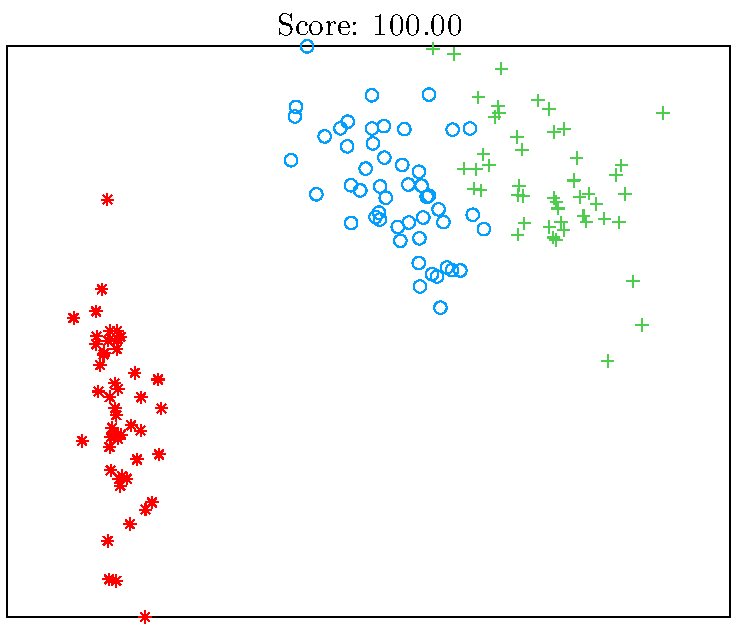
\includegraphics[width=0.47\textwidth]{images/iris-init-2}}
	  \subfigure[NCA projection after PCA initialization]{\label{fig:iris-init-4}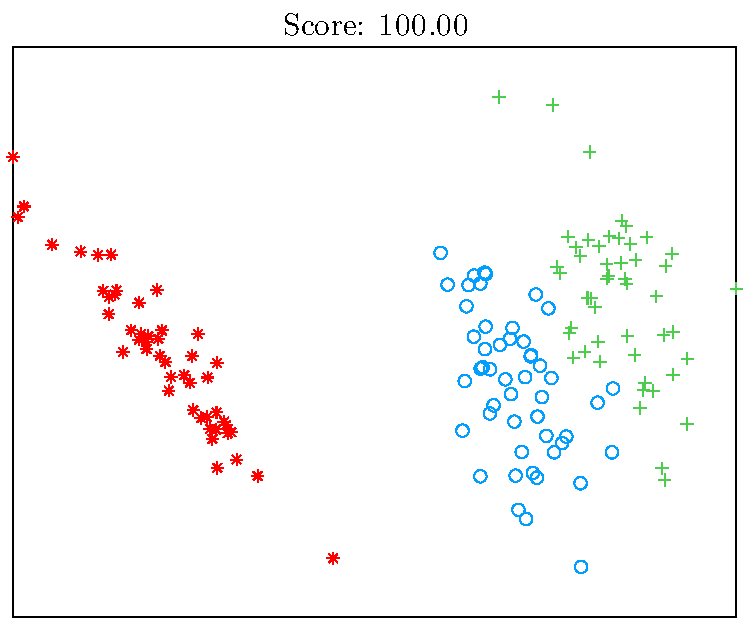
\includegraphics[width=0.47\textwidth]{images/iris-init-4}}
	  \subfigure[NCA projection after LDA initialization]{\label{fig:iris-init-6}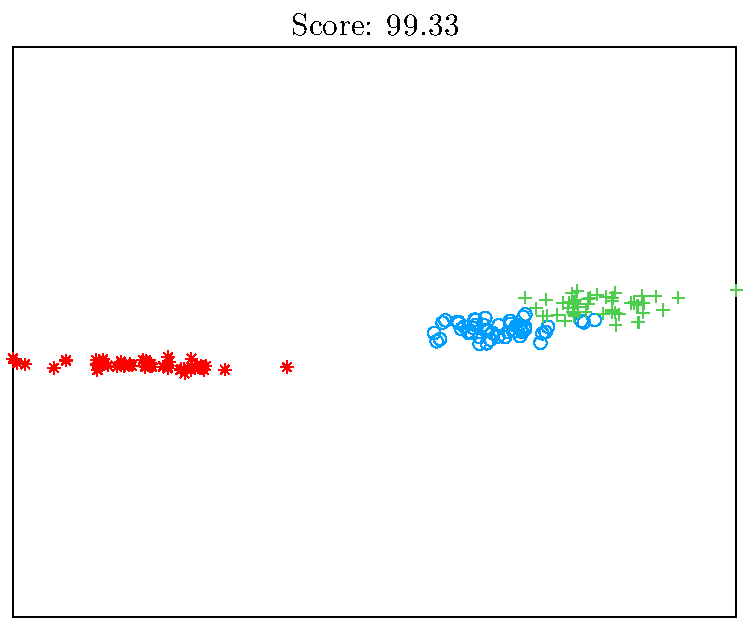
\includegraphics[width=0.47\textwidth]{images/iris-init-6}}
	  \subfigure[NCA projection after RCA initialization]{\label{fig:iris-init-8}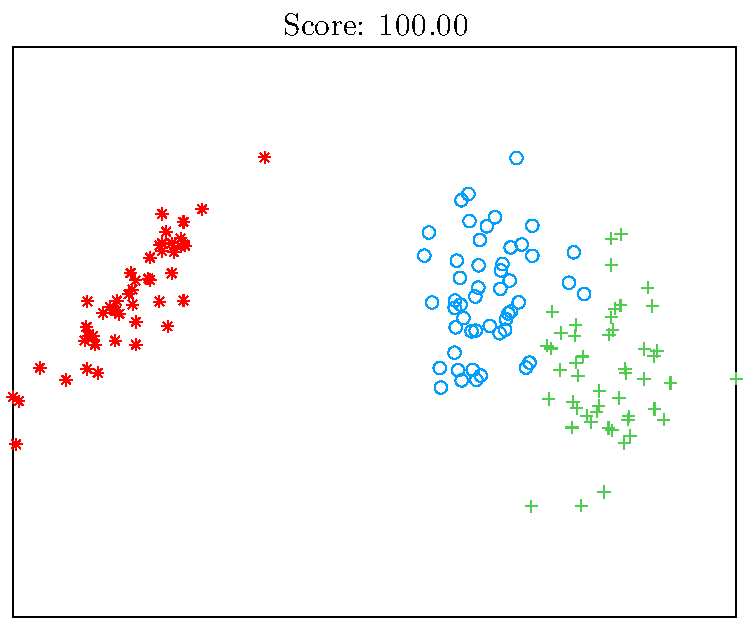
\includegraphics[width=0.47\textwidth]{images/iris-init-8}}
	  \caption{\small Results on \texttt{iris} data set.}
	  \label{fig:iris-init}
\end{figure}

\begin{figure}
	  \centering
	  \subfigure[NCA projection after random initialization]{\label{fig:balance-init-2}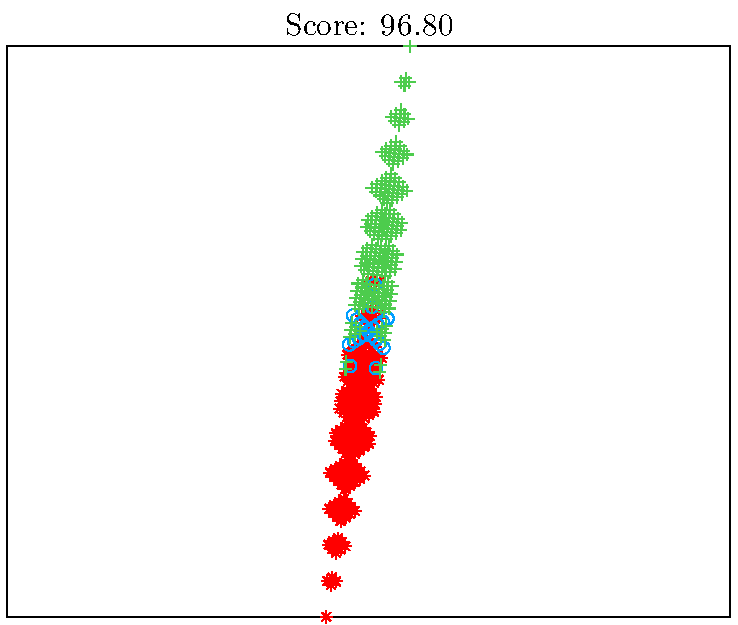
\includegraphics[width=0.47\textwidth]{images/balance-init-2}}
	  \subfigure[NCA projection after PCA initialization]{\label{fig:balance-init-4}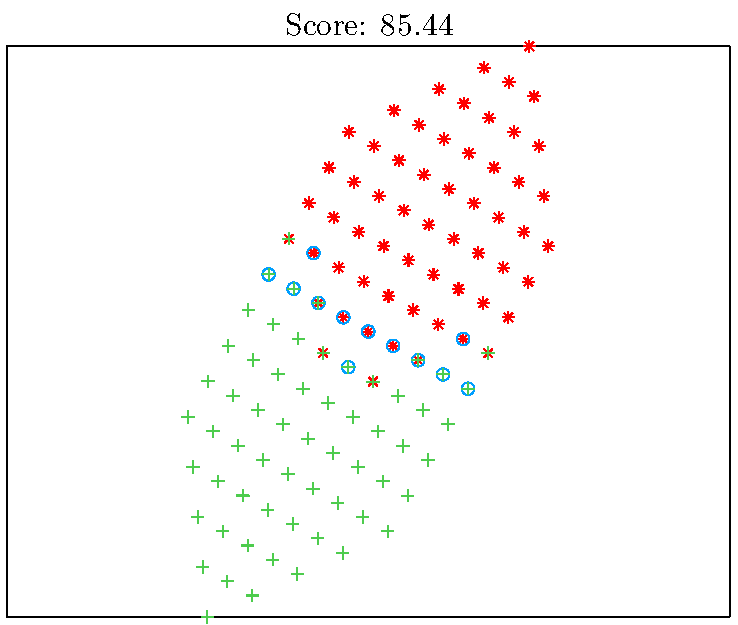
\includegraphics[width=0.47\textwidth]{images/balance-init-4}}
	  \subfigure[NCA projection after LDA initialization]{\label{fig:balance-init-6}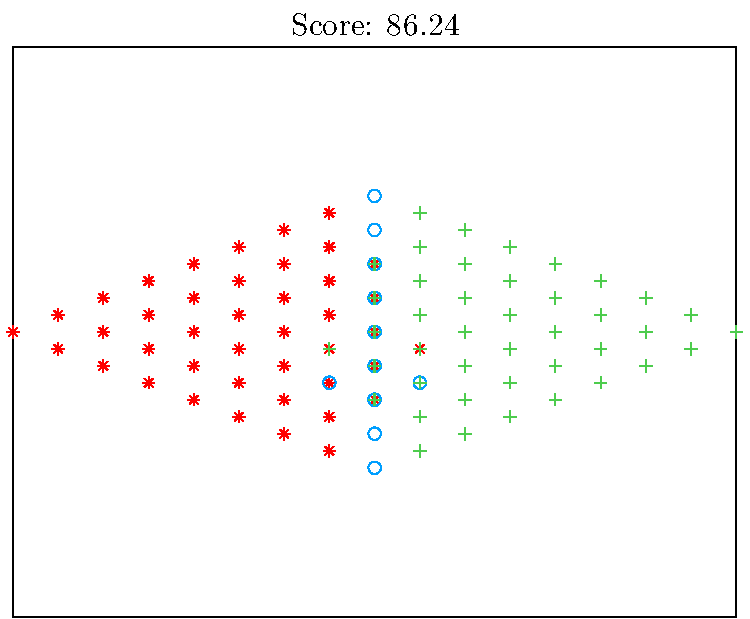
\includegraphics[width=0.47\textwidth]{images/balance-init-6}}
	  \subfigure[NCA projection after RCA initialization]{\label{fig:balance-init-8}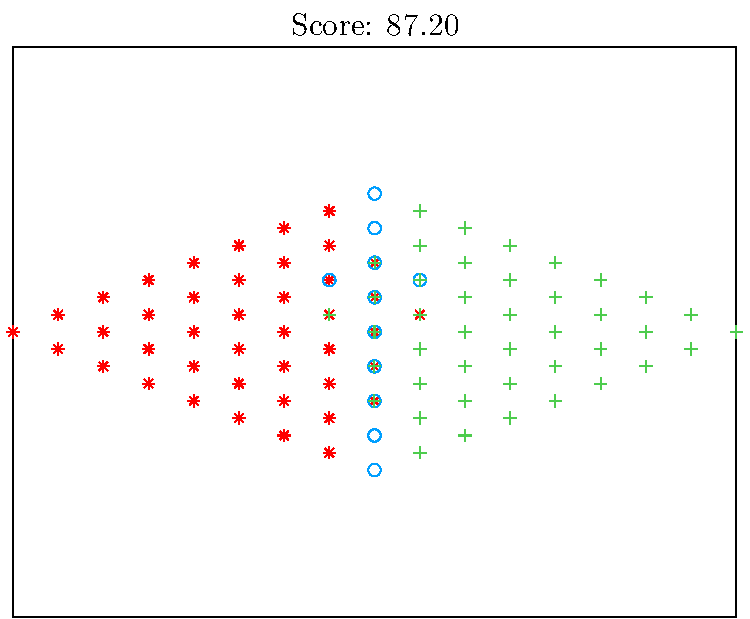
\includegraphics[width=0.47\textwidth]{images/balance-init-8}}
	  \caption{\small Results on \texttt{balance} data set.}
	  \label{fig:balance-init}
\end{figure}

\begin{figure}
	  \centering
	  \subfigure[NCA projection after random initialization]{\label{fig:ecoli-init-2}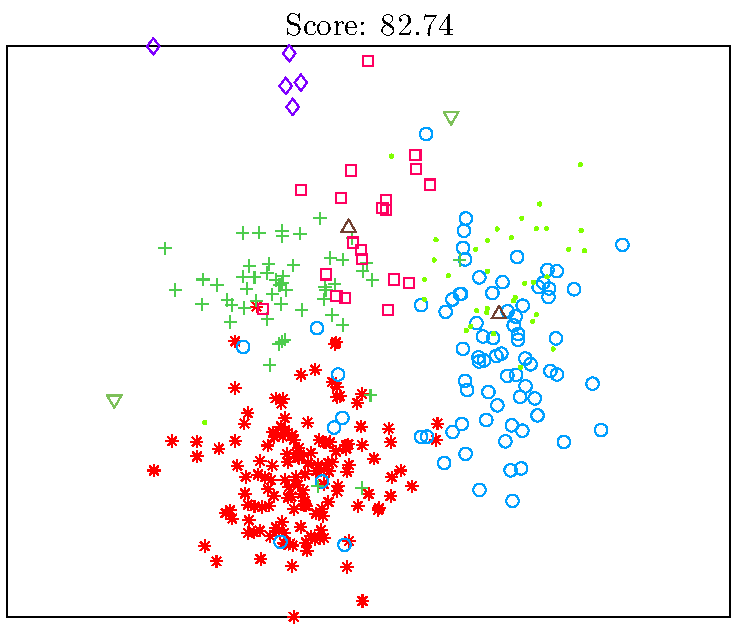
\includegraphics[width=0.47\textwidth]{images/ecoli-init-2}}
	  \subfigure[NCA projection after PCA initialization]{\label{fig:ecoli-init-4}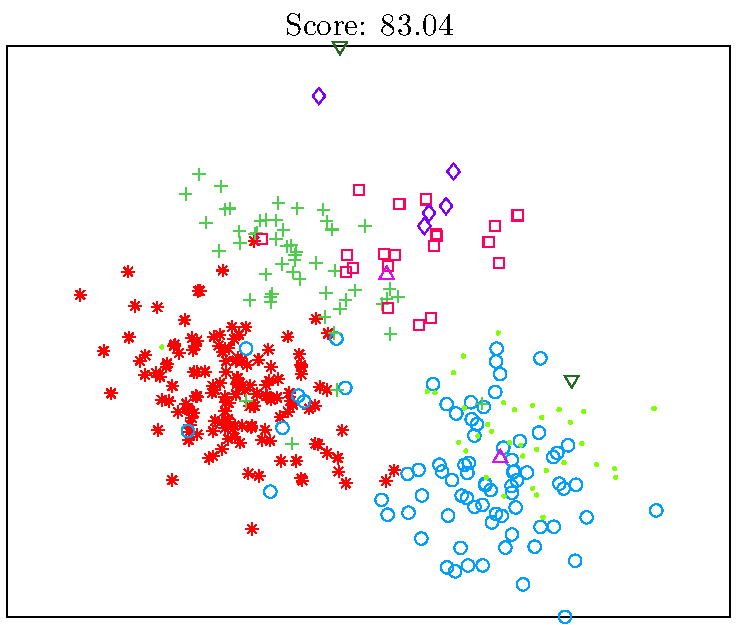
\includegraphics[width=0.47\textwidth]{images/ecoli-init-4}}
	  \subfigure[NCA projection after LDA initialization]{\label{fig:ecoli-init-6}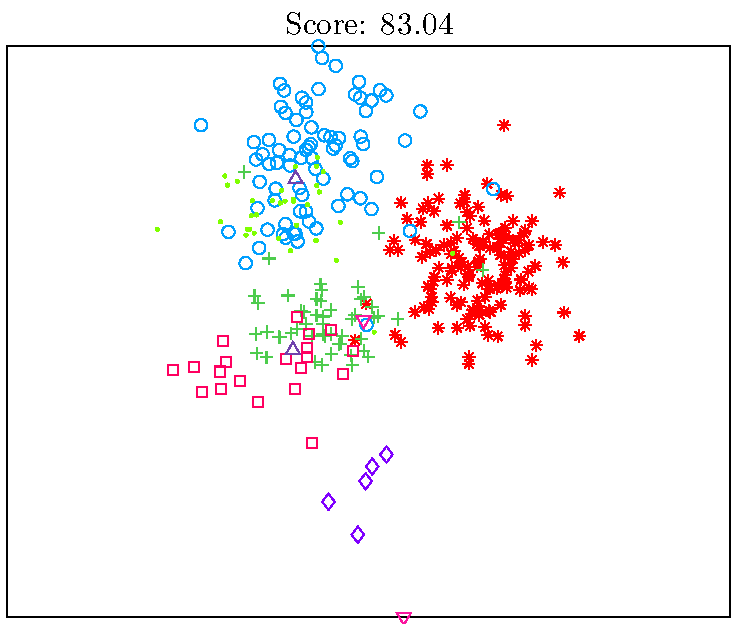
\includegraphics[width=0.47\textwidth]{images/ecoli-init-6}}
	  \subfigure[NCA projection after RCA initialization]{\label{fig:ecoli-init-8}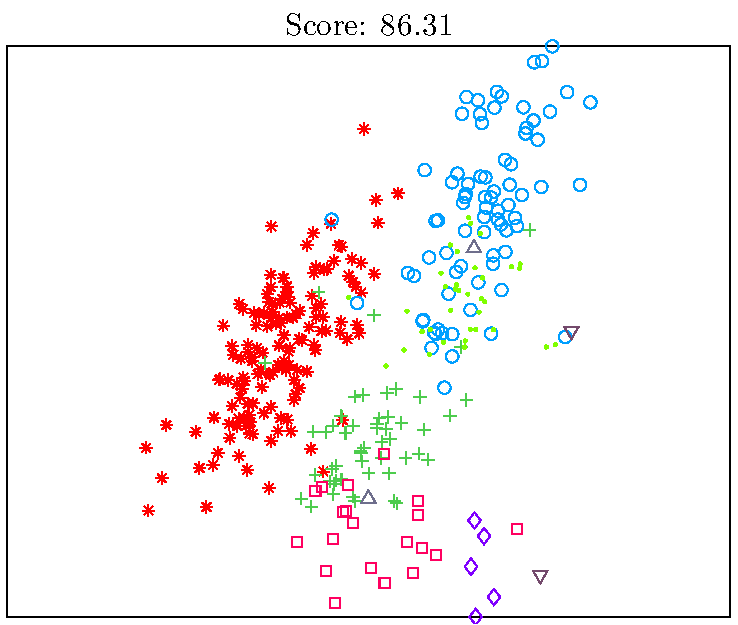
\includegraphics[width=0.47\textwidth]{images/ecoli-init-8}}
	  \caption{\small Results on \texttt{ecoli} data set.}
	  \label{fig:ecoli-init}
\end{figure}

\section{NCA with compact support kernels}
\label{app:sec:nca-cs}

\begin{landscape}
  \begin{table}
    \centering\begin{tabular}{lrcccccc}
      \toprule
      &     & \multicolumn{2}{c}{NCA}  & \multicolumn{2}{c}{NCA CS} & \multicolumn{2}{c}{NCA CS BACK}\\
      \cmidrule(r){3-4} \cmidrule(r){5-6} \cmidrule(r){7-8}
      Data set & $d$ & $1$-NN & NCA & $1$-NN & NCA & $1$-NN & NCA \\
      \midrule
      \texttt{balance}&$2$&$92.74 \pm 0.57$&$92.29 \pm 0.56$&$87.90 \pm 0.68$&$89.04 \pm 0.52$&$89.9 \pm 1.3$&$91.04 \pm 0.94$\\ 
      &$3$&$94.81 \pm 0.52$&$94.87 \pm 0.53$&$89.60 \pm 0.76$&$90.08 \pm 0.60$&$65.2 \pm 3.8$&$87.85 \pm 0.53$\\ 
      &$4$&$95.16 \pm 0.39$&$95.32 \pm 0.33$&$90.82 \pm 0.62$&$92.07 \pm 0.54$&$67.2 \pm 3.4$&$86.91 \pm 0.30$\\ 
      \midrule
      \texttt{glass}&$2$&$53.6 \pm 1.4$&$54.2 \pm 1.5$&$55.8 \pm 1.1$&$57.2 \pm 1.7$&$58.5 \pm 1.2$&$59.4 \pm 1.5$\\ 
      &$3$&$61.8 \pm 1.1$&$60.9 \pm 1.2$&$63.2 \pm 1.4$&$56.3 \pm 1.8$&$61.5 \pm 1.2$&$63.5 \pm 1.1$\\ 
      &$4$&$62.7 \pm 1.4$&$62.2 \pm 1.5$&$62.0 \pm 1.4$&$54.5 \pm 1.6$&$65.2 \pm 1.2$&$65.2 \pm 1.0$\\ 
      &$5$&$64.5 \pm 1.2$&$63.46 \pm 0.97$&$64.9 \pm 1.1$&$57.1 \pm 1.3$&$67.5 \pm 1.2$&$67.2 \pm 1.3$\\ 
      &$9$&$66.5 \pm 1.8$&$65.5 \pm 1.8$&$68.9 \pm 1.5$&$57.8 \pm 1.5$&$68.2 \pm 1.6$&$64.1 \pm 1.3$\\ 
      \midrule
      \texttt{ionosphere}&$2$&$86.23 \pm 0.80$&$86.18 \pm 0.75$&$82.83 \pm 0.74$&$85.33 \pm 0.93$&$85.90 \pm 0.74$&$84.20 \pm 0.74$\\ 
      &$3$&$87.69 \pm 0.62$&$87.64 \pm 0.62$&$85.42 \pm 0.62$&$83.44 \pm 0.69$&$88.11 \pm 0.74$&$84.91 \pm 0.52$\\ 
      &$4$&$87.64 \pm 0.55$&$87.64 \pm 0.57$&$86.08 \pm 0.90$&$83.6 \pm 1.1$&$88.73 \pm 0.92$&$83.7 \pm 1.1$\\ 
      &$5$&$89.39 \pm 0.70$&$89.39 \pm 0.70$&$88.87 \pm 0.61$&$81.46 \pm 0.76$&$86.65 \pm 0.86$&$82.08 \pm 0.98$\\ 
      &$33$&$87.97 \pm 0.68$&$87.97 \pm 0.68$&$86.56 \pm 0.92$&$66.09 \pm 0.95$&$87.26 \pm 0.45$&$84.76 \pm 0.83$\\ 
      \bottomrule
    \end{tabular}
  \caption{luil}
  \end{table}

  \begin{table}
  \centering
    \begin{tabular}{lrcccccc}
    \toprule
	    &     & \multicolumn{2}{c}{NCA}  & \multicolumn{2}{c}{NCA CS} & \multicolumn{2}{c}{NCA CS BACK}\\
    \cmidrule(r){3-4} \cmidrule(r){5-6} \cmidrule(r){7-8}
    Data set & $d$ & $1$-NN & NCA & $1$-NN & NCA & $1$-NN & NCA \\
    \midrule
    \texttt{iris}&$2$&$94.44 \pm 0.51$&$94.11 \pm 0.48$&$95.22 \pm 0.59$&$94.78 \pm 0.72$&$95.22 \pm 0.67$&$95.11 \pm 0.60$\\ 
    &$3$&$95.44 \pm 0.73$&$95.00 \pm 0.75$&$95.33 \pm 0.93$&$95.0 \pm 1.0$&$94.89 \pm 0.80$&$94.2 \pm 1.1$\\ 
    &$4$&$96.56 \pm 0.46$&$96.44 \pm 0.46$&$95.56 \pm 0.54$&$95.67 \pm 0.53$&$95.2 \pm 1.0$&$93.11 \pm 0.95$\\ 
    \midrule
    \texttt{wine}&$2$&$96.67 \pm 0.38$&$96.57 \pm 0.38$&$97.04 \pm 0.51$&$96.94 \pm 0.44$&$97.22 \pm 0.48$&$97.59 \pm 0.46$\\ 
    &$3$&$96.39 \pm 0.48$&$96.39 \pm 0.48$&$96.48 \pm 0.63$&$95.93 \pm 0.65$&$97.22 \pm 0.53$&$97.50 \pm 0.40$\\ 
    &$4$&$96.20 \pm 0.40$&$96.48 \pm 0.41$&$98.06 \pm 0.36$&$98.06 \pm 0.28$&$98.24 \pm 0.33$&$98.89 \pm 0.30$\\ 
    &$5$&$96.57 \pm 0.60$&$96.57 \pm 0.60$&$96.20 \pm 0.71$&$95.00 \pm 0.81$&$97.78 \pm 0.43$&$97.87 \pm 0.40$\\ 
    &$13$&$96.20 \pm 0.48$&$96.20 \pm 0.48$&$95.09 \pm 0.70$&$92.59 \pm 0.92$&$94.63 \pm 0.81$&$98.43 \pm 0.30$\\ 
    \midrule
    \texttt{yeast}&$2$&$42.37 \pm 0.81$&$43.20 \pm 0.84$&$42.57 \pm 0.63$&$48.31 \pm 0.90$&$44.38 \pm 0.66$&$48.24 \pm 0.79$\\ 
    &$3$&$48.06 \pm 0.67$&$48.30 \pm 0.65$&$46.63 \pm 0.72$&$51.6 \pm 1.0$&$47.33 \pm 0.61$&$50.67 \pm 0.55$\\ 
    &$4$&$49.06 \pm 0.47$&$49.14 \pm 0.47$&$49.26 \pm 0.51$&$53.06 \pm 0.94$&$49.93 \pm 0.36$&$53.08 \pm 0.30$\\ 
    &$5$&$50.09 \pm 0.39$&$50.09 \pm 0.38$&$50.16 \pm 0.59$&$52.96 \pm 0.93$&$49.79 \pm 0.62$&$54.54 \pm 0.56$\\ 
    &$8$&$50.66 \pm 0.52$&$50.70 \pm 0.52$&$50.93 \pm 0.44$&$54.89 \pm 0.43$&$48.73 \pm 0.65$&$56.93 \pm 0.62$\\ 
    \bottomrule
    \end{tabular}
  \caption{lals}
  \end{table}

  \begin{table}
    \centering\begin{tabular}{lrcccc}
      \toprule
      &     & \multicolumn{2}{c}{Conjugate gradients}  & \multicolumn{2}{c}{Bold driver}\\
      \cmidrule(r){3-4} \cmidrule(r){5-6}
      Data set & $d$ & $1$-NN & NCA & $1$-NN & NCA \\
      \midrule
	\texttt{balance}&$2$&$92.74 \pm 0.57$&$92.29 \pm 0.56$&$92.05 \pm 0.93$&$92.45 \pm 0.81$\\ 
	&$3$&$94.81 \pm 0.52$&$94.87 \pm 0.53$&$92.79 \pm 0.95$&$92.87 \pm 0.97$\\ 
	&$4$&$95.16 \pm 0.39$&$95.32 \pm 0.33$&$94.18 \pm 0.76$&$94.36 \pm 0.69$\\ 
	\midrule
	\texttt{glass}&$2$&$53.6 \pm 1.4$&$54.2 \pm 1.5$&$58.7 \pm 1.5$&$62.5 \pm 1.4$\\ 
	&$3$&$61.8 \pm 1.1$&$60.9 \pm 1.2$&$66.3 \pm 1.1$&$67.1 \pm 1.1$\\ 
	&$4$&$62.7 \pm 1.4$&$62.2 \pm 1.5$&$65.8 \pm 1.0$&$66.6 \pm 1.3$\\ 
	&$5$&$64.5 \pm 1.2$&$63.46 \pm 0.97$&$66.69 \pm 0.93$&$67.00 \pm 0.87$\\ 
	&$9$&$66.5 \pm 1.8$&$65.5 \pm 1.8$&$66.0 \pm 1.7$&$65.6 \pm 1.7$\\ 
	\midrule
	\texttt{ionosphere}&$2$&$86.23 \pm 0.80$&$86.18 \pm 0.75$&$82.78 \pm 0.98$&$82.78 \pm 0.91$\\ 
	&$3$&$87.69 \pm 0.62$&$87.64 \pm 0.62$&$86.04 \pm 0.83$&$86.08 \pm 0.85$\\ 
	&$4$&$87.64 \pm 0.55$&$87.64 \pm 0.57$&$86.51 \pm 0.73$&$86.51 \pm 0.73$\\ 
	&$5$&$89.39 \pm 0.70$&$89.39 \pm 0.70$&$87.88 \pm 0.64$&$87.88 \pm 0.64$\\ 
	&$33$&$87.97 \pm 0.68$&$87.97 \pm 0.68$&$88.44 \pm 0.59$&$88.44 \pm 0.59$\\ 
      \bottomrule
    \end{tabular}
  \caption{Comparison in terms of accuracy between two possible optimization methods for NCA: conjugate gradients and gradient ascent with the ``bold driver'' heuristic}
  \label{table:comp-opts-1}
  \end{table}

  \begin{table}
  \centering
    \begin{tabular}{lrcccc}
    \toprule
	    &     & \multicolumn{2}{c}{Conjugate gradient}  & \multicolumn{2}{c}{Bold-driver}\\
    \cmidrule(r){3-4} \cmidrule(r){5-6}
    Data set & $d$ & $1$-NN & NCA & $1$-NN & NCA \\
    \midrule
      \texttt{iris}&$2$&$94.44 \pm 0.51$&$94.11 \pm 0.48$&$93.67 \pm 0.82$&$93.78 \pm 0.84$\\ 
      &$3$&$95.44 \pm 0.73$&$95.00 \pm 0.75$&$95.22 \pm 0.72$&$95.33 \pm 0.74$\\ 
      &$4$&$96.56 \pm 0.46$&$96.44 \pm 0.46$&$95.44 \pm 0.76$&$95.56 \pm 0.77$\\ 
      \midrule
      \texttt{wine}&$2$&$96.67 \pm 0.38$&$96.57 \pm 0.38$&$96.30 \pm 0.54$&$96.30 \pm 0.54$\\ 
      &$3$&$96.39 \pm 0.48$&$96.39 \pm 0.48$&$96.57 \pm 0.59$&$96.57 \pm 0.59$\\ 
      &$4$&$96.20 \pm 0.40$&$96.48 \pm 0.41$&$97.13 \pm 0.52$&$97.13 \pm 0.52$\\ 
      &$5$&$96.57 \pm 0.60$&$96.57 \pm 0.60$&$96.76 \pm 0.55$&$96.76 \pm 0.55$\\ 
      &$13$&$96.20 \pm 0.48$&$96.20 \pm 0.48$&$97.22 \pm 0.48$&$97.22 \pm 0.48$\\ 
      \midrule
      \texttt{yeast}&$2$&$42.37 \pm 0.81$&$43.20 \pm 0.84$&$44.65 \pm 0.56$&$46.68 \pm 0.57$\\ 
      &$3$&$48.06 \pm 0.67$&$48.30 \pm 0.65$&$47.06 \pm 0.53$&$47.95 \pm 0.54$\\ 
      &$4$&$49.06 \pm 0.47$&$49.14 \pm 0.47$&$49.48 \pm 0.42$&$49.83 \pm 0.38$\\ 
      &$5$&$50.09 \pm 0.39$&$50.09 \pm 0.38$&$50.16 \pm 0.61$&$50.41 \pm 0.62$\\ 
      &$8$&$50.66 \pm 0.52$&$50.70 \pm 0.52$&$50.19 \pm 0.58$&$50.28 \pm 0.60$\\ 
    \bottomrule
    \end{tabular}
  \caption{Comparison in terms of accuracy between two possible optimization methods for NCA: conjugate gradients and gradient ascent with the ``bold driver'' heuristic}
  \label{table:comp-opts-2}
  \end{table}
\end{landscape}
% \include{appendix/derivations}
%% ... etc ...

%%%%%%%%
%% Any appendices should go here. The appendix files should look just like the
%% chapter files.
%\appendix
%\include{appendix1}
%% ... etc...

%% Choose your favourite bibliography style here.
\bibliographystyle{apalike}

%% If you want the bibliography single-spaced (which is allowed), uncomment
%% the next line.
\singlespace

%% Specify the bibliography file. Default is thesis.bib.
\bibliography{bibliography/thesis}

%% ... that's all, folks!
\end{document}
